\documentclass[a4paper,openany,titlepage]{book}

\usepackage[italian]{babel}
\usepackage[utf8]{inputenc}
\usepackage[T1]{fontenc}
\usepackage{amsmath}
\usepackage{mathtools}
\usepackage{mathematics}
\usepackage{graphicx}



\author{Stefano Garofalo}
\title{Metodi matematici per la fisica}

\begin{document}
\maketitle
\tableofcontents

\toccontents

\chapter{Da dove vengono i numeri complessi}

I numeri complessi vengono dalla ricerca delle soluzione di una equazione cubica da parte di Cardano, cioè le soluzioni di un equazione del tipo:
$$x^3+ax^2+bx+c=0$$
Applicando il cambio di variabile $x=x'-\frac{a}{3}$ otteniamo un equazione sempre di terzo grado, ma nella quale non compare più il termine di secondo grado. A tale equazione applichiamo nuovamente un cambio di variabili $x'=kx''$;ci riconduciamo quindi ad un equazione del tipo:
$$x^3+-3x+a=0$$
A questo punto possiamo scrivere il polinomio come il prodotto di tre binomi di primo grado $(x-x_1) (x-x_2) (x-x_3)$ dove $x_1, x_2$ e $x_3$ sono le tre soluzioni cercate.
Esse devono soddisfare le condizioni:
\begin{itemize}
\item $x_1+x_2+x_3=0$, infatti manca il termine di secondo grado.
\item $-x_1 x_2 x_3=a$, cioè il termine noto.
\end{itemize}
In contemporanea all'uscita della soluzione di Cardano, Ferrari pubblica la sua soluzione per un equazione di quarto grado, procedendo in maniera simile a Cardano: partendo dall'equazione $x^4+ax^3+bx^2+cx+d=0$ ed effettuando la sostituzione $x=x'+\frac{a}{4}$, si ottiene un'altra equazione nella quale non compare il termine di terzo grado.

\section{Il campo complesso}

L'assiomatizzazione del campo complesso, introdotto per la prima volta da Eulero e successivamente rappresentato graficamente come punti sul piano da Gauss, è dovuta ad Hamilton.
Possiamo vedere un numero z complesso come un punto nel piano $\R \times \R$, quindi con coordinate $(x;y)$. Questo tipo di rappresentazione fa sì che i numeri complessi godano di tutte le proprietà della somma, definita come:
$$z+z'=(x;y)+(x';y')=(x+x';y+y')$$
Infatti per questa scrittura valgono le proprietà associativa, commutativa, esiste l'elemento neutro -rappresentato dal vettore nullo $(0;0)$- ed esiste l'elemento opposto -rappresentato da $(-x;-y)$-.
\\
E' facile osservare che la somma di cui si sta trattando in questo caso è una somma vettoriale; infatti, rappresentando i numeri complessi con dei vettori che uniscono l'origine con il punto di coordinate $(x;y)$, si utilizza la regola dei parallelogrammi.
\\
\\
\\
\begin{figure}[h!]
  \centering
    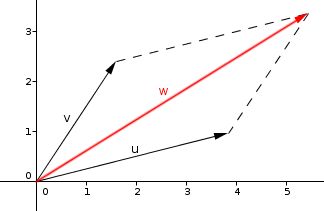
\includegraphics[width=0.5\textwidth]{immagini/sommavettori.png}
\end{figure}

Invece il prodotto fra due numeri complessi viene definito come il prodotto vettoriale, cioè:
$$zz'=(x;y)(x';y')=(xx-yy'';x'y+xy')$$
Anche in questo caso valgono tutte le proprietà del prodotto: commutatività, associatività, esistenza dell'elemento neutro $(1;0)$ e, se $z$ è non nullo, esiste l'inverso $\frac {1}{z}$ .
\\
Oltretutto, vale la proprietà distrubutiva fra il prodotto e l'addizione, cioè:
$$(z_1 +z_2 )z_3 =z_1 z_3 + z_2 z_3$$
La seguente proposizione è stata dimostrata da Hamkel:
\begin{teorema}
$\C$  è il più generale campo che soddisfa tutte le proprietà algebriche, cioè non posso costruire un campo più grande che mantenga verificate tali proprietà.
\end{teorema}
Questo vuol dire che ogni passo avanti corrisponde alla perdita di validità di una proprietà algebrica (ad esempio, nei quaternioni\footnote{Corpo non commutativo che, similmente al campo complesso, ha delle unità ''immaginarie'' (come $i$ per i complessi). Si veda \url{https://it.wikipedia.org/wiki/Quaternione} per approfondimenti (tranquilli, non fa parte del corso).} non vale la commutatività).
\\
Gli elementi del tipo $(x;0)$, cioè gli elementi del campo reale, formano un sottocampo del campo complesso, cioè $\R$ è un sottocampo di $\C$. Questo porta a definire il prodotto per uno scalare:
$$x(x';y')=(x;0) (x';y')=(xx';xy')$$
Sfruttando questa proprietà, vediamo che possiamo scrivere un qualsiasi numero complesso come:
$$(x;y)=x(1;0)+y(0;1)=x+iy$$
Dove $i$ rappresenta l'unità dell'asse immaginario, cioè il vettore (0;1). Si noti che $i$ è anche la radice di -1; infatti:
$$i^2=(0;1) (0;1)=(0-1;0+0)=(-1;0)=-1$$

Definiamo ora il numero complesso coniugato, cioè quel numero (complesso) tale che, se $z$ è scritto come $x+iy$, si ha che il complesso coniugato risulta:
$$\overline{z}=x-iy$$
Risulta ovvio che $\overline{\overline{z}}=z$.

Infine, definiamo il modulo di un numero complesso $z$ come la somma in quadratura della parte reale e della parte immaginaria, cioè:
$$|z|=\sqrt{x^2+y^2}\geq0 \, \, \, \forall z$$
\clearpage
Vediamo ora alcune proprietà dei complessi:
\begin{itemize}
\item $\overline{z_1 z_2}=\overline{z_1} \, \overline{z_2}$
\item $Re(z)=x=\frac{z+\overline{z}}{2}$
\item $Im(z)=y=\frac{z-\overline{z}}{2i}$
\item $|z|=0 \iff z=0$
\item $|z_1 z_2|=|z_1| |z_2|$
\item $|z_1 + z_2| \leq |z_1| + |z_2|$
\end{itemize}
%%Regola del parallelogramma%%
Introduciamo ora due nuovi tipi di rappresentazione del numero complesso $z$. La prima tipologia è detta rappresentazione polare; si ha che:
$$z=x+iy=|z| \left(\frac{x}{|z|}+i \frac{y}{|z|} \right) =|z|(cos(\theta) +i sen(\theta))$$
Infatti sia la parte reale sia la parte immaginaria sono (in modulo) $\leq 1$, e la somma dei loro quadrati dà 1; quindi,  essi rappresentano il seno e il coseno di un angolo $\theta$ tale che $tg(\theta)=\frac{y}{x}$ .
\\
\\
Il secondo tipo di rappresentazione è chiamata rappresentazione esponenziale ed è strettamente legato alla rappresentazione polare; infatti possiamo scrivere:
$$z=|z| (cos(\theta) +i sen(\theta))=|z| e^{i \theta}$$
Questa modalità di rappresentazione dei complessi ci è molto utile nel prodotto fra due numeri complessi; infatti, scrivendo $z_1$ e $z_2$ in forma esponenziale, risulta facile verificare che $z_1 z_2=|z_1||z_2|(cos(\theta + \phi) +i sen(\theta + \phi))$, dove $\theta$ e $\phi$ sono gli angoli relativi ai due numeri complessi presi in considerazione.

Insieme alla rappresentazione esponenziale, introduciamo la funzione argomento principale $Arg(z)$ che associa ad un numero complesso un angolo $\theta \in (-\pi;\pi]$; possiamo quindi scrivere il numero complesso $z$ come:
$$z=|z| e^{i \, Arg(z)}$$

Il motivo per cui $-\pi$ non è incluso nell'intervallo di definizione della funzione argomento principale è legato al fatto che , se così non fosse, avremmo un indecisione sulla scelta del valore dell'angolo da associare; infatti, utilizzando dei semplici limiti, si nota che sul semiasse negativo delle ascisse la funzione $Arg(z)$ presenta una discontinuità di $2i\pi$.
\\
\\
Una formula molto importante per muoversi nel campo complesso è la \textbf{formula di De Moivre}:
$$(cos\theta + i sen\theta)^n =cos(n\theta) + i sen(n\theta)$$
Essa risulta ovvia una volta che si è riscritto il numero complesso in forma esponenziale.\\Vediamo ora come si comporta la funzione esponenziale nel campo complesso; abbiamo che:
$$e^z=e^{x+iy}=e^x e^{iy} =e^x (cos(y)+isen(y))$$
Le proprietà dell'esponenziale nel campo complesso sono:

\begin{itemize}
\item $\overline{e^z}=\overline{e^x e^{iy}}=\overline{e^x} \, \overline{e^{iy}} =e^x e^{-iy} =e^ {\overline{z}}$
\item $e^z =0$ non ha soluzione
\item $e^{z+2i\pi}=e^z$ cioè l'esponenziale è una funzione periodica sull'asse immaginario
\end{itemize}

La funzione esponenziale, infine, è molto utile per riscrivere le funzioni trigonometriche nel campo complesso:

\begin{itemize}
\item $cos(z)=\frac{e^{iz}+e^{-iz}}{2}$
\item $sen(z)=\frac{e^{iz}-e^{-iz}}{2i}$
\item $cosh(z)=\frac{e^z+e^{-z}}{2}$
\item $senh(z)=\frac{e^z-e^{-z}}{2}$
\end{itemize}


%PRECEDENTE: introduzione
\chapter{Funzioni di variabile complessa}

Una funzione $f:D\subset \C \to \C$ è una mappa che manda una variabile $z=x+iy$ in  $w=u+iv$, con $u$ e $v$ che sono funzioni di $x$ e $y$.

Sia ad esempio $f(z)=az$ , con $a \in \C$; essa rappresenta una mappa $z \mapsto w= |a|e^{i\alpha} |z|e^{i \, arg(z)}$; invece una funzione $f(z)=az+b$ opera nella seguente maniera:

\begin{figure}[h!]
    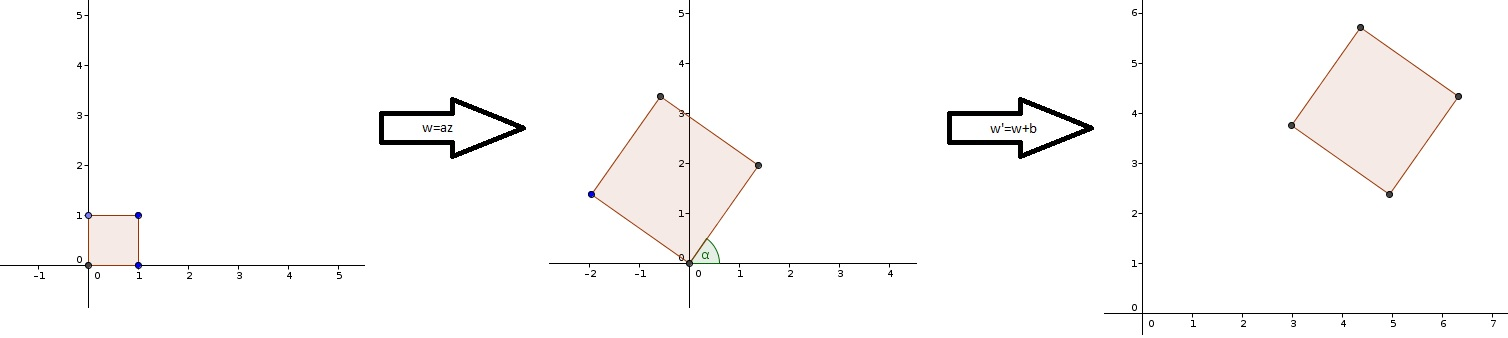
\includegraphics[width=1\textwidth]{immagini/trasformazione.jpg}
\end{figure}
Questo gruppo di trasformazioni è il gruppo delle rototraslazioni nel piano.

Prendiamo ora in considerazione la trasformazione $f(z)=z^2$ e vediamo come opera su una circonferenza:  notiamo che, se prendessimo tutta la circonferenza, otterremmo che la funzione ricopre due volte il piano complesso; per tale motivo, limitiamo il nostro dominio (ad esempio prendendo $Re(z)>0$). Presa la circonferenza di raggio unitario (centrata nell'origine), abbiamo che essa viene mandata nuovamente nella circonferenza di raggio unitario; invece le altre circonferenze centrate nell'origine vengono dilatate $(R>1)$ o ristrette $(R<1)$, mentre, come detto prima, si ha che da un semipiano complesso passiamo all'intero piano complesso.

Questo fatto può essere mostrato anche vedendo il risultato della trasformazione applicata al reticolo coordinato; infatti, abbiamo che:
$$w=z^2=(x+iy)^2=(x^2 -y^2)+2ixy=u+iv$$
A questo punto, ponendo $x$ o $y$ costanti, si ricavano le equazioni del reticolo corrispondente nel piano di arrivo che sarà formato da parabole ad asse orizzontale, con concavità rispetivamente verso sinistra ($x=cost$) e verso destra ($y=cost$).

\begin{figure}[h!]
  \centering
    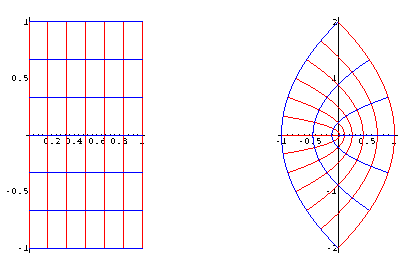
\includegraphics[width=0.4 \textwidth]{immagini/quadrato.png}
\end{figure}

Possiamo ragionare alla stessa maniera anche nel caso opposto, cioè considerando la trasformazione $f(z)=\sqrt{z}$; in questo caso, otteniamo delle iperboli.

\begin{figure}[h!]
  \centering
    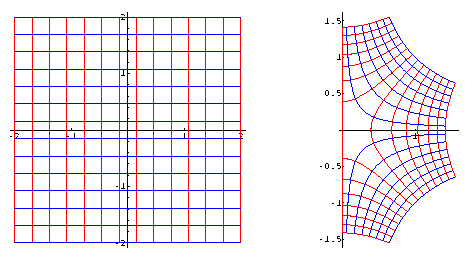
\includegraphics[width=0.4\textwidth]{immagini/quadrattto.png}
\end{figure}

In entrambi i casi, la perpendicolarità fra le linee dei reticoli coordinati viene conservata dalle trasformazioni prese in considerazione, cioè le linee perpendicolari nel piano di partenza lo sono anche nel piano di arrivo.

Infine, vediamo come la trasformazione $f(x)=\frac{1}{z}$ opera sul reticolo coordinato; abbiamo che, se $z=x+iy$, allora:
$$\frac{1}{z}=\frac{1}{x+iy}$$
Quindi, ponendoci sulle linee del reticolo coordinato, otteniamo che per $x$ o $y$ che tendono a $\infty$ la funzione tende a 0, cioè le linee si chiudono in circonferenze centrate su un punto degli assi ($\frac{1}{2x}$ o $ \frac{1}{2iy}$) e  passanti per l'origine.

\begin{figure}[h!]
  \centering
    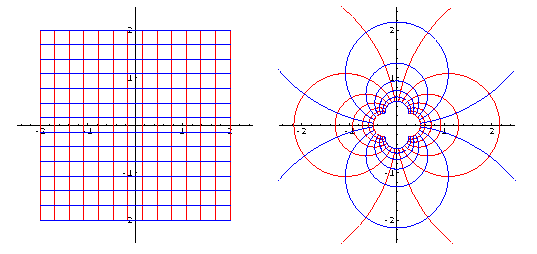
\includegraphics[width=0.4\textwidth]{immagini/inverso.png}
\end{figure}

%SUCCESSIVO: mobius
\chapter{Le trasformazioni di M\"{o}bius}

Le trasformazioni di M\"{o}bius sono marticolari tipi di funzioni della forma:
\begin{equation}
M(z)=\frac{az+b}{cz+d}
\end{equation}
dove $a,b,c,d\in C$ tali che $ad-cb \neq 0$.
\\A tale trasformazione (definita su $\C$ a valori in $\C$) può essere associata una matrice, composta da:
\[
L_M =
\begin{pmatrix}
a	&b\\
c	&d
\end{pmatrix}
\]                                  
La scrittura tramite matrice è comoda nella composizione di due trasformazioni di M\"{o}bius, perchè possiamo trovare la trasformazione associata sempicemente eseguendo il prodotto fra le due matrici; infatti:
$$M'(M(z))=\frac{a'M(z) + b'}{c'M(z) + d'}=\frac{a'(az+b)+b'(cz+d)}{c'(az+b)+d'(cz+d)}=$$
$$=\frac{(a'a+b'c)z+(a'b+b'd)}{(c'a+d'c)z+(c'b+d'd)}$$
Che è lo stesso risultato che otterremmo eseguendo il prodotto fra matrici $L_{M'M}=L_{M'}L_M$.
\\Allo stesso tempo, possiamo facilmente invertire la trasformazione semplicemente trovando la matrice inversa.
 
La mappa lineare $z'=az+b$ e l'inversione $z'=\frac{1}{z}$ sono particolari tipi di trasformazioni di M\"{o}bius con matrice associata:
\[
L_{lineare} =
\begin{pmatrix}
a	&b\\
0	&1
\end{pmatrix}
\]
\[
L_{inversione} =
\begin{pmatrix}
0	&1\\
1	&0
\end{pmatrix}
\]
Possiamo scrivere ogni trasformazione di M\"{o}bius come composizione di mappe lineari e inversioni; infatti, abbiamo che:
\[
\begin{pmatrix}a&b\\c&d\end{pmatrix} = \begin{pmatrix}-\frac{ad-bc}{c}&\frac{a}{c}\\0&1\end{pmatrix}\begin{pmatrix}0&1\\1&0\end{pmatrix}\begin{pmatrix}c&d\\0&1\end{pmatrix}
\]
Dato che sia l'inversione sia la mappa lineare mandano cerchi in cerchi, si ha che ogni mappa di M\"{o}bius conserva tale proprietà.

Per determinare la mappa in questione, basta semplicemente prendere tre punti nel piano di partenza e fissarne le immagini; in questo modo, possiamo fissare univocamente la mappa che unisce i due piani.

Introduciamo ora la Sfera di Riemann, cioè una sfera tangente al piano complesso nell'origine degli assi; dal ''polo nord'', cioè dal punto diametralmente opposto rispetto al punto di  tangenza della sfera, possiamo raggiungere ogni punto del piano attraverso un segmento che intersecherà una e una sola volta la sfera (a parte l'estremo vincolato al polo). In questo modo, abbiamo una corrispondenza biunivoca fra i punti nel piano e i punti sulla sfera.\\
Grazie a questa mappa, possiamo trasferire tutte le operazioni dal piano complesso alla superficie della sfera; ad esempio, la distanza fra due punti viene trasferita sulla sfera come la distanza cordale, cioè:
$$|A'-B'|:=d_{cordale}(A,B) \in [0;2r]$$

\begin{figure}[h!]
  \centering
    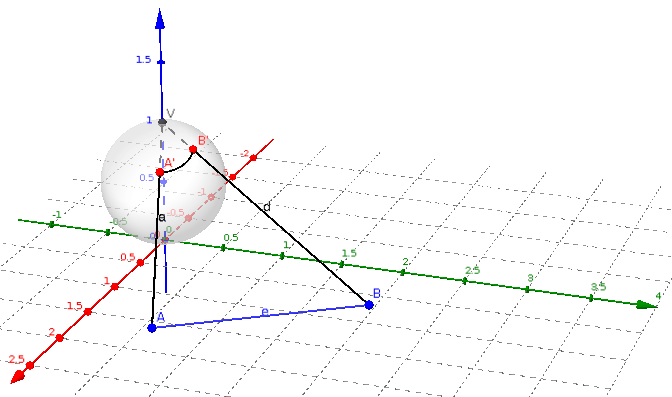
\includegraphics[width=0.5\textwidth]{immagini/sferariemann.png}
\end{figure}

Le trasformazioni di M\"{o}bius che conservano la distanza cordale tra due punti e hanno $ad-bc=1$ corrispondono a matrici $2 \times 2$ in $SU(2)$, cioè lo spazio delle matrici $2 \times 2$ unitarie.
%SUCCESSIVO: \chapter{Completezza di C}

Innanzitutto, definiamo la distanza fra due numeri $z_1$ e $z_2$:
$$d(z_1,z_2)=|z_1-z_2|=\sqrt{(x_1-x_2)^2+(y_1-y_2)^2}$$
Sia ora $\{z_n\}_{n=0}^{\infty}$ una successione in $\C$; come per i reali, il campo $\C$ è completo se, qualora tale successione fosse una successione di Cauchy, allora converge.

Ma procediamo per gradi; iniziamo a definire la convergenza:

\begin{definizione}
 Una successione $z_n$ converge a $z$ se $|z_n-z|\to0$ per $n\to\infty$.
\end{definizione} Ora invece richiamiamo la definizione di successione di Cauchy, vista nel campo reale:
\begin{definizione}
$z_n$ è una successione di Cauchy se $\forall \epsilon$  $\exists N_{\epsilon} : \forall n,m$>$N_{\epsilon} \, |z_n-z_m| < \epsilon$
\end{definizione} Come detto prima, se ogni successione di Cauchy converge allora $\C$ è completo; dimostriamo che si verifica questa situazione:
$$\frac{|x_n-x_m|+|y_n-y_m|}{2}\leq |z_n-z_m|=$$
$$=|(x_n-x_m)+i(y_n-y_m)|\leq |x_n-x_m|+|y_n-y_m|$$
Se $z_n$ è una successione di Cauchy, allora i due addendi dell'ultima disequazione sono entrambi $<\epsilon$ $\forall n,m\leq N_{\epsilon}$; ma allora si ha che $\frac{|x_n-x_m|+|x_n-x_m|}{2} \to 0$ e, dato che è una semisomma di cose positive, $x_n\to x$ e $y_n\to y$, cioè $z_n=x_n+iy_n \to z=x+iy$.

%SUCCESSIVO: variabile-complessa
%PRECEDENTE: completezza-C
\chapter{Le funzioni a variabile complessa}

Sia $f:D\subset \C \to \C$, dove D è un dominio, cioè un insieme aperto e connesso. Ridefiniamo alcune nozioni base:
\begin{definizione}
f si dice continua in $z_0 \in D$ se $\forall \epsilon$>0 $\exists \delta_{\epsilon , z_0} : \, |f(z)-f(z_0)|$<$\epsilon \, \forall z: \, |z-z_0|$<$ \delta_{\epsilon , z_0} $
\end{definizione}
\begin{definizione}
f è derivabile in $z_0$ se esiste finito il
$$\lim_{z \to z_0} {\frac{f(z)-f(z_0)}{z-z_0} =f'(z_0)}$$
La funzione $f(z)$ si dice olomorfa in $z_0$ se esiste $f'(z_0)$, cioè:
 $$\forall \epsilon>0 \, \, \exists \delta_{\epsilon , z_0} : \, \left|\frac{f(z)-f(z_0)}{z-z_0} - f'{z_0}\right|< \epsilon \, \forall z: \, |z-z_0|<\delta_{\epsilon , z_0} $$
\end{definizione}

Introduciamo ora un importante risultato che lega le derivate parziali di una funzione olomorfa, le condizioni di Cauchy-Riemann:
\begin{teorema}(Condizioni di Cauchy-Riemann)\\
Sia f derivabile in $z_0$, dove f e $z_0$ sono rispettivamente della forma $u+iv$ e $x_0+iy_0$. Allora esistono le derivate parziali di $u$ e $v$ -che, in generale, saranno  funzioni di $x$ e $y$- nel punto $(x_0,y_0)$ e valgono:
$$\frac{\partial u}{\partial x}=\frac{\partial v}{\partial y}$$
$$\frac{\partial u}{\partial y}=-\frac{\partial v}{\partial x}$$
\end{teorema}


\begin{proof}
Per ipotesi, esiste il $\lim_{\xi \to 0} \frac{f(z_0+ \xi)-f(z_0)}{\xi} =f'(z_0)$, con $\xi \in \C$. \\Se $\xi=h \in \R$:
$$\frac{u(x_0 +h,y_0)+iv(x_0 +h,y_0)- (u(x_0,y_0)+iv(x_0 ,y_0)) }{h}=$$
$$=\frac{u(x_0 +h,y_0)-u(x_0,y_0)}{h} +i\frac{v(x_0+h,y_0)-v(x_0 ,y_0)}{h} \to f'(z_0) \text{ per } h \to 0$$
Quindi, otteniamo che 
$$\left. f'(z_0)=\frac{\partial u}{\partial x} \right|_{(x_0,y_0)} +i  \left. \frac{\partial v}{\partial x} \right|_{(x_0,y_0)}$$
Se invece $\xi=ih$, abbiamo:
$$\frac{u(x_0,y_0+h)+iv(x_0,y_0+h)-(u(x_0,y_0)+iv(x_0 ,y_0))}{ih}=$$
$$=\frac{u(x_0,y_0+h)-u(x_0,y_0)}{ih}+i\frac{v(x_0,y_0+h)-v(x_0 ,y_0)}{ih} \to f'(z_0) \text{ per } h \to 0$$
Quindi, otteniamo che 
$$f'(z_0)=\left. \frac{1}{i} \frac{\partial u}{\partial y} \right|_{(x_0,y_0)} +\left. \frac{\partial v}{\partial y} \right|_{(x_0,y_0)}=\left. \frac{\partial v}{\partial y} \right|_{(x_0,y_0)}-i \left. \frac{\partial u}{\partial y} \right|_{(x_0,y_0)}$$
Confrontando i due risultati, otteniamo la tesi.

\end{proof}

Se $u$ e $v$ hanno derivate parziali continue in un disco centrato su $z_0$ e valgono le condizioni di Cauchy-Riemann in $z_0$, allora f è derivabile in $z_0$. Inoltre, continuano a valere le regole di derivazione ricavate per funzioni reali a variabile reale.

\subsection{Il significato della derivata}

Nel campo reale, la derivata rappresentava il coefficiente angolare della retta tangente al grafico in un dato punto; che significato ha nel campo complesso?

Consideriamo una curva $\phi :[a,b] \to \C$ passante per $z_0$ e differeziabile con continuità. Supponiamo $\gamma(t_0)=z_0$; $\dot{\gamma}(t_0)$ è il vettore tangente alla curva in $z_0$. Attraverso la funzione $f$ la curva $\gamma$ va a finire in un'altra curva, $f(\gamma(t))$; chi è il vettore tangente a questa nuova curva? Derivando, otteniamo:
$$\left. \frac{d}{dt}f(\gamma(t))\right|_{t_0} =\dot{\gamma}(t_0) f'(\gamma(t_0)) =\dot{\gamma}(t_0) f'(z_0)$$
Quindi la derivata rappresenta un fattore di scala (locale) che modifica la lunghezza del vettore tangente $f'(z_0)$. Vediamo come si comporta la funzione argomento:
$$arg[\dot{\gamma}(t_0) f'(\gamma(t_0))]=arg[\dot{\gamma}(t_0)]+arg[ f'(\gamma(t_0))]$$ cioè, localmente abbiamo una rotazione fissa.

Per capire meglio tale affermazione, immaginiamo di avere due curve incidenti; ognuna di esse avrà un vettore tangente nel punto di intersezione, e tali vettori avranno un angolo fra di essi. Tali vettori, tramite la derivazione, vengono moltiplicati per lo stesso fattore di scala e vengono ruotati dello stesso angolo; quindi l'angolo fra di essi rimane invariato.

Cosa succede se la derivata si annulla? In questi casi, l'angolo fra i vettori tangenti non viene conservato (ad esempio, immagine tramite la funzione $f(z)=z^2$ del quadrato unitario avente vertice nell'origine degli assi).

\section{Altre proprietà}

Abbiamo visto che, se $f(z)=u(x,y)+iv(x,y)$ è una funzione olomorfa, valgono le condizioni di Cauchy-Riemann, cioè $\frac{\partial u}{\partial x}=\frac{\partial  v}{\partial y}$ e $\frac{\partial  u}{\partial y}=-\frac{\partial v}{\partial x}$. Dalle derivate seconde ricaviamo  una proprietà molto utile, cioè che le funzioni $u$ e $v$ sono  armoniche ($\nabla^2 u=0$, $\nabla^2 v=0$); infatti:
$$\frac{\partial^2 u}{\partial x^2}=\frac{\partial^2 v}{\partial y \partial x}=-\frac{\partial^2 u}{\partial y^2} \text{; ma allora si ha che } \frac{\partial^2 u}{\partial x^2}+\frac{\partial^2 u}{\partial y^2}=0 \text{ e, similmente, } \frac{\partial^2 v}{\partial x^2}+\frac{\partial^2 v}{\partial y^2}=0$$
Quindi, attraverso le formule di Cauchy-Riemann, possiamo passare da $u$ a $v$ e viceversa, a meno di una costante (rappresentata dal segno).

%SUCCESSIVO: integrale-complesso
\chapter{L'integrale complesso}

Siamo abituati ad effettuare integrali su linee; abbiamo quindi bisogno di definire una curva in $\C$:

\begin{definizione}

Una curva è una funzione $\gamma:[a;b]\subset\R\to\C$ continua e differenziabile con continuità (cioè esiste il vettore tangente alla curva in ogni punto). La curva ha un verso di percorrenza, che va da $\gamma(a)$ a $\gamma(b)$.

Una curva si dice chiusa se si verifica che $\gamma(a)=\gamma(b)$; se la curva è chiusa e non ha avvolgimenti, cioè se la curva non ha ulteriori intersezioni oltre all'inizio e alla fine della stessa, è detta curva di Jordan.
\end{definizione}
Esempi:
\begin{itemize}
\item Un segmento nel piano complesso, di estremi $z_1$ e $z_2$ è una curva con parametrizzazione $\gamma(t)=z_1+(z_2-z_1)t$, con t$\in$[0;1]. Il vettore tangente è $\dot{\gamma}(t)=z_2-z_1$, cioè è sempre costante in ogni punto della curva.
Un'altra parametrizzazione del segmento è $\tilde{\gamma}(t)=z_1+(z_2-z_1)t^2$, con $t\in[0;1]$; in questo caso, il vettore tangente è $\dot{\tilde{\gamma}}(t)=2t(z_2-z_1)$, cioè non è costante.
\item Una circonferenza di centro $z_0$ e raggio $\rho$ è parametrizzata da $\gamma(\theta)=z_0+\rho e^{i \theta}$, con $\theta \in[0;2\pi]$; il vettore tangente alla curva è $\dot{\gamma}(\theta)=i \rho e^{i \theta}$, cioè è il vettore $\rho e^{i\theta}$ ruotato di $\frac{\pi}{2}$
\end{itemize}
Indicheremo con $\tilde{\gamma}(t)$ o con $-\gamma$ la parametrizzazione che percorre in senso opposto la curva $\gamma$, cioè $\tilde{\gamma}(t)=\gamma(a+b-t):[a;b]\to\C$.
\\
Adesso possiamo introdurre il concetto di integrale nel piano complesso:
\begin{definizione}
Sia $\gamma$ un cammino nel piano complesso con parametrizzazione $\gamma[a;b]\to\C$ differenziabile con continuità; sia f una funzione della variabile z continua sulla curva $\gamma$. Definiamo integrale di una funzione $f$ sulla curva $\gamma$ la quantità:
$$\int_\gamma f(z)dz=\int_a ^b f(\gamma(t))\dot{\gamma}(t)dt=\int_a ^b (u(\gamma_1,\gamma_2)+iv(\gamma_1,\gamma_2))(\dot{\gamma_1}+i\dot{\gamma_2})dt$$ L'integrale di una funzione nel piano complesso è quindi la somma di quattro integrali di Riemann.
\end{definizione}
Introduciamo due importanti disuguaglianze; sia $f:[a;b]\to\C$ continua. Allora:
\begin{itemize}
\item $\left|\int_a^b f(t)dt\right|\leq\int_a^b \left|f(t)\right| dt$. \\ Dimostriamo questo fatto; abbiamo che $\int_a^b f(t)dt$ è un numero complesso, quindi possiamo scriverlo come $\int_a^b f(t)dt=\left|\int_a^b f(t)dt\right|e^{i\theta}$. Possiamo riscrivere l'equazione come $\left|\int_a^b f(t)dt\right|=$ $=e^{-i\theta}\int_a^b f(t)dt=\int_a^b e^{-i\theta} f(t)dt$. Dato che $e^{-i\theta}f(t)$ è un numero reale, posso prenderne la parte reale; ma $Re(z)\leq |z|$, e quindi abbiamo che $\left|\int_a^b f(t)dt\right|=\int_a^b Re(e^{-i\theta} f(t))dt\leq$  $\leq \int_a^b |f(t)|dt$.$_{\Box}$ 
\end{itemize}

\begin{osservazione}
Gli operatori $Re$ e $Im$ possono essere portati dentro e fuori l'integrale liberamente; infatti:
%$$Re\left(\int_a^b f(t)dt\right)=Re\left(\int_a^b(u+iv)dt\right)=Re\left(\int_a^bu \, dt\right)+Re\left(\int_a^b iv \, dt\right)=\int_a^bu \, dt=\int_a^b Re(f(t))dt$$%
$$Re \int_a^b f(t)dt=Re \int_a^b(u+iv)d=Re \int_a^bu \, dt +Re \int_a^b iv \, dt =\int_a^bu \, dt=\int_a^b Re(f(t))dt$$
\end{osservazione}

\begin{itemize}
\item \textbf{Disuguaglianza di Darboux}: $\left|\int_{\gamma} f(z) dz\right| \leq L[\gamma] \, \sup_{z \in \gamma} |f(z)|$, dove $L[\gamma]$ rappresenta la lunghezza della curva $\gamma$. Dimostriamo questa disuguaglianza: 
$$\left|\int_{\gamma} f(t) dt\right|=\left|\int_a ^b f(\gamma(t))\dot{\gamma}(t)dt\right| \leq \int_a ^b |f(\gamma(t))| \, |\dot{\gamma}(t)|dt \leq$$
$$\leq \sup_{t \in [0;1]} |f(\gamma(t))|\, \int_a ^b \sqrt{\dot{\gamma_1 ^2}+\dot{\gamma_2 ^2}}dt=\sup_{t \in [0;1]} |f(\gamma(t))| \, L[\gamma] \leq L[\gamma] \sup_{z \in \gamma} |f(z)|$$
\end{itemize}
Un'altra proprietà utile da tenere a mente è la seguente:
$$\int_{-\gamma} f(z) dz=-\int_{\gamma} f(z) dz$$

\section{La funzione primitiva}

Introduciamo ora il concetto di primitiva per una funzione complessa:
\begin{definizione}
Sia $f:D \subset \C \to \C$ una funzione continua su D. La funzione F si dice primitiva di f in D se F è olomorfa su D e vale che $F'(z)=f(z)$ $\forall z \in D$.
\end{definizione}
Se F è primitiva di f, abbiamo che:
$$\int_{\gamma}f(z)dz=\int_a ^b f(\gamma(t))\dot{\gamma}(t)dt=\int_a ^b F'(\gamma(t))\dot{\gamma}(t)dt=\int_a ^b \frac{d}{dt}(F(\gamma(t)))dt=F(\gamma(b))-F(\gamma(a))$$ Oltretutto, abbiamo che, se $\gamma$ è chiusa, allora l'integrale risulta nullo.

Sia $f(z)=z^n$; la sua primitiva è $F(z)=\frac{z^{n+1}}{n+1}$ per $n \neq -1$. Poniamo $D\equiv \C \backslash \{(0;0)\}$. Prendiamo poi la circonferenza centrata nell'origine di raggio 1, parametrizzata da $\gamma(\theta)=e^{i \theta}$; l'integrale della funzione $z^n$ sulla curva $\gamma$ è:
$$\int_{\gamma} z^n dz=\int_0 ^{2\pi} e^{i n \theta} i e^{i \theta} d\theta=i \int_0 ^{2\pi} e^{i (n+1) \theta} d\theta=$$
$$=i \int_0 ^{2\pi} \left[cos((n+1)\theta)+isen((n+1)\theta)\right] d\theta= \left\{
  \begin{array}{l l}
    0 & \quad \text{se $n \neq -1$}\\
    2 \pi i & \quad \text{se $n=-1$}
  \end{array} \right.$$

La funzione $\frac{1}{z}$ è olomorfa in $\C \backslash \{(0;0)\}$, La sua primitiva è $Log(z)$, olomorfa in $\C \backslash \{(x;0) : x \in (0;+\infty]\}$. Se come cammino prendiamo la circonferenza precedentemente utilizzata, il valore dell'integrale non è nullo, perchè il cammino scelto attraversa la zona in cui la curva non è olomorfa. Prendiamo la curva $\gamma_{\epsilon}$, cioè l'arco di circonferenza che unisce i punti $-1-i\epsilon$ e $-1+i\epsilon$ senza attraversare il semiasse negativo delle ascisse, e calcoliamo l'integrale della funzione $\frac{1}{z}$ su di essa:
$$\int_{\gamma_{\epsilon}}=Log(-1+i\epsilon)-Log(-1-i\epsilon) \to i\pi -(-i\pi)=2i\pi \text{ per } \epsilon \to 0$$
Infine, introduciamo una funzione che traduce analiticamente questa situazione, la funzione indice:
\begin{definizione}
Sia $\gamma$ un cammino chiuso e differenziabile con continuità (a tratti). Chiamiamo funzione indice di $\gamma$ rispetto a $z_0$ (con $z_0 \notin \gamma$) la funzione 
$$Ind(\gamma,z_0)=\int_{\gamma} \frac{1}{z-z_0} \frac{dz}{2 \pi i}$$
\end{definizione}

La funzione indice restituisce il numero di avvolgimenti della curva $\gamma$ intorno al punto $z_0$. Se la curva è una curva di Jordan,  allora la funzione indice restituirà il valore 1; se la curva invece ha ulteriori intersezioni, possiamo immaginare di dividere la curva in tante curve di Jordan senza riutilizzare due volte lo stesso tratto di curva. In questo modo, possiamo facilmente contare il numero di avvolgimenti, che equivale a contare il numero di attraversamenti del taglio della funzione logaritmo principale.

\begin{figure}[h!]
  \centering
    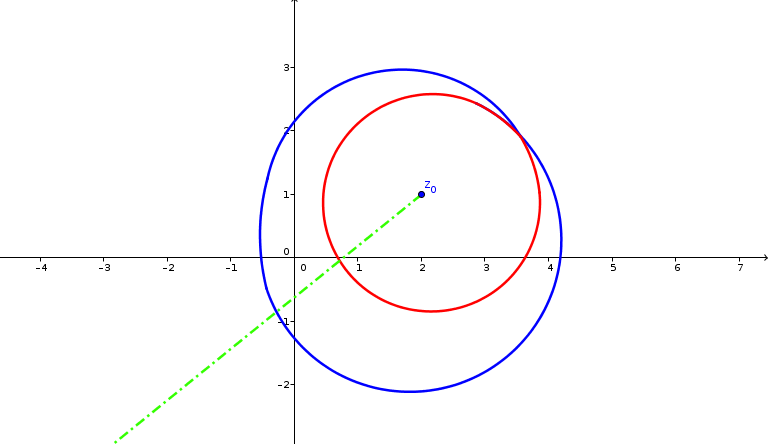
\includegraphics[width=0.75 \textwidth]{immagini/indice.png}
\end{figure}
\begin{teorema}
Sia $f$ una funzione continua sul dominio D. Sono equivalenti le seguenti affermazioni:
\begin{enumerate}
\item $\int_{z_1}^{z_2} f(z)dz$ non dipende dal cammino $\gamma$ che unisce $z_1$ a $z_2$ in $\C$
\item $\exists \, \int_{\gamma} f(z)dz \, \forall$ cammino chiuso $\gamma$ in D (differenziabile con continuità a tratti)
\item $\exists$ una primitiva $F$ (funzione olomorfa su D tale che $F'=f$ su D)
\end{enumerate}
\end{teorema}
\begin{proof}
E' banale dimostrare le implicazioni $1) \implies 2)$ e $3) \implies 1),2)$. Dimostriamo l'implicazione $1) \implies 3)$.\\Chiamiamo $F(z)=\int_{z_0}^{z} f(z')dz'$; valutiamo $F(z+h)=F(z)+\int_{z}^{z+h} f(z')dz'$, dove $h\in \C$. \\Parametrizzando il segmento, otteniamo:
$$\gamma(t)=z+th \text{ e } \dot{\gamma}(t)=h$$
$$F(z+h)=F(z)+h \int_{0}^{1} f(z+th)dt \implies$$
$$\implies \frac{F(z+h)-F(z)}{h}-f(z)=\int_{0}^{1} f(z+th)dt-f(z)=\int_{0}^{1} f(z+th)-f(z)dt$$
Sappiamo che $\forall \, \epsilon >0 \, \exists \, \delta_{\epsilon}: \, |f(z+h)-f(z)|<\epsilon \, \forall \, h: \, |h|<\delta_{\epsilon}$; quindi:
$$\left|\frac{F(z+h)-F(z)}{h}-f(z)\right| = \left|\int_{0}^{1} f(z+th)-f(z)dt\right| \leq \int_{0}^{1} |f(z+th)-f(z)|dt \leq \epsilon $$
La frazione al primo membro della prima equazione tende a $f(z)$ per $h \to 0$, cioè la prima frazione va a 0; dato che la seconda diseguaglianza vale $\forall \, \epsilon > 0$, abbiamo la tesi.
\end{proof}

La funzione inversione $\frac{1}{z}$  è una funzione olomorfa su $\C \backslash \{0\}$; la sua primitiva è il logaritmo principale $Log(z)$, che è olomorfa su $\C \backslash \{(x;0) \, : \, x<0\}$. \\ Data una curva chiusa $\gamma$, abbiamo visto la funzione indice $Ind(\gamma,z)=\frac{1}{2i \pi} \int_{\gamma} \frac{dz'}{z'-z}$ che restituisce il numero di avvolgimenti della curva intorno al punto $z$ ($\notin \gamma$); se la curva circonda $z$, attraverserà il taglio, altrimenti la funzione diventa semplicemente l'integrale lungo una curva chiusa (che dà come risultato 0). Operativamente, basta contare gli attraversamenti del taglio da parte della curva $\gamma$: possiamo avere attraversamenti ''dall'alto verso il basso'' e ''dal basso verso l'alto''; i primi corrispondono ad avvolgimenti antiorari, il cui contributo è di $2i \pi$ (+1 per la funzione indice), i secondi ad avvolgimenti in senso antiorario, il cui contributo è $-2i \pi$ (-1 per la funzione indice). \\ La richiesta che il punto z non appartenga alla curva è dovuta al fatto che non è definito l'indice di un punto su una curva.
\\
Introduciamo ora un importante teorema, il teorema di Cauchy-Goursat:

\begin{teorema}(di Cauchy-Goursat)\\Sia $f$ una funzione olomorfa su un dominio $\mathcal{D}$; sia $\mathfrak{R}$ un rettangolo contenuto in $\mathcal{D}$; allora:
$$\int_{\partial \mathfrak{R}} f(z)dz=0$$
\end{teorema}
\begin{proof}
Dividiamo il rettangolo $\mathfrak{R}$ in quattro sottorettangoli che ereditano l'orientazione del bordo dal rettangolo di partenza; chiameremo questi quattro rettangoli prima generazione di rettangoli. Valutando l'integrale sulla frontiera di questi rettangoli, notiamo che i contributi sui lati in comune si annullano a vicenda, perchè l'orientazione è opposta; possiamo quindi scrivere:
$$\mathcal{I}=\int_{\partial \mathfrak{R}} f(z)dz=\sum_{i=1} ^4 \int_{\partial \mathfrak{R}_{1i}} f(z)dz$$
$$|\mathcal{I}| \leq \sum_{i=1} ^4 \left|\int_{\partial \mathfrak{R}_{1i}} f(z)dz \right| \leq 4|\mathcal{I}_1|$$ dove $\mathcal{I}_1$ è il rettangolo che ha modulo di valore massimo; dividendo questo rettangolo in altri quattro rettangoli e iterando le precedenti operazioni, otteniamo:
$$|\mathcal{I}| \leq 4|\mathcal{I}_1| \leq 4 \sum_{i=1} ^4\left|\int_{\partial \mathfrak{R}_{2i}} f(z)dz \right| \leq 4^2|\mathcal{I}_2| \leq \dots \leq 4^n |\mathcal{I}_n|$$
\\
Sia $L$ la diagonale del rettangolo $\mathfrak{R}$; quando dividiamo il rettangolo, la diagonale del rettangolo di generazione $n$ risulta essere $\frac{L}{2^n}$. \\ Abbiamo che $\mathfrak{R} \supset \mathfrak{R}_1 \supset \mathfrak{R}_2 \supset \dots \supset \mathfrak{R}_n$; per $n \to +\infty$, si ha che  $A_{\mathfrak{R}_n} \to 0$. \\Per un teorema dovuto a Cantor, sappiamo che esiste un punto $a$ tale che $\bigcap_{k=1} ^{+ \infty} \mathfrak{R}_k =\{a\}$.\\$f$ è una funzione olomorfa; allora possiamo scrivere $\frac{f(z)-f(a)}{z-a}$ attraverso la somma $f'(a)+r(z,a)$, dove $r(z,a)$ è tale che $|r(z,a)| \to 0$ quando $z \to a$. Quindi l'integrale calcolato sul rettangolo $\mathcal{I}_n$ (cioè il rettangolo avente area maggiore fra quelli di $n$-esima generazione) risulta essere:
$$\mathcal{I}_n= \int_{\partial \mathfrak{R}_n} f(z)dz = \int_{\partial \mathfrak{R}_n} [f(a)+f'(a)(z-a) + r(z,a)(z-a)]dz$$ A questo punto, dividiamo l'integrale secondo le somme; ci si accorge  che i primi due membri hanno contributi nulli, perchè sia $f(a)$ sia $(z-a)$ hanno primitiva e, dato che stiamo integrando su un cammino chiuso, per il teorema precedente abbiamo che l'integrale è nullo. Rimane quindi solo l'ultimo membro; passando ai moduli, otteniamo:
$$|\mathcal{I}_n|\leq \int_{\partial \mathfrak{R}_n} |r(z,a)| \, |(z-a)| \, dz \leq \epsilon \frac{L}{2^n} \, 4 \frac{L}{2^n}$$ dove $4 \frac{L}{2^n}$ maggiora il cammino; sostituendo nella relazione $|\mathcal{I}|=4^n |\mathcal{I}_n|$, otteniamo che $|\mathcal{I}| \leq 4 L^2 \epsilon$ e, per l'arbitrarietà di $\epsilon$, abbiamo dimostrato la tesi.
\end{proof}
\begin{teorema}
Sia $f$ una funzione continua su un dominio $\mathcal{D}$ e olomorfa su $\mathcal{D} \backslash \{a\}$; sia $\mathfrak{R}$ un rettangolo contenuto in $\mathcal{D}$; allora vale ancora il teorema dei rettangoli, cioè $\int_{\partial \mathfrak{R}} f(z)dz=0$.
\end{teorema}
\begin{proof}
Se il punto è all'interno del rettangolo, lo isoliamo con delle strisce verticali e orizzontali; è evidente che possiamo scrivere il rettangolo $\mathfrak{R}$ come la somma dei rettangoli $\mathfrak{R}_i$, e vale ancora la legge di cancellazione dei tratti in comune; quindi $\mathcal{I}=\sum_i \int_{\partial \mathfrak{R}_i} f(z)dz$. \\ Di questa sommatoria sopravvive soltanto il rettangolino contenente il punto $a$, cioè $\mathcal{I}=\int_{\partial \mathfrak{r}} f(z)dz$. A questo punto, possiamo scrivere che $|\mathcal{I}| \leq \sup_{z \in \mathfrak{r}} |f(z)| L(\mathfrak{r})$, dove $L(\mathfrak{r})$ è il perimetro del rettangolino. \\ Giocando sul fatto che possiamo prendere il rettangolo $\mathfrak{r}$ piccolo a piacere, facciamo tendere a zero il perimetro e quindi otteniamo la tesi.\\Se invece il punto è sul bordo, procediamo in maniera analoga; cambia solo la ''divisione'' del rettangolo (in questo caso, avremo che una delle due strisce è a ridosso del lato al quale appartiene $a$).
\end{proof}
\chapter{Funzioni intere}

Adesso parleremo di funzioni intere, cioè funzioni olomorfe su tutto il piano, questo mi permette di costruire facilmente la primitiva. \\ Sia $F(z)=\int_0 ^{Re(z)} f(x)dx + i \int_0 ^{Im(z)} f(Re(z)+ iy)dy$, cioè il percorso rosso:

\begin{figure}[h!]
  \centering
    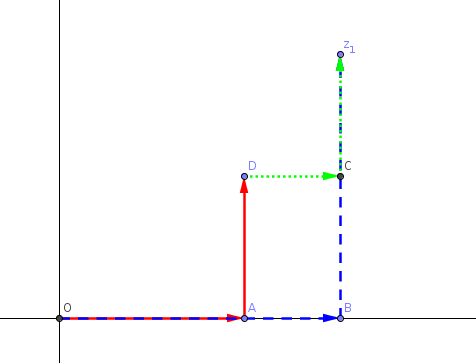
\includegraphics[width=0.5\textwidth]{immagini/percorsi-integrale.png}
\end{figure}

Adesso invece valutiamo $F(z_1)=F(z+h)$ con $h \in \C$; sulla falsa riga dell'esempio precedente, seguiamo il percorso blu ottenendo:
$$F(z+h)=\int_O ^B f(z)dz + \int_B ^{z+h} f(z')dz'$$
Applicando il teorema dei rettangoli a $\mathfrak{R}_{ABCD}$, otteniamo che la somma degli integrali sui lati del rettangolo è nulla, cioè $\int_A ^B f(z)dz+\int_B ^C f(z)dz+\int_C ^D f(z)dz+\int_D ^A f(z)dz=0$; quindi possiamo affermare che  $\int_A ^B f(z)dz+\int_B ^C f(z)dz=\int_C ^D -f(z)dz+\int_A ^D f(z)dz$. Sostituendo nella formula precedente, otteniamo che $F(z+h)=F(z)+\int_{z \to C \to z+h} f(z')dz'$.

A questo punto, facciamo in modo che sia a destra sia a sinistra appaia un rapporto incrementale; definito $\varphi$ il cammino $z \to C \to z+h$, la nostra equazione diventa:
$$\frac{F(z+h)-F(z)}{h}-f(z)=\frac{1}{h} \int_{\varphi}f(z')dz' -  f(z)\frac{1}{h} \int_{\varphi}dz'$$
dove è facile dimostrare che $f(z)=f(z)\frac{1}{h} \int_{\varphi}dz'$, perchè si ha che $\int_{\varphi}dz'=h$, e dunque: 
$$\frac{1}{h} \int_{\varphi}dz'=\frac{h}{h}=1$$

Utilizzando le proprietà dell'integrale, abbiamo che:
$$\frac{F(z+h)-F(z)}{h}-f(z)=\frac{1}{h} \int_{\varphi}[f(z')-f(z)]dz'$$
Passando ai moduli :
$$\left|\frac{F(z+h)-F(z)}{h}-f(z)\right|=\left|\frac{1}{h} \int_{\varphi}[f(z')-f(z)]dz'\right| \leq \frac{1}{|h|} \sup_{z \in \varphi} |f(z')-f(z)| (|Re(h)|+|Im(h)|)$$
Per la continuità di $f(z)$, abbiamo che $|f(z')-f(z)| < \epsilon$ e per le proprietà dei numeri complessi $|Re(h)|+|Im(h)| \leq 2|h|$; quindi otteniamo:
$$\left|\frac{F(z+h)-F(z)}{h}-f(z)\right|<2 \epsilon$$
Quindi, per $h \to 0$, si ha che $|F'(z)-f(z)|< \epsilon$, cioè $F'(z)=f(z)$; abbiamo quindi dimostrato che una funzione intera ammette primitiva.
\\
Da questa dimostrazione discende un importante teorema, il teorema di Cauchy.
\begin{teorema}
sia $f(z)$ una funzione intera e $\gamma$ un cammino chiuso; allora l'integrale di f su $\gamma$ ha valore nullo, cioè $\oint_{\gamma} f(z)dz=0$.
\end{teorema}
\section{La formula di Cauchy}

Sia $f$ una funzione intera; definiamo inoltre la funzione ausiliaria:
$$g(z)=\left\{  \begin{array}{l l}    \frac{f(z)-f(z_0)}{z-z_0} & \quad z \neq z_0\\    f'(z_0) & \quad z=z_0  \end{array} \right.$$
La funzione $g(z)$ è olomorfa ovunque tranne che in $z_0$ (cioè è olomorfa su $\C \backslash \{z_0\}$) ed è continua su tutto $\C$. Data una curva chiusa $\gamma$, con $z_0 \notin \gamma$, per le proprietà dell'integrale abbiamo che $0= \oint_{\gamma} g(z') dz'=\oint_{\gamma} \frac{f(z')-f(z_0)}{z'-z_0} dz'$. Dividendo per $2 \pi i$ otteniamo la cosiddetta formula integrale di Cauchy:
$$\oint_{\gamma} \frac{f(z')-f(z_0)}{z'-z_0} \frac{dz'}{2 \pi i} =f(z_0) Ind(\gamma, z_0)$$
Questa funzione mi permette, conoscendone i valori sulla curva $\gamma$, di conoscere i valori della funzione stessa all'interno della curva.

Sia ad esempio $\gamma$ la circonferenza centrata in $z_0$ e di raggio $\rho$; una possibile parametrizzazione è $z(\theta)=z_0 + \rho e^{i\theta}$. Inserendo nella formula ricavata precedentemente la variabile $z(\theta)$, e ricordando che il differenziale cambia ($dz=i \rho e^{i\theta}d\theta$), otteniamo:
$$i \rho  \int_0 ^{2 \pi} \frac{e^{i\theta}}{2 i \pi} \frac{f(z_0+ \rho e^{i \theta})}{ \rho  e^{i\theta}} d\theta=f(z_0)$$
Un corollario importante alla formula integrale di Cauchy è il teorema della media:
\begin{teorema}
Il valore di una funzione intera $f(z)$ al centro di una circonferenza $C_{\rho} (z_0)$ è uguale alla media (sugli angoli) dei punti sul bordo della circonferenza.
$$f(z_0)=\frac{1}{2 \pi} \int_0 ^{2 \pi} f(z_0 +  \rho e^{i\theta}) d\theta$$
\end{teorema}
\begin{corollario}
Il modulo di una funzione intera non ha picchi, cioè $|f(z_0)| \leq \sup_{|z-z_0| \leq  \rho } |f(z)|$
\end{corollario}
\begin{teorema} (di Liouville)\\
Sia $f$ una funzione intera tale che $|f(z)| \leq M$, con M finito. allora $f$ è una funzione costante. (Oppure: una funzione intera, a meno che non è costante, non è limitata in modulo).
\end{teorema}
\begin{proof}
Sfruttando la formula integrale di Cauchy, abbiamo che 
$$f(z)-f(0)=\int_{\gamma} \frac{f(z')}{z'-z} \frac{dz'}{2 \pi i}-\int_{\gamma} \frac{f(z')}{z'-0} \frac{dz'}{2 \pi i}=\int_{\gamma} \frac{z}{(z'-z)z} f(z') \frac{dz'}{2 \pi i}$$
Prendiamo come curva la circonferenza centrata nell'origine e di raggio $\rho$ tale che $|z| \leq \rho$; parametrizziamo la circonferenza come al solito: $z'=\rho e^{i\theta}$ (e quindi $dz'=i \rho e^{i\theta} d\theta$). Sostituendo nell'equazione precedente, otteniamo che:
$$f(z)-f(0)=i \rho z \int f(\rho e^{i\theta}) \frac{1}{(\rho e^{i\theta}-z)\rho e^{i\theta}} \frac{e^{i\theta}}{2 i \pi} d\theta$$
e, passando ai moduli:
$$|f(z)-f(0)|=|z| \, \left|\int f(\rho e^{i\theta}) \frac{1}{(\rho e^{i\theta}-z)\rho e^{i\theta}} \frac{e^{i\theta}}{2 i \pi} d\theta \right| \leq$$
$$\leq |z|\sup_{\theta \in [0;2\pi]} \frac{|f(\rho e^{i\theta})|}{|\rho e^{i\theta}-z|} \frac{L(\gamma)}{2 \pi} \leq$$
$$\leq |z| M \sup_{\theta \in [0;2\pi]} \frac{1}{|\rho e^{i\theta}-z|} =M \frac {|z|}{\rho-|z|}$$
Dato che possiamo prendere la circonferenza grande a piacere, mandiamo $\rho$ a $+\infty$ e quindi otteniamo che $|f(z)-f(0)| \leq 0$, ma allora, dato che il modulo è una quantità positiva, abbiamo che $|f(z)-f(0)|=0$, e quindi $f(z)=f(0)$.

\end{proof}
\begin{corollario}
Sia $f$ una funzione intera; se la funzione si annulla per $z \to \infty$, allora $f \equiv 0$.
\end{corollario}
\begin{corollario}
Se $f = \sum \alpha z^n$ per $z \to \infty$, allora $f(z)$ è un polinomio di grado $n$.
\end{corollario}
\begin{teorema} (di Picard)\\
Sia $f$ intera. Se $f(z) \neq a$ e $f(z) \neq b$, allora $f$ è costante.
\end{teorema}
Quindi l'immagine di una funzione intera è tutto il piano complesso tranne al più un punto, altrimenti la funzione è una funzione costante.
\begin{teorema} (Teorema fondamentale dell'algebra)\\
Sia $p(z)$ un polinomio di grado $n$; tale polinomio possiede almeno uno zero.
\end{teorema}
La dimostrazione di questo teorema è sufficiente per dimostrare la fattorizzazione di un polinomio.
\begin{proof}
Per assurdo, sia $p(z) \neq 0$ $\forall z$; allora $\frac{1}{p(z)}$ è intero, e si ha che $\frac{1}{p(z)} \to 0$ per $z \to 0$; infatti, dato che $p(z) \neq 0$, non può essere diverso da un'altro valore (per il teorema di Picard) e quindi $p(z)$ non è limitato. Ma allora, per il teorema di Liouville, si ha che $\frac{1}{p(z)}=0$ ovunque. il che è contro l'ipotesi di partenza. Abbiamo quindi dimostrato la tesi.
\end{proof}

Introduciamo ora la formula di fattorizzazione, che si rivelerà molto utile per il calcolo degli integrali:
\begin{equation}
p(z)=\sum_{k=1} ^n \frac{1}{p'(z_k)} \frac{1}{z-z_k}
\end{equation}
Sia ora $p(z)$ un polinomio e $\gamma$ un cammino chiuso. Il valore di $\oint_{\gamma} \frac{p'(z)}{p(z)-c} \frac{dz}{2 i \pi} $ mi dà il numero di soluzioni dell'equazione $p(z)=c$ chiuse dalla curva $\gamma$ (contate con la loro molteplicità algebrica). Come lo vediamo? \\ Chiamiamo $q(z)=p(z)-C$; tale polinomio è tale che $q'(z)=p'(z)$. sostituendo all'interno dell'integrale, otteniamo:
$$\oint_{\gamma} \frac{q'(z)}{q(z)} \frac{dz}{2 i \pi}=\oint_{\gamma} \sum_{k=1} ^n \frac{1}{z-z_k} \frac{dz}{2 i \pi}$$
dove i $z_k$ sono gli zeri di $q(z)$.
Quindi abbiamo una somma funzioni indice, cioè $\sum_k Ind(\gamma,z_k)$.

Prendiamo una funzione f continua su $\C$. Diciamo che f è doppiamente periodica se $\exists w_1,w_2 \in \C$, con $w_1 \neq \lambda w_2$ (per $\lambda \in \R$) tali che $f(z+w_1)=f(z)=f(z+w_2)$ $\forall z$, oppure in alternativa, tali che $f(z+n_1w_1+n_2w_2)=f(z)$ $\forall n_2, n_2 \in \Z$, $\forall z \in \C$.
\begin{teorema} (di Dixon)\\
Sia $\mathcal{D}$ aperto e connesso, $\gamma$ cammino differenziabile con continuità  a tratti, $Ind(\gamma,z)=0$ $\forall z \in \mathcal{D}$, f funzione olomorfa su $\mathcal{D}$. Allora valgono le formule delle funzioni intere, cioè:
$$\int_{\gamma} f(z') dz'=0 \text{ e } \int_{\gamma} \frac{f(z')}{z-z'} \frac{dz'}{2 \pi i}=f(z) Ind(\gamma,z)$$
con $z \notin \gamma$.
\end{teorema}
Vale anche il teorema inverso:
\begin{teorema} (di Morera)\\
Se l'integrale di Cauchy di una funzione continua si annulla per tutti i cammini chiusi (differenziabili con continuità a tratti) in un dominio limitato $\mathcal{D}$, allora $f$ è olomorfa su $\mathcal{D}$.
\end{teorema}

\section{La funzione Gamma di Eulero}

La funzione Gamma di Eulero è definita come:

\begin{equation}
\Gamma (z)= \int_0 ^{\infty} e^{-s} s^{z-1} ds
\end{equation}
dove s è un numero complesso; questo ci permette di riscrivere $\Gamma (z)$ come:
$$\Gamma (z)=\int_0 ^{\infty} e^{-s} s^{x-1} e^{iy log(s)} ds$$
In questo modo, risulta ovvio che:
$$|\Gamma (z)| \leq \int_0 ^{\infty} e^{-s} s^{x-1} ds = \Gamma (Re(z))$$
Quindi si ha che in $Re(z)>0$ la funzione $\Gamma(z)$ è olomorfa. Le principali proprietà della Gamma di Eulero sono:
\begin{itemize}
\item $\int_{\gamma} \Gamma (z) dz=\int_{\gamma} dz \int_0 ^{\infty} e^{-s} s^{z-1} ds= \int_0 ^{\infty} e^{-s} \int_{\gamma} e^{(z-1)log(s)} dz ds=0$
\item $\Gamma (x+1) = x \Gamma (x)$
\item $\Gamma (1)=1$ e, per induzione, $\Gamma (n+1)=n!$
\item $\Gamma (\frac{1}{2}) = \sqrt{\pi}$
\item $\Gamma (n+ \frac{1}{2})= \frac{2n-1}{2} \Gamma (\frac{1}{2})= \frac{(2n-1)}{2} \sqrt{\pi}$
\end{itemize}


\chapter{Serie}

\section{Serie numeriche}

Come nel campo dei reali, la serie numerica è scritta come $\sum_{i=0} ^{\infty} a_i$ con $a_i \in \C$; definita la successione delle somme parziali $S_n=\sum_{i=0} ^n a_i$, recuperiamo tutte le informazioni sulla convergenza già viste in altri ambiti:
\begin{teorema} (Criterio di convergenza secondo Cauchy)\\$S_n$ converge $\iff$ $S_n$ è di Cauchy, cioè se $\forall \epsilon >0 \exists N_{\epsilon}$ : $|S_{m+n} - s_m| < \epsilon$ $\forall m>N_{\epsilon}, \forall n>0$
\end{teorema}
La condizione che $|S_{m+n} - s_m| < \epsilon$ equivale a chiedere che $\left|\sum_{i=m+1} ^{m+n} a_i \right| < \epsilon$. \\Osserviamo che la condizione necessaria per la convergenza è che il termine generale (in modulo) vada a zero (questo perchè le formule sopra valgono $\forall m,n$). Oltretutto, abbiamo che $\left|\sum_{i=m+1} ^{m+n} a_i \right| \leq \sum_{i=m+1} ^{m+n} |a_i|$; definiamo quindi la \textbf{convergenza assoluta}, cioè la convergenza della serie dei moduli.
\begin{teorema}
Se una serie converge assolutamente, allora converge, cioè 
$$\sum |a_i|<\infty \implies \sum a_i<\infty$$
\end{teorema}
I criteri per la convergenza assoluta sono:
\begin{itemize}
\item Criterio del confronto:	$|a_i|<b_i$ $\forall i$ e $\sum b_i$ converge $\implies \sum a_i$ converge
\item Criterio della radice:		$\limsup_i \sqrt[i] {|a_i|} <1 \implies \sum a_i$ converge
\item Criterio del rapporto:		$\limsup_i \frac{a_{i+1}}{a_i}<1 \implies \sum a_i$ converge
\end{itemize}
	Sia nel caso del criterio del confronto sia nel caso del criterio della radice, nel momento in cui esiste il limite normale non dobbiamo scomodale il lim sup, ma possiamo ricorrere al limite semplice.

\section{Serie geometrica}

La serie geometrica è una serie della forma $\sum_{n=0} ^{\infty} z^n$; di questa serie sappiamo calcolare il valore effettivo della somma; infatti si ha che $S_n=1+z+z^2+z^3+ \dots +z^n$ e $S_{n+1}=S_n + z^{n+1}$; quindi si ha che $z \, S_n=S_{n+1} -1$ e, sostituendo le relazioni precedentemente ricavate, si ottiene che $S_n=\frac{1-z^{n+1}}{1-z}$. Da quì è facile osservare che la convergenza di $S_n$ dipende dal valore di z, cioè che $S_n$ converge se $|z|<1$; valutando la serie per $n \to \infty$ si ha che $\sum_{n=0} ^{\infty} z^n=\frac{1}{1-z}$, con $|z|<1$.
\\Esempi:
\begin{itemize}
\item $e^z =e^x e^{iy}=e^x (cos(y)+i sen(y))$ \\$e^z=\sum \frac{z^n}{n!}$ converge assolutamente su $\C$
\item $\sum \frac{1}{n^z} = \zeta(z)$: la funzione Zeta di Riemann converge se $Re(z)>1$
\end{itemize}

\section{Serie di funzioni}

Consideriamo la successione di funzioni $\{f_k\}$ con $f_k:E \to \C$ (dove E non deve per forza essere un sottoinsieme di $\C$); cosa sono la convergenza puntuale e la convergenza uniforme? \\La convergenza puntuale in un punto $p \in E$ si rivela essere la solita condizione di Cauchy:

$$\forall \epsilon >0 \, \, \exists N_{\epsilon, p} \text{ : } |f_n(p) -f_m(p)| < \epsilon \, \, \forall n,m>N_{\epsilon, p}$$ 
Per quanto riguarda la convergenza uniforme, invece, l'indice N non dipende dal punto p:
$$\forall \epsilon >0 \,\, \forall p \in E \, \, \exists N_{\epsilon} \text{ : } |f_n(p) -f_m(p)| < \epsilon \, \, \forall n,m>N_{\epsilon}$$
Consideriamo ora la successione delle somme parziali $S_n(p)=\sum_{k=0} ^{\infty} f_k(p)$; $S_n$ converge uniformemente su E se $\forall \epsilon >0 \, \, \forall p \in E \, \, \exists N_{\epsilon}$ : $|\sum_{k=m+1} ^{m+n} f_k(p)| < \epsilon$ $\forall m>N_{\epsilon}, \forall n>0$.
\\Vediamo ora una condizione sufficiente per la convergenza uniforme:
\begin{teorema} (Criterio M di Weierstrass)\\
Se $\exists b_k>0$ : $|f_k(p)|<b_k$ $\forall p \in E$, con $\sum_k b_k$ convergente $\implies \sum_k f_k(p)$ converge.
\end{teorema}
D'ora in avanti, parleremo di funzioni in cui il dominio $D \in \C$, cioè funzioni $f_k:D \subset \C \to \C$.
\begin{teorema}
Sia data una serie $\sum_{k=0} ^{\infty} f_k(z)$ convergente su $D \in \C$ e sia $\gamma$ un cammino differenziabile a tratti in D. Allora 
$$\int_{\gamma} \sum_{k=0} ^{\infty} f_k(z) dz=\sum_{k=0} ^{\infty} \int_{\gamma} f_k(z) dz$$
\end{teorema}

\begin{proof}
Definiamo la funzione $S_n(z)=\sum_{k=0} ^n f_k(z)$; sappiamo che ogni $S_n$ è continua, perchè somma di funzioni continue. Oltre ciò, ho (per ipotesi) che $S_n$ converge uniformemente su D ad un limite $S$, e in particolare lo farà sul compatto $\gamma$. \footnote{Parliamo di $\gamma$ come compatto perchè il cammino $\gamma:[a;b] \to \C$ parametrizzato rappresenta un compatto.} Allora $S$ è continua su $\gamma$, cioè esiste $\int_{\gamma} S(z) dz
$. \\Calcoliamo $\left|\sum_{k=0} ^n \int_{\gamma} f_k(z)dz - \int_{\gamma} \sum_{k=0} ^n f_k(z)dz \right| =$\footnote{Dato che abbiamo una somma finita, possiamo portare il simbolo di sommatoria dentro il primo integrale.}$\left|\int_{\gamma} [S_n(z)-S(z)]dz \right| \leq L[\gamma] \epsilon$; infatti si ha che $\forall \epsilon >0$ $\exists N$ : $|S_n-S|<\epsilon$ $\forall n>N$. \\Dato che vale per ogni $\epsilon$, si ha che $\sum_{k=0} ^n \int_{\gamma} f_k(z)dz=\int_{\gamma} \sum_{k=0} ^n f_k(z)dz$.

\end{proof}
Definiamo ora la \textbf{convergenza normale} di una serie di funzioni complesse:
\begin{definizione}
Una serie di funzioni $f_k:D \subset \C \to \C$ converge normalmente se:
\begin{itemize}
\item Converge puntualmente $\forall p \in D$
\item $\forall p$ esiste un disco chiuso dove la serie converge uniformemente
\end{itemize}
\end{definizione}
Attraverso la convergenza normale possiamo dare una dimostrazione alternativa del teorema precedente.

\section{Serie di potenze}

Una serie di potenze è una serie di funzioni della forma:

\begin{equation}
\sum_{k=0} ^{\infty} c_k (z-a)^k, \, c_k \in \C
\end{equation}
Il punto a è detto \textbf{centro della serie}.

\begin{teorema} (di Abel-Weierstrass)
\\Se la serie di potenze $\sum_{k=0} ^{\infty} c_k (z-a)^k$ converge per $z=z_0$, allora:

\begin{enumerate}
\item La serie converge assolutamente $\forall z$ nel disco aperto $|z-a|<|z_0-a|$
\item La serie converge uniformemente su ogni disco chiuso di raggio $|z_0-a|(1- \eta)$, con $\eta \in (0;1)$
\end{enumerate}
\end{teorema}
\begin{proof}
Dimostriamo i due punti separatamente:
\begin{enumerate}
\item Dato che la serie converge in $z_0$, si ha che $\exists N$ : $|c_k||z_0-a|^k<1$ $\forall k>N$. Da questo, ricaviamo che $|c_k| < \frac{1}{|z_0-a|^k}$; quindi, possiamo scrivere che $|c_k(z-a)^k|= |c_k||z-a|^k<\left|\frac{z-a}{z_0-a}\right|^k$. Allora si ha che $\sum_{k=0} ^{\infty} c_k (z-a)^k$ converge assolutamente, poichè si ha che $\sum_{k=0} ^{\infty} |c_k (z-a)^k|<$ $<\sum_{k=0} ^{\infty} \left|\frac{z-a}{z_0-a}\right|^k$, la quale converge purchè $\left|\frac{z-a}{z_0-a}\right|<1$, cioè $|z-a|<|z_0-a|$.
\item Poniamo su $z$ la condizione che $|z-a|\leq |z_0-a|(1-\eta)$; per quanto visto nel punto precedente, abbiamo visto che esiste un $N$ tale che $\forall k>N$ si ha che $\left|c_k(z-a)^k\right| \leq \frac{1}{|z_0-a|^k} |z-a|^k \leq$ $\leq  \frac{1}{|z_0-a|^k} |z_0-a|^k (1-\eta)^k=(1-\eta)^k$ e si ha che $\sum_k (1-\eta)^k$ converge.
\end{enumerate}

\end{proof}
Cosa può succedere alla convergenza di una serie di potenze? Grazie a questo teorema, possiamo esprimere tre possibili casi:
\begin{itemize}
\item La serie converge solo per $z=a$
\item La serie converge su tutto $\C$ (o comunque in tutto l'insieme di definizione)
\item La serie non converge ovunque, ma converge in almeno un punto $z_0 \neq a$
\end{itemize}
In quest'ultimo caso, andiamo a definire una zona del piano complesso in cui la serie converge; tale area è rappresentata dal raggio di convergenza (che, nel caso in cui la serie non converga ovunque, è finito).

\section{Raggio di convergenza di una serie}

\begin{teorema} (Criterio di Cauchy-Hadamard)\\
La serie $\sum_k |c_k(z-a)^k|$ converge se $\limsup_k \sqrt[k]{|c_k(z-a)^k|} <1$.
\end{teorema}
Otteniamo che $\frac{1}{|z-a|} > \limsup_k \sqrt[k]{|c_k|} \equiv \frac{1}{R}$; quindi si ha $|z-a|=R$ e $\limsup_k \sqrt[k]{|c_k|} = R^{-1}$.
\begin{teorema}	

Sia $f$ una funzione olomorfa su D. Sia $D(a,r)$ un disco di raggio r centrato in a, contenuto in $D$ con contorno $C(a,r)$ \footnote{Circonferenza centrata in a e di raggio r.}. Si ha che:
$$\forall z \in D(a,r)\text{ }f(z)=\sum_{k=0} ^{\infty} c_k (z-a)^k\text{, con }c_K= \int_{C(a,r)} \frac{f(z)}{(z-a)^{k+1}} \frac{dz}{2 i \pi}$$
cioè, per ogni punto z appartenente al disco $D(a,r)$ la funzione $f$ può essere riscritta sottoforma di serie di potenze, co n i coefficienti $c_k$ ben definiti.
\end{teorema}
\begin{proof}
Partiamo dalla formula integrale di Cauchy applicata a $f(z)$; abbiamo che $f(z)=\int_{C(a,r)} \frac{f(s)}{s-z} \frac{ds}{2 i \pi}$. \\Riscriviamo $\frac{1}{s-z}$ come $\frac{1}{(s-a)-(z-a)}=\frac{1}{s-a} \frac{1}{1-\frac{z-a}{s-a}}= \sum_{n=0} ^{\infty} (\frac{z-a}{s-a})^n$; sostituiamo la serie all'interno dell'integrale, e otteniamo che:
$$f(z)=\int_{C(a,r)} \frac{f(s)}{s-a} \sum_{n=0} ^{\infty} \left(\frac{z-a}{s-a}\right)^n \frac{ds}{2 i \pi}=\footnote{Dato che la serie converge uniformemente, possiamo portare la sommatoria fuori dall'integrale.} \sum_{n=0} ^{\infty} (z-a)^n \int_{C(a,r)} a\frac{f(s)}{(s-a)^{n+1}} \frac{ds}{2 i \pi}$$
che è la costruzione dettata dal teorema.
 
 \end{proof}

\subsection{Prodotto di cauchy di due serie di potenze con centro in a=0}

Siano date due serie $\sum_{k=0} ^{\infty} a_k$ e $\sum_{l=0} ^{\infty} c_l$; definiamo il \textbf{prodotto di Cauchy} delle due serie è la serie $\sum_{m=0} ^{\infty} \sum_{k=0} ^m a_k c_{m-k}$. \\Similmente, date due serie di potenze $\sum_{k=0} ^{\infty} a_k z^k$ e $\sum_{l=0} ^{\infty} c_l z^l$, il prodotto di Cauchy delle due serie di potenze è $\sum_{m=0} ^{\infty} z^m \sum_{k=0} ^m a_k c_{m-k}$. 

Notiamo che se delle due serie una converge assolutamente e l'altra converge semplicemente (o puntualmente), allora il prodotto di Cauchy converge semplicemente (o puntualmente), mentre se entrambe convergono assolutamente allora anche il prodotto di Cauchy converge assolutamente.
\\
Quando abbiamo una singolarità e vogliamo sviluppare la funzione in serie di potenze, tale serie convergerà in un disco di raggio al più uguale al minimo fra le distanze fra il centro della serie e i punti in cui ho singolarità.
\\
Esempi:
\begin{itemize}
\item Sia data la funzione $f(z)=\frac{1}{(z-1)(z-3)}$; gli sviluppi in serie centrati nei punti A e C convergono nei due dischi riportati.
\begin{figure}[h!]
  \centering
    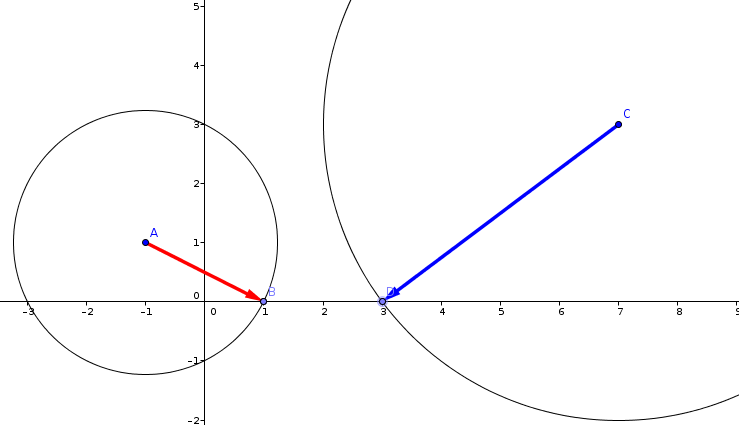
\includegraphics[width=0.5\textwidth]{immagini/frazione-polinomio-2.png}
\end{figure}
\item Sia data la funzione logaritmo principale; i dischi di convergenza delle serie risultano essere delle due tipologie riportate in figura:
\begin{figure}[h!]
  \centering
    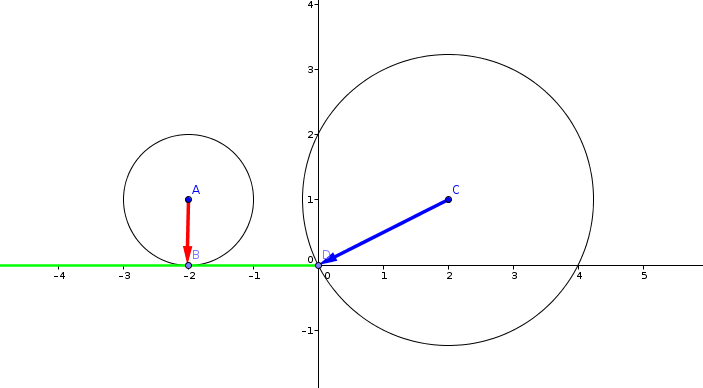
\includegraphics[width=0.5\textwidth]{immagini/logaritmo-2.png}
\end{figure}
\end{itemize}
Vediamo ora in che rapporto stanno la derivata di una serie e la serie di partenza:
\begin{teorema}
La serie $S(z)=\sum_{n=0} ^{\infty} c_n (z-a)^n$ e la sua serie derivata $S'(z)=\sum_{n=1} ^{\infty} n c_n (z-a)^{n-1}$ hanno lo stesso raggio di convergenza, cioè convegono sullo stesso disco aperto.
\end{teorema}

Sia $f$ una funzione olomorfa in un dominio $\mathbb{D}$, con $f(z)=\sum_{n=0} ^{\infty} c_n (z-a)^n$ nel disco aperto $D(a,r) \subset \mathbb{D}$. Abbiamo visto che i coefficienti $c_n$ sono da $\oint_{C(a,r)} \frac{f(z)}{(z-a)^{n+1}} \frac{dz}{2 i \pi}$; oltretutto, per $z \in \mathbb{D}$, grazie alla formula integrale di Cauchy abbiamo che:
$$f(z)=\oint_{C(a,r)} \frac{f(z')}{z'-z} \frac{dz'}{2 i \pi}$$
che, valutato in $z=a$, ci dà $c_0$, cioè $c_0=f(a)$. 
\clearpage
Similmente, abbiamo che
$$f'(z)=\oint_{C(a,r)} \frac{f(z')}{(z-z')^1} \frac{dz'}{2 i \pi}$$
che, valutato in $z=a$, ci dà $c_1=f'(a)$. Procedendo in tale maniera, otteniamo che i coefficienti $c_n$ sono dati dalla formula:
$$c_n=\frac{f^{(n)}(a)}{n!}=\oint_{C(a,r)} \frac{f(z)}{z-a} \frac{dz}{2 i \pi}$$

\section{Polinomi di Hermite}

Sia $H(z,x)=e^{-z^2+2xz}$ una funzione intera per ogni $x \in \R$ (ma lo è anche per $x \in \C$). Prendiamone lo sviluppo in serie di potenze centrato in $z=0$:
\begin{equation}
H(0,x)= \sum_{n=0} ^{\infty} z^n \frac{H_n(x)}{n!}
\end{equation}
Viene definita un'intera famiglia di funzioni $H_n$ a partire da un'unica funzione $H(z,x)$; tale funzione è detta \textbf{funzione generatrice} (dei \textbf{polinomi di hermite}). Grazie a quanto visto per le serie di potenze, dato che i vari $ \frac{H_n(x)}{n!}$ rappresentano i coefficienti $c_n$ della serie, ricaviamo che 
$$\frac{H_n(x)}{n!}=\oint \frac{H(z,x)}{z^{n+1}} \frac{dz}{2 i \pi}=\oint \frac{e^{-z^2+2xz}}{z^{n+1}} \frac{dz}{2 i \pi}$$
Sviluppando in serie l'esponenziale, otteniamo che 
$$ \frac{H_n(x)}{n!}=\sum_{l=0} ^{\infty} \frac{(2x)^l}{l!} \oint e^{-z^2} z^{l-n-1} \frac{dz}{2 i \pi}$$
Se $l-n-1 \geq 0$, allora $e^{-z^2} z^{l-n-1}$ è una funzione intera e quindi, per il teorema di Cauchy, l'integrale si annulla; questo fa sì che la somma sulle $l$ diventi una somma finita, poichè l'integrale è nullo se $l \geq n+1$. Otteniamo dunque che:
$$\frac{H_n(x)}{n!}=\sum_{l=0} ^n \frac{(2x)^l}{l!} \oint \frac{e^{-z^2}}{z^{n+1-l}} \frac{dz}{2 i \pi}$$
cioè $H_n(x)$ è un polinomio di grado n. Oltretutto abbiamo che 
$$ \oint \frac{e^{-z^2}}{z^{n-l+1}} \frac{dz}{2 i \pi}=\frac{1}{(n-l)!} \frac{\partial^{n-l}}{\partial z^{n-l}} \left[e^{-z^2} \right]_{z=0}$$
Allora si ha che 
$$H_n(x)=\sum_{l=0} ^n \frac{n!}{(n-l)!} \frac{(2x)^l}{l!} \frac{\partial^{n-l}}{\partial z^{n-l}} \left[e^{-z^2} \right]_{z=0}=\footnote{Definiamo un nuovo indice $k=n-l$; tale indice va da 0 a n.}\sum_{k=0} ^n \frac{n!}{k!(n-k)!} (2x)^{n-k} \frac{\partial^k}{\partial z^k} \left[e^{-z^2} \right]_{z=0}$$
%\end{alertenv}
Dato che lo sviluppo in serie di $e^{-z^{2}}$  contiene solo le derivare pari, operiamo un'altrocambio di esponente $k=2j$; in questo modo, lo sviluppo diventa:
$$H_n(x)=\dots=\sum_{j=0} ^{\lfloor \frac{n}{2}\rfloor}\frac{n!}{(2j)!(n-2j)!} (2x)^{n-2j} \frac{\partial^{2j}}{\partial z^{2j}} \left[e^{-z^2} \right]_{z=0}=$$
$$=\sum_{j=0} ^{\lfloor \frac{n}{2}\rfloor}\frac{n!}{(2j)!(n-2j)!} (2x)^{n-2j}(-1)^j \frac{(2j)!}{j!}=\sum_{j=0} ^{\lfloor \frac{n}{2}\rfloor}\frac{(-1)^j n!}{j!(n-2j)!} (2x)^{n-2j}$$
Tale polinomio è detto \textbf{polinomio di Hermite}; il termine dominante in un polinomio di Hermite di grado n è $2^n x^n$. Il fatto che gli esponenti 
dei vari membri del polinomio siano dati da $n-2j$ mi permette di conservare la parità degli esponenti, cioè vale che $H_n(-x)=(-1)^n H_n(x)$; infatti, mandando $z \to -z$ e $x \to -x$ otteniamo che $\sum_{n=0} ^{\infty} z^n \frac{H_n(x)}{n!}=\sum_{n=0} ^{\infty} (-z)^n \frac{H_n(-x)}{n!}$ che ci dà proprio la relazione scritta prima. \\
Altre due relazioni importanti sono:
\begin{itemize}
\item $\partial_x H(z,x)=2zH(z,x)$. Grazie alla derivazione per le serie abbiamo che: $$\sum_{n=0} ^{\infty} \frac{z^n}{n!}H_n'(x)=2\sum_{n=0} ^{\infty} z^{n+1} \frac{H_n(x)}{n!}=2\sum_{n=1} ^{\infty} z^n \frac{H_{n-1}(x)}{(n-1)!}$$
da cui si ricava che $H_n'(x)=2nH_{n-1}(x)$.
\item $\partial_z H(z,x)=(-2z+2x)H(z,x)$. Procedendo come prima, si ricava che $H_{n+1}(x)=2xH_n(x) -2nH_{n-1}(x)$.\\Quindi i polinomi di Hermite soddisfano un'equazione di ricorrenza; ricavati i primi due polinomi, possiamo ricavare tutti gli altri a cascata grazie a questa formula.
\end{itemize}

\section{Prolungamento analitico}

Iniziamo introducendo due proprietà delle funzioni olomorfe:
\begin{teorema}
Gli zeri di una funzione olomorfa (non identicamente nulla) sono punti isolati.
\end{teorema}
\begin{proof}
Sia $f$ una funzione olomorfa, e $a$ un punto tale che $f(a)=0$; quindi possiamo scrivere $f$ nella forma $f(z)=c(z-a)^k \varphi (z)$, dove $c \neq 0$ e $k$ è l'ordine dello zero in $a$. La funzione $\varphi (z)$ invece sarà della forma $1+c_1 (z-a) \dots$, cioè è una funzione olomorfa tale che $\varphi (a)=1$.\\In un disco $D(a,r)$ contenuto nel dominio abbiamo che la $\varphi (z)$ è continua, e in particolare è continua nel punto $a$; quindi vale la definizione di continuità.\\
Poniamo $\epsilon = \frac{1}{2}$; per la continuità, si ha che 
$$\exists \rho : |\varphi (z) -1|<\frac{1}{2} \, \, \forall z \, : \, |z-a| < \rho$$
Ma allora $\varphi (z) \neq 0$ nel disco $|z-a| < \rho$; quindi lo zero è un punto isolato.

\end{proof}
\begin{teorema}
Se una funzione $f$ olomorfa su annulla su un insieme di punti contenente un punto di accumulazione del dominio, allora $f$ è nulla nel dominio.
\end{teorema}
Questo teorema ci permette di mutuare alcune formule viste nel campo reale; ad esempio:
\begin{itemize}
\item Nei reali vale che $sen(2x)=2sen(x)cos(x)$; dimostriamo che vale anche nei reali. \\Scriviamo $sen(2z)-2sen(z)cos(z)$; essa è una funzione intera e si annulla per $z \in \R$. Dato che si annulla in tale insieme di punti, si annulla ovunque, cioè $sen(2z)=2sen(z)cos(z)$.
\item Sia data la funzione $\Gamma(z)=\int_0 ^{\infty} dt e^{-t} t^{z-1}$; tale funzione è olomorfa sul semipiano complesso $Re(z)>0$. oltretutto, sul semiasse reale positivo, vale che $\Gamma(x+1)=x\Gamma(x)$ e $\Gamma(n+1)=n!$. Queste relazioni valgono anche per un qualsiasi z complesso? Come per il caso precedente, abbiamo che la differenza dei due membri di ciascuna equazione valutata nel campo complesso è una funzione olomorfa e si annulla lungo il semiasse reale, cioè è identicamente nulla, e quindi le due relazioni valgono anche nel semipiano complesso $Re(z)>0$.
\end{itemize}

Possiamo ora introdurre la nozione di prolungamento analitico:
\begin{definizione}
Siano $f$ e $\tilde{f}$ due funzioni olomorfe rispettivamente sui domini $D$ e $\tilde{D}$ tali che $D \subset \tilde{D}$. se le due funzioni coincidono su $D$, allora la funzione $\tilde{f}$ si dice \textbf{prolungamento analitico} di $f$ da $D$ a $\tilde{D}$.
\end{definizione}
\begin{teorema}
Il prolungamento analitico $\tilde{f}$ su $\tilde{D}$ è unico.
\end{teorema}
\begin{proof}
Sia il dominio $D$ tale che contenga un punto di accumulazione di $\tilde{D}$; per assurdo, si ipotizzi l'esistenza di due prolungamenti analitici $\tilde{f}$ e $\tilde{\tilde{f}}$ da $D$ a $\tilde{D}$. Esse devono essere tali che $\tilde{f}=f=\tilde{\tilde{f}}$ in $D$; ma allora si ha che $\tilde{f}-\tilde{\tilde{f}}=0$ in $D$, cioè  $\tilde{f}-\tilde{\tilde{f}}=0$ in $\tilde{D}$.

\end{proof}
Un esempio di prolungamento analitico lo si può trovare nelle serie di potenze:

Sia $f(z)=\sum_n c_n (z-a)^n$ lo sviluppo in serie di Taylor centrato in a di una funzione; esso converge assolutamente nel disco $D(a,r)$. Preso un'altro punto $\tilde{a}$, possiamo costruire lo sviluppo in serie di Taylor centrato in $\tilde{a}$, che risulta essere $\tilde{f}(z)=\sum_n \tilde{c_n} (z-\tilde{a})^n$, che convergerà assulatemente sul disco $D(\tilde{a},\tilde{r})$. \\E' facile osservare che i due sviluppi devono essere uguali sull'intersezione dei due dischi; quindi, la funzione
$$F(z)=\left\{  \begin{array}{l l}    f(z) & \quad \text{su } D\\    \tilde{f}(z) & \quad \text{su } \tilde{D}  \end{array} \right.$$
è una funzione olomorfa su $D \cup \tilde{D}$.

Un'utile applicazione è quella di estendere la funzione Gamma di Eulero all'insieme $\C \backslash \Z^-$; infatti, abbiamo che:
$$\Gamma(z)=\int_0 ^{\infty} dt \, e^{-t} t^{z-1}=\int_0 ^{1} dt \, e^{-t} t^{z-1} + \int_1 ^{\infty} dt \, e^{-t} t^{z-1} =\footnote{Qui abbiamo che il secondo addendo è una funzione intera, quindi ci riduciamo a operare solo sul primo membro}$$
$$=\int_0 ^{1} dt \, \left(\sum_n \frac{(-1)^n}{n!} \right) t^{z-1+n} + \int_1 ^{\infty} dt \, e^{-t} t^{z-1}=\frac{1}{z+n}$$
Nel semipiano $Re(z)>0$ la $\Gamma(z)$ e il suo prolungamento analitico assumono gli stessi valori; i punti esclusi rappresentano dei poli semplici.
\\
\\
Beta di Eulero...
\\
\\
\section{Equazione di Weber}

L'equazione di Weber è un'equazione del tipo
\begin{equation}
-u'' + x^2 u = \lambda u
\end{equation}
Siamo capaci di trovare una soluzione a questa equazione differenziale di secondo grado, cioè $u_0(x)=e^{\frac{1}{2} x^2}$; derivando e sostituendo, vediamo che $u_0$ soddisfa l'equazione di Weber per $\lambda=1$.

Proviamo a generalizzare, prendendo come soluzione  $u(x)=e^{\frac{1}{2} x^2} H(x)$. Derivando e sostituendo, si ottiene
$$-H''(x)+2xH(x)=(\lambda -1)H(x)$$
Come possiamo risolvere l'equazione? utilizzando la tecnica degli sviluppi in serie, scriviamo
$$H(x)=\sum_{l=0} ^{\infty} c_l x^l$$
\begin{osservazione}
C'è un teorema\footnote{Non ci è dato sapere di quale teorema si tratta...} che ci dice che, avendo un'equazione differenziale del tipo $u''+pu'+qu=0$, dove $p$ e $q$ sono delle funzioni della variabile $x$ (come la $u$) tali che esse siano olomorfe su un insieme comune, allora se scrivo $u$ sottoforma di serie di potenze, il suo raggio di convergenza sarà pari al minoredei raggi di convergenza degli sviluppi in serie di potenze di $p$ e $q$. Questo fatto ci permette di studiare la serie nelò suo insieme di convergenza.
\end{osservazione}
Derivando e sostituendo, otteniamo:
$$-\sum_{l=0} ^{\infty} l(l-1)c_l x^{l-2} +2\sum_{l=0} ^{\infty} l c_l x^{l-1} =(\lambda -1) \sum_{l=0} ^{\infty} c_l x^l$$
$$\sum_{l=0} ^{\infty} \left[-(l+2)(l+1)c_{l+2} + 2l c_l - (\lambda -1) c_l  \right]x^l=0$$
Otteniamo quindi un'equazione di ricorrenza:
$$c_{l+2} =\frac{2l - \lambda +1}{(l+2)(l+1)} c_l$$
Questa salta un termine ad ogni passo; in questo modo abbiamo delle soluzioni pari, generate dalla combinazione $c_0 \neq 0$ e $c_1=0$, e delle soluzioni dispari, generate dalla combinazione $c_0=0$ e $c_1 \neq 0$. 
Nel caso in cui $\lambda=2n+1$, $H(x)$ è un polinomio di grado $n$. In questo caso l'equazione diventa:
$$H_n''(x) +2xH_n'(x)=2nH_n(x)$$
che è un'equazione differenziale risolta dal polinomio di Hermite di grado n.

Possiamo quindi riscrivere le equazioni di ricorrenza come:
$$(l+2)! c_{l+2} = (2l - \lambda +1) l! c_l$$
cioè, ponendo $d_l=l! c_l$:
$$d_{l+2} = (2l - \lambda +1) d_l$$
che, quando $\lambda = 2n +1$, diventa:
$$d_{l+2} = -2(n - \lambda) d_l$$
Quindi scriviamo le equazioni:
$$-u_n'' + x^2 u_n = (2n+1)u_n$$
$$-u_m'' + x^2 u_m = (2m+1)u_m$$
dove $u_k=e^{-\frac{1}{2} x^2}H_k(x)$; moltiplicando le due equazioni rispettivamente per $u_m$ e $u_n$ e sottraendole membro a membro, otteniamo:
$$-(u_n'' u_m - u_m'' u_n)=2(n-m)u_n u_m$$
dove abbiamo che
$$-(u_n'' u_m - u_m'' u_n)=-\frac{d}{dx}[u_n' u_m - u_m' u_n]$$
che si annulla poichè ho delle esponenziali negative (infatti gli $u_k$ hanno la forma di una gaussiana non normalizzata). Quindi, integrando da $- \infty$ a $+ \infty$, otteniamo:
$$0=2(n-m)u_n u_m=2(n-m) \int_{-\infty} ^{+\infty} dx \, e^{-x^2} H_n(x) H_m(x)$$
Ricaviamo quindi una condizione di ortogonalità fra le funzioni; infatti, per $n \neq m$, abbiamo che:
$$\int_{-\infty} ^{+\infty} dx \, u_n(x) u_m(x) \iff \int_{-\infty} ^{+\infty} dx \, e^{-x^2} H_n(x) H_m(x)\footnote{Si ricorda che le $x$ sono indici discreti, le $u_k$ sono funzioni di Hermite e gli $H_k$ sono i polinomi di Hermite.} $$ 

\section{Serie di Laurient}
Prendiamo la funzione $f=\frac{1}{z-a}$; vogliamo fare uno sviluppo in serie di potenze centrato in $z_0$; scriviamo:
$$\frac{1}{z-a} = \frac{1}{(z-z_0) -(a-z_0)} = \frac{(-1)}{a-z_0} \frac{1}{1- \frac{z-z_0}{a-z_0}} = \frac{(-1)}{a-z_0} \sum_{l=0} ^{\infty} \left( \frac{z-z_0}{a-z_0} \right) ^l$$
Questa serie vive nel disco centrato in $z_0$ e raggio $|z_0 .a|$ (cioè la distanza dalla singolarità più vicina). \\Allo stesso modo, possiamo scrivere:
$$\frac{1}{z-a} = \frac{1}{z-z_0} \frac{1}{1- \frac{a-z_0}{z-z_0}} =\sum_{l=0} ^{\infty} \frac{(a-z_0)^l}{(z-z_0)^{l+1}}$$
che è una serie di potenze che converge al di fuori del disco definito in precedenza.

Introduciamo quindi un nuovo tipo di serie, la \textbf{serie di Laurent} che differisce dalle solite serie per il fatto che l'indice, invece di variare in $\N$, varia in $\Z$. Le serie di Laurent sono della forma:
$$\sum_{n=-\infty} ^{+\infty} c_n (z-a)^n$$
 dove il punto $a$ rappresenta il centro della serie. \\ Possiamo scomporre la serie di Laurent in due serie classiche; infatti si ha che:
 $$\sum_{n=-\infty} ^{+\infty} c_n (z-a)^n=\sum_{n=0} ^{+\infty} c_n (z-a)^n + \sum_{n=1} ^{+\infty} c_{-n} \frac{1}{(z-a)^n}$$
La serie di Laurent risulta essere ''ben posta'' se convergono separatamente le due serie; la prima serie converge all'interno del disco $D(a,R)$, dove $R=\frac{1}{\limsup \sqrt[n]{|c_n|}}$, mentre la seconda, come visto nell'esempio precedente, converge esternamente al disco $D(a,r)$, dove $r=\limsup \sqrt[n]{|c_{-n}|}$. L'intersezione dei due insiemi di convergenza mi restituisce un \textbf{anello di convergenza} (cioè entro il quale la serie di Laurent converge) della forma $r<|z-a|<R$; notiamo che, poichè la serie di Laurent converga, deve essere verificato che $r<R$, altrimenti l'insieme scritto non ha senso.
\\Chiameremo la prima delle due serie in cui abbiamo scomposto la serie iniziale \textbf{parte analitica} mentre la seconda (cioè quella con indici di segno cambiato) \textbf{parte principale}.

Diamo adesso i criteri secondo i quali una funzione è sviluppabile in serie di Laurent in un dato insieme:
\begin{teorema}
Sia $f$ una funzione olomorfa nell'anello $r<|z-a|<R$. Allora $f$ ammette sviluppo in serie di Laurent in tale anello, cioè
$$f(z)=\sum_{n=-\infty} ^{+\infty} c_n (z-a)^n \text{ dove } c_n= \oint_{\gamma} \frac{dz}{2 \pi i} \frac{f(z)}{(z-a)^{n+1}}$$
con $\gamma$ che rappresenta un qualsiasi cammino chiuso contenuto nell'anello di convergenza. Tale sviluppo è unico.
\end{teorema}
\begin{proof}
Sia $z \in A$, dove $A$ è l'anello $r<|z-a|<R$; costruiamo un cammino chiuso che contenga $z$ e che giri in senso antiorario intorno ad esso; chiamiamo $C$ tale cammino chiuso.
\begin{figure}[h!]
  \centering
    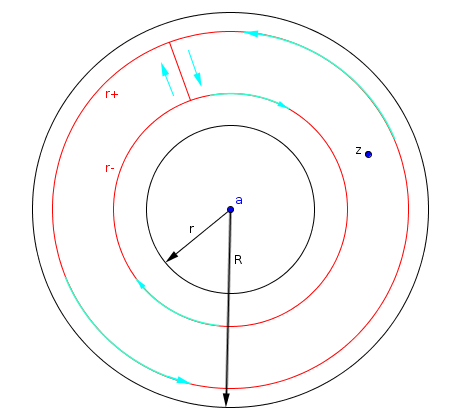
\includegraphics[width=0.4\textwidth]{immagini/teorema_laurent.png}
\end{figure}
Grazie alla formula integrale di Cauchy, sappiamo che  $\oint_C \frac{dz'}{2 \pi i} \frac{f(z')}{z-z'}$; possiamo vedere il cammino $C$ come somma di quattro cammini:
$$C=C(r+) \cup C(r-) \cup \text{ segmento percorso due volte in sensi opposti}$$
Si nota subito che il contributo del segmento è nullo, poichè viene percorso prima in un verso e poi nell'altro, e quindi i due contributi si annullano a vicenda. \\
Sostituendo tale cammino, l'integrale di Cauchy diventa:
$$\oint_{C(r+)} \frac{dz'}{2 \pi i} \frac{f(z')}{z-z'} - \oint_{C(r-)} \frac{dz'}{2 \pi i} \frac{f(z')}{z-z'}$$
dove il segno ''-'' davanti al secondo integrale mi permette di cambiare il verso di percorrenza della circonferenza $C(r-)$, in modo tale che entrambe le circonferenze siano percorse in senso antiorario.\\
Ora riscriviamo $\frac{1}{z-z'}$ come:
$$\frac{1}{(z'-a)-(z-a)}=\left\{  \begin{array}{l l}    \frac{1}{z'-a} \frac{1}{1-\frac{z-a}{z'-a}}=\sum_{l=0} ^{\infty} \frac{(z-a)^l}{(z'-a)^{l+1}} & \quad z' \in C(r+)\\    -\frac{1}{z-a} \frac{1}{1-\frac{z'-a}{z-a}}=-\sum_{l=0} ^{\infty} \frac{(z'-a)^l}{(z-a)^{l+1}} & \quad z' \in C(r-)  \end{array} \right.$$
Sostituiamo quindi gli sviluppi in serie geometrica negli integrali di prima e otteniamo:
$$f(z)=\oint_{C(r+)} \frac{dz'}{2 \pi i} f(z') \sum_{l=0} ^{\infty} \frac{(z-a)^l}{(z'-a)^{l+1}} - \oint_{C(r-)} \frac{dz'}{2 \pi i} f(z') \sum_{l=0} ^{\infty} \frac{(z'-a)^l}{(z-a)^{l+1}}=$$
$$=\sum_{l=0} ^{\infty} (z-a)^l \oint_{C(r+)} \frac{dz'}{2 \pi i} \frac{f(z')}{(z'-a)^{l+1}} - \sum_{l=0} ^{\infty} \frac{1}{(z-a)^{l+1}} \oint_{C(r-)} \frac{dz'}{2 \pi i} f(z') (z'-a)^l$$
dove abbiamo portato le sommatorie fuori dai rispettivi integrali poichè convergono uniformemente.\\
Dato che la funzione $f$ è olomorfa nell'anello $A$, possiamo sostituire i due cammini con altri cammini chiusi; oltretutto, dato che nell'integrale non compare $z$, tali cammini potranno attraversare quel punto. Otteniamo dunque che:
$$=\sum_{l=0} ^{\infty} (z-a)^l \oint_{\gamma} \frac{dz'}{2 \pi i} \frac{f(z')}{(z'-a)^{l+1}} - \sum_{l=0} ^{\infty} \frac{1}{(z-a)^{l+1}} \oint_{\gamma} \frac{dz'}{2 \pi i} f(z') (z'-a)^l$$
Cambiando indici nel secondo integrale (ponendo $m=l+1$), otteniamo lo sviluppo di Laurent.

Per quanto riguarda l'unicità, invece, supponiamo che esista un'altro sviluppo $\sum_{n=-\infty} ^{+\infty} \tilde{c_n} (z-a)^n$; mostriamo che $c_n=\tilde{c_n}$:
$$c_n= \oint_{\gamma} \frac{dz}{2 \pi i} \frac{f(z)}{(z-a)^{n+1}}= \oint_{\gamma} \frac{dz}{2 \pi i} \sum_{l=-\infty} ^{+\infty} \tilde{c_l} (z-a)^{l-n-1}= \footnote{Utilizziamo $l$ per indicare che stiamo guardando due sviluppi diversi.}$$
$$=\sum_{l=-\infty} ^{+\infty} \tilde{c_l} \oint_{\gamma} \frac{dz}{2 \pi i} (z-a)^{l-n-1}=\footnote{Ricordiamo che l'integrale vale 1 se $l-n-1=-1$, altrimenti è nullo} \sum_{l=-\infty} ^{+\infty} \tilde{c_l} \delta_{l-n-1,-1} = \tilde{c_n}$$

\end{proof}
Riportiamo alcuni esempi di sviluppi in serie di Laurent:
\begin{itemize}
\item Lo sviluppo in serie della funzione $f(z)=\frac{(z+1)^2}{z}$ è molto semplice da ottenere; infatti, basta  svolgere il quadrato al numeratore per ottenere tale sviluppo che risulta essere $z+2+\frac{1}{z}$, dove $z+2$ è la parte analitica mentre $\frac{1}{z}$ è la parte principale. Tale sviluppo in serie di Laurent è centrato in $z=0$ e vale sull'anello $0<z<\infty$; quando un anello è del tipo $0<z<a$, con $a>0$, viene detto \textbf{disco forato}.
%Nota: ricontrollare l'esempio qua sotto, perchè non sono sicuro sia giusto%
\item Sia data la funzione $f(z) = \frac{1}{z^2 (a-z)^2}$; dato che abbiamo due punti ''critici'', dobbiamo studiare le varie casistiche:
\begin{itemize}
\item Se $0<|z|<1$, possiamo scrivere uno sviluppo in serie di Laurent che convergerà nel disco forato centrato in $z=0$. Abbiamoche la funzione risulta essere:
$$\frac{1}{z^2} \frac{d}{dz} \left(\frac{1}{1-z} \right)=\footnote{Conosciamo il valore della somma della serie armonica semplice.} \frac{1}{z^2} \frac{d}{dz}(1+z+z^2+z^3+ \dots)= \frac{1}{z^2} \frac{d}{dz} \sum_{n=0} ^{\infty} z^n=$$
$$= \frac{1}{z^2} \sum_{n=0} ^{\infty} nz^{n-1}=\sum_{n=0} ^{\infty} nz^{n-3}=\frac{1}{z^2} + \frac{2}{z} + 3 + 4z + 5z^2 + \dots$$
dove la parte principale è $\frac{1}{z^2} + \frac{2}{z}$, mentre il resto compone la parte analitica.
\item Se invece andiamo a fare lo sviluppo di Laurent in $z=1$, avremo che in questo caso il disco di convergenza è $0<|z-1|<1$, cioè è il disco forato centrato in $z=1$. Otteniamo:
$$\frac{1}{z^2 (1-z)^2}=\frac{1}{(z-1)^2} \frac{1}{[1+(z-1)]^2}=\frac{1}{(z-1)^2} \sum_{n=0} ^{\infty} (-1)^n (z-1)^n=$$
$$= \frac{1}{(z-1)^2} \left(1-(z-1)+(z-1)^2-(z-1)^3+ \dots \right)=$$
$$=\frac{1}{(z-1)^2} - \frac{2}{(z-1)} + 3 - 4(z-1) + 5(z-1)^2 + \dots$$
dove la parte principale è $\frac{1}{(z-1)^2} - \frac{2}{(z-1)}$, mentre il resto forma la parte analitica.
\end{itemize}
\item Sia data la funzione $f(z)=e^{\frac{x}{2} (z- \frac{1}{z})}$; essa è una funzione olomorfa su $\C \backslash \{0\}$. Possiamo quindi sviluppare la funzione il serie di Laurent centrando tale sviluppo in $z=0$; otteniamo quindi uno sviluppo della forma:
$$\sum_{n=-\infty} ^{\infty} z^n J_n (x)$$
dove le $J_n(x)$ sono dette \textbf{funzioni di Bessel} con indice intero.
\end{itemize}

\chapter{Teoria dei residui}

Nel momento in cui lo sviluppo in serie di Laurent presenta una singolarità isolata, abbiamo una naturale classificazione delle singolarità.\\Ma procediamo per gradi: innanzitutto, diamo la definizione di singolarità isolata:
\begin{definizione}
Un punto $a \in \C$ è una \textbf{singolarità isolata} per la funzione $f$ se $f$ è olomorfa nel disco forato $D'(a,r)=D(a,r) \backslash \{a\}$ per un valore di $r>0$.
\end{definizione}
Una volta trovato sìffatto disco, possiamo scrivere lo sviluppo in serie di Laurent, ottenendo come già visto:
$$\sum_{n=-\infty} ^{+\infty} c_n (z-a)^n=\sum_{n=0} ^{+\infty} c_n (z-a)^n + \sum_{n=1} ^{+\infty} c_{-n} \frac{1}{(z-a)^n}$$
Possiamo osservare come la parte principale diverga per $z \to a$; a seconda di come è fatta la parte principale, classifichiamo le singolarità isolate nella seguente maniera:
\begin{itemize} 
\item La singolarità si dice \textbf{rimovibile} se i coefficienti $c_{-n}$ sono  nulli $\forall n \geq 1$ (cioè se la parte principale è nulla). Un esempio è la funzione $\frac{sen(z)}{z}$; infatti sviluppandola in $z=0$ otteniamo:
$$\frac{sen(z)}{z}= \frac{1}{z} \left(z-\frac{z^3}{3!} + \frac{z^5}{5!}+ \dots \right)=1-\frac{z^2}{3!} + \frac{z^4}{5!}+ \dots$$
cioè lo sviluppo non ha parte principale.
\item La singolarità si dice \textbf{polo di ordine n} se i coefficienti $c_{-n}$ sono definitivamente nulli, cioè se $c_{-n} \neq 0$ e $c_{-n-k}=0$ $\forall k \geq 1$. \\
Un esempio è la funzione $f(z)=\frac{1}{(z-3)^3}$, che coincide con il suo sviluppo in serie di Laurent centrato in $z=3$ e che risulta avere in tale punto un polo di ordine 3.
\item  La singolarità si dice \textbf{essenziale} se, diversamente dal polo di ordine n, i coefficienti della parte principale non sono definitivamente nulli, cioè se $\forall N>0$ $\exists k>N$ : $c_{-k} \neq 0$. \\ Un esempio è la funzione $f(z)=e^{\frac{1}{z}}$, il cui sviluppo di Laurent centrato in $z=0$ è:
$$\sum_{n=0} ^{\infty} \frac{1}{n!} \frac{1}{z^n}$$
cioè lo sviluppo ha solo parte principale.
\end{itemize}
%Nel caso di singolarità essenziale, non è definito il limite di $f(z)$ per $z \to a$; nel caso di polo di ordine n, tale limite è infinito; invece, nel caso di singolarità essenziale abbiamo che
\begin{definizione}
Una funzione si dice \textbf{meromorfa} su un domnio $\mathbb{D}$ se è olomorfa su $\mathbb{D}$ a meno di un insieme di singolarità isolate.
\end{definizione}
Concentriamoci ora sulla parte principale dello sviluppo in serie di Laurent di una funzione $f(x)$ con singolarità in $z=a$. Il coefficiente $c_{-1}$ dello sviluppo centrato in $z=0$ è detto \textbf{residuo} di $f$ in $z=a$ e si indica come:
$$c_{-1}=Res[f,a]=\oint_{\gamma} \frac{dz}{2 \pi i} f(z)$$
dove l'ultima uguaglianza e data dalla definizione dei coefficienti $c_n$ dello sviluppo di Laurent.
\\
Proviamo ad esempio a calcolare il residuo della funzione $f(z)=\frac{1}{z(z-1)}$, che presenta un polo semplice nei punti $z=0$ e $z=1$; abbiamo che:
\begin{itemize}
\item Nel disco forato $0<|z|<1$:
$$f(z)=\frac{1}{z} (-1) \sum_{n=0} ^{\infty} z^n = -\frac{1}{z} -1 -z-z^2- \dots$$
cioè $Res[f,0]=-1$.
\item Se invece scegliamo l'anello $|z|>1$:
$$f(z)= \frac{1}{z^2(1-\frac{1}{z})} = \frac{1}{z^2} \left[1+\frac {1}{z}+\frac{1}{z^2}+\dots \right]=\frac {1}{z^2}+\frac{1}{z^3}+\dots$$
cioè in questo caso si ha che $Res[f,0]=0$, poichè la singolarità non è essenziale; quindi, per poter classificare la singolarità, dobbiamo trovarci nel disco forato nel quale abbiamo tolto solo tale singolarità.
\end{itemize}

\section{Calcolo dei residui}
$$Res[f,a]=c_{-1}=\oint_{\gamma} \frac{dz}{2 \pi i} f(z)$$
A seconda del tipo di singolarità, il residuo ha valori diversi:
\begin{itemize}
\item Nel caso in cui la singolarità sia rimovibile, abbiamo che
$$Res[f,a]=0$$
\item Nel caso in cui la singolarità sia un polo semplice, lo sviluppo di Laurent centrato in $z=a$ é del tipo $f(z)=\frac{c_{-1}}{z-a}+c_0+c_1(z-a)+c_2(z-a)^2+ \dots$; quindi abbiamo che il coefficiente $c_{-1}$ può essere visto come:
$$c_{-1}=\lim_{z\to a} (z-a) f(z)$$
\item Nel caso in cui la singolarità sia un polo di ordine n, abbiamo che lo sviluppo di Laurent centrato in $z=a$ è del tipo:
$$f(z)=\frac{c_{-n}}{(z-a)^n}+ \dots + \frac{c_{-1}}{z-a}+c_0+c_1(z-a)+ \dots$$
Moltiplicando per $(z-a)^n$ otteniamo:
$$(z-a)^nf(z)=c_{-n}+ c_{n-1}+ \dots + c_{-1}(z-a)^{n-1}+c_0 (z-a)^n\dots$$
e si vede che, derivando ($n-1$)-volte l'espressione, eliminiamo tutti i coefficienti di ordine $k<-1$; oltretutto, dividiamo per $(n-1)!$, in modo tale che il coefficiente $c_{-1}$ rimanga isolato. Otteniamo dunque che:
$$\frac{1}{(n-1)!} \frac{d^{n-1}}{dz^{n-1}} [(z-a)^k f(z)]=c_{-1}+k c_0(z-a)+ \dots$$
e, passando al limite per $z \to a$, abbiamo il valore del residuo:
$$c_{-1}= \lim_{z \to a} \frac{1}{(n-1)!} \frac{d^{n-1}}{dz^{n-1}} [(z-a)^k f(z)]$$
\item Se la singolarità è essenziale, a meno di casi particolari, dobbiamo sempre ricondurci alla definizione dei coefficienti $c_{-1}$, cioè dobbiamo calcolarci $\oint_{\gamma} \frac{dz}{2 \pi i} f(z)$. \\Ad esempio, per calcolare il $Res[z^3 e^{\frac{1}{z}},0]$, dobbiamo calcolare $\oint_{\gamma} \frac{dz}{2 \pi i} z^3 e^{\frac{1}{z}}$; questo esempio è anche uno dei casi particolari in cui possiamo fare a meno di ricorrere alla definizione dei coefficienti della serie di Laurent: infatti, abbiamo che lo sviluppo di $z^3 e^{\frac{1}{z}}$ è:
$$f(z)=z^3 \sum_{n=0} ^{\infty} \frac{1}{k!} \frac{1}{z^k}=z^3+\frac{z^2}{2!}+\frac{z}{3!} +\frac{1}{4!} +\frac{1}{5!} \frac{1}{z} +\dots$$
cioè si ha che $Res[z^3 e^{\frac{1}{z}},0]=c_{-1}=\frac{1}{5!}$.
\end{itemize}
%Alcuni esempi
\begin{teorema} (Teorema dei Residui) \\
Sia $f$ una funzione olomorfa su un dominio $\mathbb{D} \backslash \mathcal{S}$, dove $\mathcal{S}$ è un'insieme di singolarità isolate di $f$ nel dominio $\mathbb{D}$; sia poi $\gamma$ un cammino chiuso contenuto in $\mathbb{D} \backslash \mathcal{S}$ tale che
$$Ind[\gamma,z]=0 \text{ se il punto } z \notin \mathbb{D}$$
Allora si ha che
$$\oint_{\gamma} f(z) dz = 2 \pi i \sum_{z_k \in \mathcal{S}} Res[f,z_k]\, Ind[\gamma,z_k]$$
\end{teorema}
Essenzialmente questo teorema ci permette di calcolare il valore di un integrale come somma dei residui di $f$ sulle sue singolarità, ma solo per quelle contenute nel dominio (da qui la richiesta che $Ind[\gamma,z]=0$ per i punti $z \notin \mathbb{D}$).
\\
\\
Vediamo ora la dimostrazione:
\begin{proof}
Per ogni singolarità isolata esiste un disco forato nel quale vale uno sviluppo di Laurent della forma:
$$f(z)=P_k(z)+A_k(z)$$
dove $P_k(z)$ e $A_k(z)$ sono dei polinomi che rappresentano rispettivamente la parte principale e la parte analitica dello sviluppo.\\
Costruiamo ora la funzione ausiliaria $g$ definita come:
$$g(z)=f(z)- \sum_k P_k(z)$$
Dimostriamo che questa funzione è olomorfa in $\mathbb{D}$. Per il teorema di Cauchy, si ha che $\oint_{\gamma} g(z)dz=0$; ma per definizione di $g$, abbiamo che $\oint_{\gamma} g(z)dz=\oint_{\gamma} f(z)dz - \sum_k \oint_{\gamma} P_k(z) dz$. \\
Per definizione, sappiamo che il termine $\oint_{\gamma} P_k(z) dz$ varrà $2 \pi i \, c_{-1} ^{(k)} Ind[\gamma,z_k]$ poichè , dato che la curva $\gamma$ non tocca nessuna singolarità, tutti i termini $\frac{c_{-n} ^{(k)}}{(z-z_k)^n}$ (con $n>1$) ammettono primitiva, e quindi il loro integrale su un cammino chiuso è nullo. Otteniamo quindi la tesi.

\end{proof}

Sia data la funzione $f(x)=\frac{1}{x^4+1}$; per calcolare l'integrale della funzione su tutto l'asse reale, ricorriamo al teorema dei residui; infatti, possiamo passare al campo complesso scrivendo:
$$\int_{-\infty} ^{+\infty} \frac{dx}{x^4+1}= \lim_{R \to \infty} \int_{-R} ^{+R} \frac{dx}{x^4+1}=\lim_{R \to \infty} \oint_{\gamma} \frac{dz}{z^4+1}$$
dove la curva $\gamma$ è quella rappresentata in figura sotto; si nota che l'ultimo passaggio è lecito perchè l'integrale sulla semicirconferenza si annulla per $R \to \infty$.
\begin{figure}[h!]
  \centering
    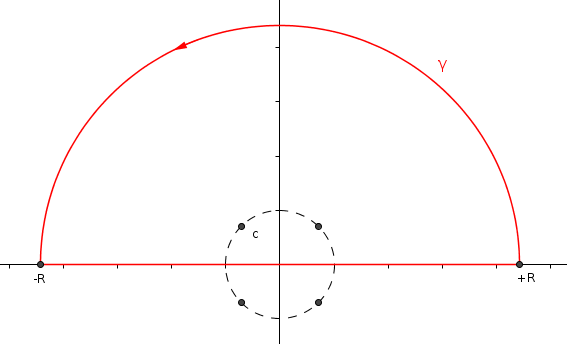
\includegraphics[width=0.5\textwidth]{immagini/esempio_residui.png}
\end{figure}
La funzione $f$ presenta quattro singolarità; esse sono tutti poli semplici e si trovano tutti sulla circonferenza unitaria.
Applicando quindi il teorema dei residui, abbiamo che:
$$ \oint_{\gamma} \frac{dz}{z^4+1}= 2 \pi i \left( Res \left[ \frac{1}{z^4+1}, e^{i \frac{\pi}{4}} \right] + Res \left[ \frac{1}{z^4+1}, e^{i \frac{3 \pi}{4}} \right] \right)$$
Calcoliamo i due residui separatamente:
$$Res \left[ \frac{1}{z^4+1}, e^{i \frac{\pi}{4}} \right]= \lim_{z \to e^{i \frac{\pi}{4}}} (z- e^{i \frac{\pi}{4}}) \frac{1}{z^4+1}=\footnote{Si ricorda che possiamo riscrivere $z^4+1$ come $(z-e^{i \frac{\pi}{4}})(z-e^{i \frac{3 \pi}{4}})(z-e^{i \frac{5 \pi}{4}})(z-e^{i \frac{7 \pi}{4}})$.}\lim_{z \to e^{i \frac{\pi}{4}}} \frac{1}{(z-e^{i \frac{3 \pi}{4}})(z-e^{i \frac{5 \pi}{4}})(z-e^{i \frac{7 \pi}{4}})}=$$
$$=\frac{1}{(e^{i \frac{\pi}{4}}-e^{i \frac{3 \pi}{4}})(e^{i \frac{\pi}{4}}-e^{i \frac{5 \pi}{4}})(e^{i \frac{\pi}{4}}-e^{i \frac{7 \pi}{4}})}=\frac{1}{e^{i \frac{3 \pi}{4}}} \frac{1}{(1-e^{i \frac{\pi}{2}})(1- e^{i \pi})(1- e^{i \frac{3 \pi}{2}})}=\frac{e^{-i \frac{3 \pi}{4}}}{(1-i)(2)(1+i)}=\frac{e^{-i \frac{3 \pi}{4}}}{4}$$
Allo stesso modo, calcoliamo $Res \left[\frac{1}{z^4+1}, e^{i \frac{3 \pi}{4}} \right]$, ottenendo:
$$Res\left[\frac{1}{z^4+1}, e^{i \frac{3 \pi}{4}} \right]= \dots =-\frac{e^{i \frac{3 \pi}{4}}}{4}$$
Adesso, risostituendo nella formula iniziale, otteniamo:
$$ \oint_{\gamma} \frac{dz}{z^4+1}= 2 \pi i \left(Res \left[ \frac{1}{z^4+1}, e^{i \frac{\pi}{4}} \right] + Res \left[ \frac{1}{z^4+1}, e^{i \frac{3 \pi}{4}} \right] \right)=2 \pi i \left(\frac{e^{-i \frac{3 \pi}{4}}}{4} -\frac{e^{i \frac{3 \pi}{4}}}{4} \right)=$$
$$=2 \pi i \left(\frac{1}{2} \frac{e^{-i \frac{3 \pi}{4}} - e^{i \frac{3 \pi}{4}}}{2} \right)=2 \pi i \left(\frac{1}{2} \left(-i \right) sen \left(\frac{3 \pi}{4} \right) \right)= \frac{\pi}{\sqrt{2}}$$
Quindi abbiamo ricavato il valore dell'integrale iniziale, cioè:
$$\int_{-\infty} ^{+\infty} \frac{dx}{x^4+1}=\frac{\pi}{\sqrt{2}}$$

\section{Gli integrali trigonometrici}

Il teorema dei residui può essere sfruttato per valutare degli integrali altrimenti di non facile determinazione, i cosìddetti \textbf{integrali trigonometrici}.
\\
\\
Calcoliamo ad esempio il valore di
$$\int_0 ^{2 \pi} \frac{cos(4 \theta)}{2+ cos \theta}d \theta$$
Abbiamo diversi metodi per calcolare tale integrale: possiamo sfruttarele proprietà trigonometriche per scrivere:
$$\int_0 ^{2 \pi} \frac{e^{i 4 \theta}+e^{-i 4 \theta}}{4+ e^{i \theta} + e^{-i \theta}}d \theta$$
ed effettuando un cambio di variabili:
$$\oint_{|z|=1} \frac{z^4 + \frac{1}{z^4}}{4+z+\frac{1}{z}} \frac{dz}{iz} = \oint_{|z|=1} \frac{z^4 + \frac{1}{z^4}}{4z+z^2+1} \frac{dz}{i}$$
Però in questo caso risulta ''scomodo'' il calcolo del polo di ordine 4.\\
Un'altra stradapossibile dopo aver ridotto l'integrale trigonometrico ad un integrale complesso è quella di porre prima $z=e^{i \theta}$ e poi $z=e^{-i \theta}$, cioè percorrere la circonferenza di raggio unitario prima in senso antiorario, poi in senso orario.
\\
\\
Possiamo aggirare i problemi derivanti dai precedenti due metodi considerando $Re[\int_0 ^{2 \pi} \frac{e^{i 4 \theta}}{2+ cos \theta}d \theta]$, che è ovviamente una riscrittura dell'integrale di partenza. Ponendo $z=e^{i \theta}$, l'integrale risulta:
$$\int_0 ^{2 \pi} \frac{cos(4 \theta)}{2+ cos \theta}d \theta=Re \left[\int_0 ^{2 \pi} \frac{e^{i 4 \theta}}{2+ cos \theta}d \theta \right]= Re \left[ \oint_{|z|=1} \frac{z^4}{2+\frac{z+\frac{1}{z}}{2}} \frac{dz}{iz} \right]=$$
$$=2Re \left[\oint_{|z|=1} \frac{z^4}{z^2+4z+1} \frac {dz}{i} \right]=\footnote{Gli zeri del denominatore sono $z_{1,2}=\frac{-4 \pm \sqrt{16-4}}{2}=-2 \pm \sqrt{3}$. Osseriviamo che solo $z_1$ si trova all'interno della circonferenza di raggio 1.} 2Re \left[\oint_{|z|=1} \frac{z^4}{(z-z_1)(z-z_2)} \frac {dz}{i} \right]=$$
$$=2Re \left[\frac{2 \pi i}{i}  \lim_{z \to z_1} (z-z_1) \frac{z^4}{(z-z_1)(z-z_2)} \right]=\frac{4 \pi z_1 ^4}{z_1-z_2}=4 \pi \frac{(\sqrt{3}-2)^4}{2 \sqrt{3}}$$
\\
\\
Quando viene richiesto di calcolare un'integrale su tutto l'asse reale, per poter passare agli integrali complessi (e quindi sfruttare il teorema dei residui) dobbiamo scegliere un cammino chiuso che sia equivalente a quello di partenza, cioè per il quale il contributo della ''linea di raccordo'' fra il semiasse positivo e il semiasse negativo (nel limite di $R \to \infty$) sia nullo. I percorsi che vengono solitamente scelti per comodità sono:
\begin{figure}[h!]
  \centering
    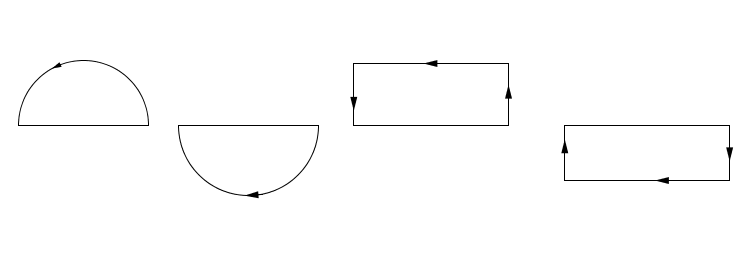
\includegraphics[width=0.8\textwidth]{immagini/percorsi_possibili.png}
\end{figure}
\\
Ad esempio per calcolare il valore dell'integrale $\int_{-\infty} ^{+\infty} dx f(x) \frac{e^{-ikz}}{\sqrt{2 \pi}}$ (la trasformata di Fourier della funzione $f$) abbiamo che, a seconda dei valori di $k$, dobbiamo scegliere percorsi diversi:
\begin{itemize}
\item Se $k>0$ scegliamo la semicirconferenza inferiore
\item Se $k<0$ scegliamo la semicirconferenza superiore
\end{itemize}
Questo è dovuto alla struttura dei numeri complessi; infatti, posto $z=x+iy$, abbiamo che:
$$e^{-ikz}=e^{-ik(x+iy)}=e^{-ik} e^{ky}$$
e quindi, per le richieste di annullamento del contributo della semicirconferenza, abbiamo i risultati citati sopra.
%Altri esempi
\begin{lemma} (di Jordan)\\
Se il contributo del semicerchio si annulla a $+\infty$, allora tale contributo è nullo.
\end{lemma}
Vediamo che questo fatto si verifica. Prendiamo $\int_{\cap} dz f(z) e^{ikz}$, con $k>0$ e $f$ continua; definiamo poi $M(r)=\sup_{\theta \in [0,\pi]} |f(r e^{i \theta})|$, dove abbiamo parametrizzato la circonferenza come $z=r e^{i \theta}$. Applicando la parametrizzazione anche all'integrale e prendendone il modulo, otteniamo:
$$\left|\int_{\cap} dz f(z) e^{ikz}\right|=\left|\int_0 ^{\pi} ird\theta f(r e^{i \theta}) e^{ikr(cos \theta + i sen \theta)}\right| \leq r \int_0 ^{\pi} d \theta |f(r e^{i \theta})| e^{-kr \, sen\theta} \leq$$
$$\leq r M(r) \int_0 ^{\pi} d \theta e^{-kr \, sen\theta} = 2 r M(r) \int_0 ^{\frac{\pi}{2}} d \theta e^{-kr \, sen\theta} \leq$$
$$\leq 2 r M(r) \int_0 ^{\frac{\pi}{2}} d \theta e^{-\frac{2kr}{\pi} \theta}=2rM(r) \frac{1-e^{-kr}}{\frac{2kr}{\pi}} \leq \frac{\pi}{k} M(r)$$
\begin{osservazione}
Nell'utilizzare il Lemma di Jordan dobbiamo stare attenti al segno di k; infatti, non è detto che valga anche per $k \leq 0$.
\end{osservazione}
%Altri esempi






%PRECEDENTE: teoria-residui
\chapter{Spazi di Hilbert e teoria degli operatori}

Sia $\H$ uno spazio lineare su $\C$, cioè uno spazio nel quale sono definite la somma e il prodotto per uno scalare. Esso si dice \textbf{spazio pre-hilbertiano} se è definito  il \textbf{prodotto interno}, cioè un'operazione $\H \times \H \to \C$ : $(x|x) \geq 0$, e $(x|x) =0 \iff x=0$.\\Quando scambiamo due termini nel prodotto interno così definito, prendiamo il complesso coniugato del nuovo prodotto, cioè si ha che $(x|y)=\overline{(y|x)}$.
\\
Il prodotto interno così definito è lineare nel secondo membro e antilineare nel primo; infatti:

\begin{itemize}
\item $(x|\lambda y_1 + \mu y_2)=(x|\lambda y_1) + (x|\mu y_2) =\lambda (x|y_1) + \mu (x|y_2)$
\item $(\lambda x_1+\mu x_2|y)=\overline{(y|\lambda x_1 + \mu x_2)}=\overline{\lambda (y|x_1)+ \mu (y|x_2)} = \overline{\lambda} (x_1|y) + \overline{\mu} (x_2|y)$
\end{itemize} Vediamo ora le proprietà del prodotto scalare:

\begin{itemize}
\item $x$ è ortogonale a $y$ ($x \perp y$) se $(x|y)=0$
\item Introduciamo la quantità $\|x\|=\sqrt{(x|x)}$, che dimostreremo essere la norma; risultano ovvie alcune proprietà:
\begin{itemize}
\item $\|x\| \geq 0$
\item $\|x\| =0 \iff x=0$
\item $\| \lambda x\|=|\lambda| \|x\|$
\end{itemize}
\item Prendiamo $x,y$ tali che $x \perp y$; si ha che $\|x+y\|^2=\|x\|^2+\|y\|^2$. Infatti: 
$$\|x+y\|^2=(x+y|x+y)=(x|x)+(x|y)+(y|x)+(y|y)=\|x\|^2+\|y\|^2$$
Questa uguaglianza risulta quindi essere il \textbf{teorema di Pitagora}.
\item $u_k$, con $k=1,2, \dots ,N$ è un \textbf{sistema ortonormale} di vettori di $\H$ se $(u_k|u_j)=\delta_{kj}$
\item \textbf{Disuguaglianza di Bessel}: $\|x\|^2 \geq \sum_{k=1} ^N |(u_k|x)|^2$ \\
Dimostriamo questo fatto: chiamiamo $x'=\sum_{k=1} ^N (u_k|x)u_k$, e scriviamo $x$ come $(x-x')+x'$. Mostriamo che $(x-x'|x')=0$; una volta mostrato questo, si ha che: 
$$\|x\|^2 =\|x+x'\|^2 + \|x'\|^2 \geq \|x'\|^2 =(x'|x')= \sum_{k=1} ^N (u_k|x)(x'|u_k)=$$
$$=\sum_{k=1} ^N (u_k|x)(x|u_k)=\sum_{k=1} ^N |(u_k|x)|^2$$
Infatti si ha che 
$$(x'|u_k)=(\sum_{l=1} ^N (u_l|x) u_l|u_k)=\sum_{l=1} ^N \overline{(u_l|x)} (u_l|u_k)=\sum_{l=1} ^N (x|u_l) \delta_{lk}=(x|u_k)$$
Possiamo dimostrarlo anche partendo dalla condizione $(x-x'|x') =0$; infatti:
$$(x-x'|x')=(x|x')-(x'|x')=\sum_{k=1} ^N (u_k|x)(x|u_k)-\|x'\|^2=0$$
e da qui si ottiene la disuaglianza di Bessel.
\item \textbf{Disuguaglianza di Schwarz}: $|(x|y)|\leq \|x\| \|y\|$ \\Siano $x,y,\lambda$ dei numeri complessi; per ogni $\lambda$ si ha che: 
$$0 \leq \|x+\lambda y\|^2=(x+\lambda y|x+\lambda y)=\|x\|^2+|\lambda|^2 \|y\|^2 + \overline{\lambda}(y|x) + \lambda (x|y) \leq \footnote{Si usa la proprietà dei numeri complessi per la quale $\overline{x} + x =2  Re(x) \leq 2|x|$.}$$
$$\leq \|x\|^2 +|\lambda|^2 \|y\|^2 +2|\lambda||(x|y)|$$
Possiamo vedere tale risultato come un'equazione quadratica nella variabile $|\lambda|$; cerchiamo la condizione $\Delta \leq 0$:
$$|(x|y)|^2 - \|x\|^2 \|y\|^2 \leq 0 \implies |(x|y)|^2 \leq \|x\|^2 \|y\|^2$$
Utilizzando tale relazione per maggiorare il risultato precendente e ponendo $\lambda=1$ otteniamo che:
$$\|x+y\|^2 \leq  \|x\|^2 + \|y\|^2 +2|(x|y)|^2 \leq \|x\|^2 +\|y\|^2+2\|x\|^2 \|y\|^2=(\|x\| + \|y\|)^2$$
e quindi $\|x+y\| \leq \|x\|+\|y\|$, cioè la tesi.
\end{itemize} Quindi $\|x\|=\sqrt{(x|x)}$ è una \textbf{norma (hilbertiana)}, poichè valgono le seguenti proprietà:

\begin{itemize}
\item $\|x\| \geq 0$, e $\|x\|=0 \iff x=0$
\item$\| \lambda x\|=| \lambda| \|x\|$
\item Vale una disuguaglianza triangolare, cioè la disuguaglianza di Schwarz
\end{itemize} Le proprietà della norma hibertiana sono:

\begin{itemize}
\item $\|x \pm y\|^2= \|x\|^2 +\|y\|^2 \pm Re((x|y))$
\item Vale la \textbf{proprietà del parallelogrammo}, cioè si ha che $\|x+y\|^2+\|x-y\|^2=2\|x\|^2 + 2 \|y\|^2$
\end{itemize}

\begin{teorema}

Condizione necessaria e sufficiente affinchè una norma sia  hilbertiana (cioè che discenda da un prodotto interno) è che valga la proprietà  del parallelogrammo.
\end{teorema}

\begin{proof} Se la norma è hilbertiana, la dimostrazione è ovvia.

Se vale la proprietà del parallelogrammo, si dimostra che $\frac{1}{4} (\|x+y\|^2-\|x-y\|^2)$ e  $\frac{1}{4} (\|x-iy\|^2-\|x+iy\|^2)$ sono rispettivamente la parte reale e la parte immaginaria in un prodotto interno $(x|y)$; a questo punto, verificando le proprietà del prodotto interno, si ricava che quello appena definito è un prodotto interno solo se vale la proprietà del parallelogrammo.

\end{proof}

La formula del prodotto interno definita nella dimostrazione è detta \textbf{formula di polarizzazione} ed è qui riportata integralmente:
$$(x|y)= \frac{1}{4} (\|x+y\|^2-\|x-y\|^2)+ \frac{i}{4} (\|x-iy\|^2+\|x+iy\|^2)$$
Uno spazio con prodotto interno è detto \textbf{spazio normato}; se è completo (cioè se tutte le successioni di Cauchy sono convergenti), lo spazio è detto \textbf{spazio di Hilbert}\footnote{La sistematizzazione degli spazi di Hilbert è dovuta a Von Neumann.}.
\\
\\
L'operazione prodotto interno $(x|\, \cdot):\H \to \C$ è un'applicazione lineare ed è continua; se una successione $y_n$ converge a $y$ in $\H$, allora il prodotto interno $(x|y_n)_{\C}$ converge a $(x|y)$. Cosa vuol dire che la successione converge? Vuol dire che la quantità $|(x|y_n)-(x|y)|$ tende a $0$; infatti possiamo scrivere che $|(x|y_n)-(x|y)|=|(x|y_n-y)|$ e, per la disuguaglianza di Schwarz, si ha che $|(x|y_n-y)| \leq \|x\| \|y_n-y\|$ e, dato che $y_n \to y$, si ha che il tutto tende a $0$. \\Quello che abbiamo appena analizzato è un esempio di \textbf{funzionale lineare continuo}, cioè un'applicazione lineare a valori in $\C$ e continua. \\Quindi il prodotto interno $(x|\, \cdot) \in \H^*$, cioè appartiene all'insieme dei funzionali lineari continui di $\H$ (detto \textbf{duale di $\H$}).

Tutti gli elementi di $\H^*$ sono della forma $(x|\, \cdot)$, cioè gli elementi del duale di $\H$ sono in corrispondenza biunivoca con gli elementi di $\H$.
\\
Due spazi di Hilbert $\H_1$ e $\H_2$ si dicono \textbf{isomorfi} se esiste una mappa $\hat{U}:\H_1 \to \H_2$ lineare invertibile; inoltre, tale $\hat{U}$ conserva la norma, cioè $\|\hat{U} x \|_2=\|x\|_1$ $\forall x \in \H_1$. \\Per effetto della formula di polarizzazione, si ha che siffatta mappa conserva il prodotto interno, cioè $(\hat{U} x|\hat{U}y)_2=(x|y)_1$ $\forall x,y$; tale proprietà è detta \textbf{isomorfismo hilbertiano}.

L'operatore $\hat{U}$ è un \textbf{operatore lineare unitario}. Tutte le simmetrie continue sono rappresentate da operatori unitari.
\\
\\
Esempi:
\begin{itemize}
\item Gli insiemi $\R^n$ e $\C^n$ in cui il prodotto interno è definito come il prodotto scalare, cioè in cui $(u|v)=\sum_k u_k v_k$
\item L'insieme $\C^{n \times n}$, cioè l'insieme delle matrici $n \times n$ a coefficienti complessi, in cui il prodotto interno è definito come $(A|B)=Tr(A^+ B)$; l'operatore ''$^+$'' indica che viene presa la matrice trasposta coniugata, cioè si ha che $(A^+)_{ij}=\overline{A}_{ji}$.
\end{itemize}

Introduciamo ora lo spazio $l^2(\C)$, cioè lo spazio delle successioni numeriche in $\C$ tali che la serie dei quadrati converga; quindi un elemento  $a \in l^2(\C)$ e una successione $\{ a_n\}_{n=0} ^{\infty}$ tale che ogni $a_n \in \C$ e $\sum_k |a_n|^2 < \infty$. Lo spazio $l^2(\C)$ è uno spazio lineare, poichè valgono: 
\begin{itemize}
\item $a,b \in l^2(\C) \implies a+b=\{a_n + b_n\} \in l^2(\C)$
\item $a \in l^2(\C) \implies \lambda a=\{ \lambda a_n\} \in l^2(\C)$
\end{itemize}
Il prodotto interno per lo spazio $l^2(\C)$ è definito come:
$$(a|b) = \sum_{n=0} ^{\infty} \overline{a_n} b_n$$
e quindi la norma quadra di un elemento $a \in l^2(\C)$ è definita come:
$$\sum_{n=0} ^{\infty} |a_n|^2 < \infty$$
Per verificare che quello definito sopra sia un prodotto interno, bisogna verificare che la serie converge $\forall a,b \in l^2(\C)$.
\\
\\
\\
Dimostriamo ora il seguente teorema:
\begin{teorema}
Lo spazio $l^2(\C)$ è completo, cioè ogni successione di Cauchy converge.
\end{teorema}
\begin{proof}
Sia $a_n$ una successione di Cauchy; vale allora che
$$\forall \epsilon >0 \text{ } \exists N_{\epsilon} \text{ : } \|a_n-a_m\|_2 <\epsilon \text{ } \forall n,m>N_{\epsilon}$$
Quindi possiamo scrivere:
$$\|a_n-a_m\|^2= \sum_{k=0} ^{\infty} |a_n ^{(k)} - a_m ^{(k)}|^2 < \epsilon ^2 \implies \forall |a_n ^{(k)} - a_m ^{(k)}|^2 < \epsilon ^2 \text{ } \forall n,m>N_{\epsilon}, \forall k=0,1,2,\dots$$
Allora abbiamo costruito una successione\footnote{La successione è di indice n; l'indice k ci serve per definire la successione dei limiti.} $a_n ^{(k)}$ che è di Cauchy e converge ad un certo $a^{(k)}$ $\forall k$\footnote{Si ha cioè che $a_n ^{(1)} \to a^{(1)}, a_n ^{(2)} \to a^{(2)} \dots$}. Presa la successione di tali limiti, cioè $\{a^{(k)}\}$, sia $a$ il limite di tale successione. Per $m \to \infty$, si ha che:
$$\sum_{k=0} ^{\infty} |a_n ^{(k)} - a_m ^{(k)}|^2= \sum_{k=0} ^{\infty} |a_n ^{(k)} - a^{(k)}|^2 < \epsilon ^2$$
Dato che $a_n \in l^2(\C)$ e dato che l'elemento $|a_n -a|$ appartiene a $l^2(\C)$, per linearità si ha che  anche $a \in l^2(\C)$. Poichè $a_n \to a$, si ha la tesi.

\end{proof}

\section{Lo spazio $\L^p (\Omega)$}

Lo spazio  $\L^p (\Omega)$, dove $\Omega$ è un'insieme misurabile, è uno spazio di funzioni per le quali vale che
$$\int dx |f|^p < \infty$$
La norma in tale spazio vale:
$$\|f\| _p=\sqrt[p]{\int dx |f|^p}$$
Introduciamo ora due importanti risultati:
\begin{itemize}
\item \textbf{Disuguaglianza di H\"{o}lder} \\Siano $f \in \L^p (\Omega)$ e $g \in \L^q (\Omega)$, con $\frac{1}{p} + \frac{1}{q} =1$; allora si ha che \\$$\int_{\Omega} |fg|dx \leq \|f\|_p \|g\|_q$$
\item \textbf{Disuguaglianza di Minkowski} \\Siano $f, g \in  \L^p (\Omega)$. Allora si ha che \\$$\|f+g\|_p \leq \|f\|_p + \|g\|_p$$
\end{itemize}
Non dimostreremo queste due disuguaglianze, ma le citiamo perchè da esse possiamo ricavare delle importanti proprietà; infatti, dalla disuguaglianza di Minkowski ricaviamo che:
\begin{itemize}
\item Siano $f,g \in \L^p (\Omega)$; allora si ha che anche $f+g \in \L^p (\Omega)$
\item Sia $f \in \L^p (\Omega)$ e sia $\lambda \in \C$; allora si ha che $\lambda f \in \L^p (\Omega)$
\end{itemize}
Cioè otteniamo che lo spazio $\L^p (\Omega)$ è lineare.
Dovremmo quindi dimostrare le tre proprietà degli spazi lineari:
\begin{itemize}
\item $\| \lambda f\|_p=|\lambda| \|f\|_p$
\item $\|f+g\|_p \leq \|f\|_p + \|g\|_p$
\item $\|f\|_p \geq 0$
\end{itemize}
Prima di tutto però ci chiediamo: vale che $\int dx |f|^p =0 \iff f=0$? Non vale, altrimenti si avrebbe che $f=0$ q.o.\footnote{q.o. è l'abbreviazione di ``quasi ovunque'', che significa che la proprietà citata vale sempre tranne che in insiemi di misura nulla.} (e per gli integrali gli insiemi di misura nulla non contano, cioè il contributo di un insieme di misura nulla ad un integrale è zero). \\Come risolviamo questo problema? Introduciamo una relazione di equivalenza $f \sim g$ che mette in relazione le funzioni $f$ e $g$ se si ha che $f=g$ q.o.; possiamo quindi dividere le funzioni per classi di equivalenza $[f]$. \\Prese due classi di equivalenza $[f]$ e $[g]$, ognuna di esse avrà un rappresentante (che indicheremo rispettivamente con $f$ e $g$); abbiamo che valgono le proprietà di linearità, cioè si ha che $[f]+[g]=[f+g]$ e $\lambda [f]=[\lambda f ]$.

Tutti gli elementi di una stessa classi di equivalenza hanno la stessa norma a p ($\|$ $\|_p$); oltretutto, quando si ha che $\|f\|_p=0$, allora l'intera classe di equivalenza $[f]$ è l'elemento nullo.

Quindi l'insieme $\L^p (\Omega)$ contiene classi di equivalenza di funzioni misurabili, con $\int_{\Omega} dx |f|^p < \infty$. Esso è uno spazio lineare (per quanto visto prima), ed è anche normato con $\|f\|_p=\sqrt[p]{\int_{\Omega} dx |f|^p}$. Inoltre uno spazio di questo tipo (con $p \geq 1$) è uno spazio completo, cioè $f_n \to f$ in $\L^p (\Omega)$ se $\|f_n-f\|_p \to 0$.
\begin{teorema} (di Fisher-Riegz)\\
$\L^p (\Omega)$ è uno spazio completo (\textbf{spazio di Banach}) se $p \geq 1$.
\end{teorema}
Noi useremo principalmente due di questi spazi: lo spazio $\L^1 (\Omega)$, cioè lo spazio delle funzioni integrabili (infatti si ha che la condizione sulla norma rappresenta la condizione di integrabilità, $\|f\|_1 =\int_{\Omega} dx |f| < \infty$), e lo spazio $\L^2 (\Omega)$; per quest'ultimo, abbiamo la particolarità del fatto che la norma che abbiamo definito è una norma hilbertiana, perchè si ha $\|f\|_2=\sqrt{\int_{\Omega} dx |f|^2} < \infty$. Quindi lo spazio $\L^2 (\Omega)$ è uno spazio di hilbert, con prodotto interno definito come:
$$(f|g)=\int_{\Omega} \overline{f} g dx$$
dove abbiamo preso i rappresentanti delle due classi di equivalenza $[f]$ e $[g]$.

\begin{osservazione} Se la misura dell'insieme $\Omega$ è finita, cioè se si ha che $\mu (\Omega) < \infty$, allora la funzione $f=cost$ $\in \L^p (\Omega)$. Sia infatti $\int_{\Omega} 1 |f| dx$, con $\mu(\Omega) < \infty$, e supponiamo che $f \in \L^2 (\Omega)$; allora si ha che:
$$\|f\|_1=\int_{\Omega} 1 |f| dx=(1|f)_2 \leq \footnote{Per la disuguaglianza di Schwarz} \|1\|_2 \|f\|_2$$
dove $\|1\|_2$ è proprio la misura $\mu(\Omega)$ che è finita; quindi se $f \in \L^2 (\Omega)$ ai ha anche che $f \in \L^1 (\Omega)$.
\end{osservazione}

\section{Sistemi ortogonali}

Sia $\H$ uno spazio di Hilbert qualunque, e sia $\mathcal{M}$ un suo sottoinsieme. Esso è un sottospazio se è chiuso per addizione e moltiplicazione per uno scalare in $\C$. In più, $\mathcal{M}$ è un sottospazio chiuso se, qualora si abbia che $x_n \to x$ con $x_n \in \mathcal{M}$, allora $x \in \mathcal{M}$.\\
Inoltre, possiamo definire il complemento ortogonale del sottospazio $\mathcal{M}$:
$$\mathcal{M}^{\perp}=\left\{x \in \H \, : \, (x|y)=0 \, \, \forall y \in \mathcal{M} \right\}$$
Risulta abbastanza semplice verificare che $\mathcal{M}^{\perp}$ è un sottospazio lineare; infatti:
\begin{itemize}
\item $x, x' \in \mathcal{M}^{\perp} \implies x+x' \in \mathcal{M}^{\perp}$
\item $x \in \mathcal{M}^{\perp} \implies \lambda x \in \mathcal{M}^{\perp}$
\end{itemize}
Oltretutto, abbiamo che $\mathcal{M}^{\perp}$ è chiuso:
\begin{teorema}
Sia $x_n$ una successione in $\mathcal{M}^{\perp}$, con $x_n \to x$; allora $x \in \mathcal{M}^{\perp}$.
\end{teorema}
\begin{proof}
La dimostrazione è immediata; infatti per definizione di complemento ortogonale, abbiamo:
$$(x_n|y)=0 \, \, \forall y \in \mathcal{M}, \, \forall n$$
Poichè la norma $( \cdot |y)$ è un operatore continuo, deve essere che $(x|y)=0$; ma allora $x \in  \mathcal{M}^{\perp}$, cioè $\mathcal{M}^{\perp}$ è chiuso.
\end{proof}
Possiamo dimostrare questo fatto anche partendo dalla proprietà per cui, dato un insieme $\mathcal{M}$, si ha che il complemento ortogonale del complemento ortogonale è $(\mathcal{M}^{\perp})^{\perp}=\overline{\mathcal{M}}$; però esso deve anche coincidere con l'insieme $\mathcal{M}$ e, dato che la proprietà vale per ogni $\mathcal{M}$, otteniamo che il complemento ortogonale è per forza chiuso.
\begin{definizione}
Si definisce la distanza di un elemento $x$ dall'insieme $\mathcal{M}$ la quantità
$$d(x,\mathcal{M})= \inf_{y \in \mathcal{M}} \|x-y\|$$
\end{definizione}
\begin{teorema}
Sia $\mathcal{M}$ un sottospazio chiuso e sia $x$ un elemento qualunque di $\H$. Allora esiste unico $p \in \mathcal{M}$ tale che $d(x,\mathcal{M}) = \|x-p\|$
\end{teorema}
\begin{teorema}
Sia $\mathcal{M}$ un sottospazio chiuso di $\H$ e sia $x \in \H$. $x$ si può scrivere in maniera unica come $x=x_1 + x_2$, con $x_1 \in \mathcal{M}$ e $x_2 \in \mathcal{M}^{\perp}$.
\end{teorema}
\begin{proof}
Sia $x_1=p \in \mathcal{M}$; per il teorema precendente, vale che  $d(x,\mathcal{M})=\|x-p\|$; dobbiamo dimostrare che $x-p \in \mathcal{M}^{\perp}$.\\
Consideriamo la norma $\|x-p-\lambda y\|^2$, dove $y \in \mathcal{M}$ e $\lambda \in \C$. Possiamo scrivere:
$$\|x-p\|^2 \leq \|x-p-\lambda y\|^2 = (x-p- \lambda y|x-p-\lambda y)=\|x-p\|^2 + |\lambda |^2 \|y\|^2 -2Re[\lambda (x-p|y)]$$
Quindi confrontanto il primo e l'ultimo membro, otteniamo:
$$0 \leq  |\lambda |^2 \|y\|^2 -2Re[\lambda (x-p|y)] \text{ } \forall \lambda , \, \forall y \in \mathcal{M}$$
Richiedere che la disequazione valga $\forall \lambda$ ci permette di scrivere che allora $(x-p|y)=0$, cioè $x-p \in \mathcal{M}^{\perp}$ (perchè abbiamo supposto $y \in \mathcal{M}$).\\
\\
Per dimostrarne l'unicità, procediamo per assurdo; ipotizziamo che l'elemento $x$ possa essere scritto simultaneamente come $x_1-x_2$ e $\tilde{x}_1 - \tilde{x}_2$, con i primi elementi appartenenti a $\mathcal{M}$ e i secondi appartenenti a $\mathcal{M}^{\perp}$; valutiamo la differenza fra le due scritture:
$$0=(x_1- \tilde{x}_1)+(x_2-\tilde{x}_2)$$
Per la struttura di $\mathcal{M}$, abbiamo che la prima parentesi è ancora un elemento di $\mathcal{M}$ e similmente la seconda è un elemento di $\mathcal{M}^{\perp}$; valutando la norma:
$$0=\|(x_1- \tilde{x}_1)+(x_2-\tilde{x}_2)\|^2=\|x_1- \tilde{x}_1\|^2+\|x_2-\tilde{x}_2\|^2$$
e quindi, si deve avere che $x_1= \tilde{x}_1$ e $x_2=\tilde{x}_2$.
\end{proof}
\begin{definizione}
Siano $\mathcal{M}_1, \mathcal{M}_2$ due sottospazi lineari chiusi di $\mathcal{M}$ ortogonali fra di loro. La somma ortogonale dei due sottospazi, definita come:
$$\mathcal{M}_1 \oplus \mathcal{M}_2=\left\{x \text{ : } x=x_1+x_2\text{, con } x_1 \in \mathcal{M}_1 \text{ e } x_2 \in \mathcal{M}_2 \right\}$$
è un sottospazio chiuso.
\end{definizione}
Grazie a questa definizione, possimamo ridimostrare il teorema precedente; infatti, abbiamo che un qualsiasi spazio di Hilbert può essere decomposto nella somma (ortogonale) di tanti sottospazi ortogonali, cioè possiamo sempre scrivere $\H=\mathcal{M} \oplus \mathcal{M}^{\perp}$.
\\
\\
Sia $\mathcal{M}$ sottospazio chiuso e sia $x$ associato a $p \in \mathcal{M}$. Definiamo l'operatore di proiezione $\hat{P}: \H \to \H$ come l'operatore la cui azione su $x$ è $\hat{P} x=p$ cioè l'operatore che porta $x \mapsto p$. L'operatore $\hat{P}$ è detto \textbf{proiettore ortogonale di $\mathcal{M}$}.\\
Vediamo alcune proprietà di $\hat{P}$:
\begin{itemize}
\item $\hat{P}$ è lineare, cioè vale che $\hat{P}(\lambda x + \tilde{x})=\lambda \hat{P}x+\hat{P} \tilde{x}$
\item $\hat{P}^2=\hat{P}$; questa è detta \textbf{proprietà di idempotenza}
\item il dominio di $\hat{P}$ è tutto $\H$; l'immagine di $\hat{P}$ è il sottospazio $\mathcal{M}$ mentre il kernel è l'insieme $\\ker \hat{P} = \left\{ x \text{ : } \hat{P}x=0 \right\}$, cioè l'insieme $\mathcal{M}^{\perp}$
\item Il proiettore contrae o lascia invariata la norma di un vettore; infatti, scomponendo il generico elemento $x$ come visto in precedenza, abbiamo che:
$$\|x\|^2=\|p\|^2+\|y\|^2 \geq \|p\|^2 = \| \hat{P}x \|^2 \implies \| \hat{P}x \| \leq \|x\|$$
\item $\hat{P}$ è un operatore \textbf{autoaggiunto}; infatti, $\forall x, y \in \H$ abbiamo che:
$$(x- \hat{P}x|y- \hat{P}y)=(x-\hat{P}x|y) \text{ e allo stesso modo } (x- \hat{P}x|y- \hat{P}y)=(x|y-\hat{P}y)$$
quindi dalle precedenti uguaglianze otteniamo che:
$$(\hat{P}x|y)=(x|\hat{P}y)$$
\end{itemize}
Altri esempi di operatori sono:
\begin{itemize}
\item Nello spazio $\L^2(\R)$, cioè nello spazio delle funzioni a quadrato sommabile, possiamo scrivere una qualsiasi funzione $f: \R \to \R$ come somma della sua parte pari e della sua parte dispari, cioè $f=f_P + f_D$, dove $f_P =\frac{f(x)+f(-x)}{2}$ e $f_D =\frac{f(x)-f(-x)}{2}$; è facile verificare che $(f_P|f_D)=0$, cioè che possiamo scrivere il corrispettivo spazio di Hilbert come somma ortogonale di due sottospazi: $\H=\H_P \oplus \H_D$.\\Definiamo allora l'\textbf{operatore di parità $\hat{\pi}$}, la cui azione su una funzione $f$ è:
$$(\hat{\pi}f)(x)=f(-x)$$
Tale operatore ha autovalore $1$ se $f$ è pari, mentre ha autovalore $-1$ se $f$ è dispari; è facile verificare che il quadrato dell'operatore parità è l'identità. Possiamo inoltre definire un'operatore che restituisca la parte pari della funzione $f$ utilizzando l'operatore parità e l'identità; tale operatore è scritto come $\frac{\mathbb{I} + \hat{\pi}}{2}$. 
\item Sempre nello spazio $\L^2(\R)$, definiamo gli \textbf{operatori di moltiplicazione} che hanno azione sulla generica funzione $f \mapsto \phi f$, dove $\phi \in \L^2(\R)$. Nel momento in cui $\phi = \chi _{[a,b]}$, l'operatore ad essa associato è lineare, rispetta la proprietà di idempotenza ed è autoaggiunto; quest'ultima proèprietà si dimostra applicando la definizione di prodotto interno nello spazio $\L^2(\R)$.
\end{itemize}
%%%manca una parte (fine del foglio 39, retro)%%%
Sia dato l'operatore $\hat{A}:X \to Y$, con $X, Y$ spazi normati. Tale operatore si dice \textbf{lineare} se $\hat{A}(x_1 + \lambda x_2)=\hat{A}x_1 + \lambda \hat{A}x_2$. Introduciamo ora la nozione di limitatezza dell'operatore:
\begin{definizione}
$\hat{A}$ si dice  \textbf{limitato} se esiste $C_A >0$ tale che $\| \hat{A}x \|_{Y} \leq C_A \| x \|_{X} \, \, \forall x \in X$, cioè se si verifica che:
$$\frac{\| \hat{A}x \|_{Y}}{ \| x \|_{X}}\leq C_A$$
\end{definizione}
Cerchiamo tale costante:
$$\sup_{x \in X, x \neq 0} \frac{\| \hat{A}x \|_{Y}}{ \| x \|_{X}} = \| \hat{A} \|$$
quindi, grazie a questa definizione, possiamo sempre scrivere che $\| \hat{A}x \|_{Y} \leq \| \hat{A} \| \, \| x \|_{X}$.
Dati i due spazi normati $X, Y$, possiamo definire lo spazio $\mathcal{B}(X,Y)$, cioè l'insieme degli operatori limitati con dominio $X$ e codominio $Y$; in questo spazio, definiamo la somma di due operatori e il prodotto per uno scalare come:
$$(\hat{A} + \hat{B})x=\hat{A}x + \hat{B}x \text{ e } (\lambda \hat{A})x = \lambda (\hat{A}x)$$
Perchè $\mathcal{B}$ sia uno spazio, dobbiamo verificare che gli operatori qui sopra definiti sono anch'essi limitati; mostriamolo per la somma e per il prodotto per uno scalare il ragionamento è simile:
$$\| (\hat{A} + \hat{B})x \|_Y \leq  (\| \hat{A} \| + \| \hat{B}\| ) \|x\|_X \, \, \, \forall x$$
Dimostriamo ora che $\| \hat {A} \|$ è effettivamente una norma:
\begin{itemize}
\item $ \| \hat{A} \| = \sup_{x \in X, x \neq 0} \frac{\| \hat{A}x \|_{Y}}{ \| x \|_{X}}$
\item Possiamo ricavare uan disuguaglianza triangolare dalla dimostrazione della limitatezza della somma di due operatori
\item Una successione di operatori $\hat{A}_n$ converge all'operatore $\hat{A}$ in $\mathcal{B}$ se $\|\hat{A}_n - \hat{A} \| \to 0$ per $n \to \infty$; quindi lo spazio $\mathcal{B}$ non solo è uno spazio normato, ma è anche uno spazio di Banach.
\end{itemize}
\begin{teorema}
Se $Y$ è completo, allora $\mathcal{B}(X,Y)$ è completo.\\Se $\hat{A}$ è limitato, allora $\hat{A}$ è continuo.
\end{teorema}
Dobbiamo mostrare che se $x_n \to x$ in $X$, allora $\hat{A}x_n \to \hat{A}x$ in $Y$; similmente, ma utilizzando le norme, dobbiamo mostrare che $\|x_n - x \|_X \to 0 \implies \|\hat{A}(x_n-x)\|_Y \to 0$.
Per un operatore lineare la continuità per $x_n \to x$ è equivalente alla continuità per $x_n \to 0$; infatti, abbiamo che:
$$\|\hat{A}(x_n-x)\| \leq \|\hat{A}\| \, \|x_n-x\| \o 0$$
\begin{teorema}
L'operatore lineare $\hat{A}$ è continuo $\iff$ $\hat{A}$ è continuo in $x=0$.
\end{teorema}
Nel caso in cui gli insiemi $X$ e $Y$ siano lo stesso insieme, cioè nel caso in cui ci troviamo nello spazio $\mathcal{B}(X,X)$, possiamo definire il prodotto fra due operatori come:
$$(\hat{A} \hat{B})x=\hat{A}(\hat{B}x)$$
Passando alla norma, abbiamo la seguente disuguaglianza:
$$\| \hat{A} \hat{B} \| \leq \| \hat{A} \| \, \| \hat{B} \|$$
Ricaviamo tale disuguaglianza; per le proprietà della norma, vale che:
$$\| (\hat{A} \hat{B})x \|_X=\| \hat{A}(\hat{B}x)\|_X \leq \| \hat{A}\| \, \|\hat{B}x\|_X \leq \| \hat{A}\| \, \|\hat{B}\| \, \|x\|_X \, \, \forall x \implies \frac{\| (\hat{A} \hat{B})x \|_X}{\|x\|_X } \leq \| \hat{A}\| \, \|\hat{B}\| \, \, \forall x$$
Facendo il $\sup$, otteniamo il risultato scritto sopra.
\clearpage
Trattiamo ora lo spazio $\mathcal{B}(\H, \H)=\mathcal{B}(\H)$; possiamo definirne il duale $\H^*=\mathcal{B}(\H, \C)$, cioè lo spazio dei funzionali lineari continui su $\H$. Alcuni elementi di $\mathcal{B}(\H)$ sono:
\begin{itemize}
\item Gli operatori $\hat{P}$ tali che $\| \hat{P}x \| \leq \|x\|$, cioè tali per cui
$$\| \hat{P} \|= \sup_{x \neq 0} \frac{\| \hat{P}x \|}{\|x\|}=1$$
\item Gli operatori unitari $\hat{U}$, cioè quegli operatori tali che  $\| \hat{U}x \| = \|x\|$ $\forall x$; questa proprietà implica che anch'essi hanno norma unitaria.
\end{itemize}

\subsection{Esponenziale di un operatore}
\dots \dots \dots

\section{Basi ortonormali}
Un sistema ortonormale di vettori $\{u_a\}_{a \in A}$ (dove gli $u_a$ sono vettori dello spazio di Hilbert) è un sistema ortonormale completo (sonc) se:
$$(u_a|x)=0 \, \, \forall a \in A \implies x=0$$
Tale definizione ci permette di ottenere i seguenti risultati:
\begin{itemize}
\item Il sonc non è sottoinsieme  di un insieme ortonormale, cioè non possiamo aggiungere un vettore ortogonale a quelli già esistenti, poichè altrimenti avremmo per tale vettore (non nullo) che il prodotto interno con gli $u_a$ è nullo, contro le ipotesi.
\item La varientà lineare\footnote{La varientà lineare è l'insieme delle combinazioni lineare degli elementi di un insieme.} del sonc è lo spazio di Hilbert; in formule, $Var\{u_a\}_{a \in A}=\H$.
\end{itemize}
\begin{teorema}
Ogni spazio di Hilbert ammette un sonc $\{u_a\}_{a \in A}$.
\end{teorema}
Ogni elemento dello spazio di Hilbert può essere scritto come combinazione lineare degli elementi del sonc, secondo la formula:
$$x=\sum_{a \in A} (u_a|x)u_a$$
Oltretutto, vale l'\textbf{identità di Parseval}, che ridefinisce la norma di un elemento:
$$\|x\|^2 = \sum_{a \in A} |(u_a|x)|^2$$
Se lo spazio di Hilbert ammette un sonc numerabile, allora lo spazio è separabile\footnote{Uno spazio si dice separabile quando ammette un sottoinsieme numerabile denso, cioè la cui chiusura mi dia lo spazio di partenza.} ed è isomorfo a $\L^2(\C)$.\\
Prendiamo lo spazio $\L^2([a;b])$, con $b>a$; esso è lo spazio delle funzioni a quadrato integrabile su $[a;b]$, cioè lo spazio delle funzioni $f:[a;b] \to \C$ tali che $\int_a ^b |f(x)|^2 dx < \infty$. La base di tale spazio è composta da elementi del tipo:
$$u_n(x)= e^{i \frac{2 \pi n}{b-a}} \frac{1}{\sqrt{b-a}} \text{ con } n \in \Z$$
Il fattore $ \frac{1}{\sqrt{b-a}}$ permette di normalizzare il sistema di vettori, già ortogonali fra di loro; quindi tale insieme di vettori è un sonc.\\
Questo implica che gli elementi dello spazio possono essere scritti come combinazione lineare dei vettori del sonc nella maniera esplicitata prima, considerando la funzione $f$ come punto nello spazio di Hilbert; nel caso in cui volessimo valutare la funzione nel punto $x$, scriviamo:
$$f(x)=\sum_{n=-\infty} ^{+\infty} (u_n|f) \frac{e^{i \frac{2 \pi n}{b-a}x}}{\sqrt{b-a}}$$
Notiamo che quindi l'esponenziale descrive una serie di funzioni periodiche con periodo $b-a$:
$$\frac{e^{i \frac{2 \pi n}{b-a}x}}{\sqrt{b-a}}=\frac{cos \left( \frac{2 \pi n}{b-a}x \right) + i sen \left( \frac{2 \pi n}{b-a}x \right)}{\sqrt{b-a}}$$
Quando valutiamo $f$ in $x= \pm a$, per la parità del coseno possiamo scrivere:
$$\frac{(u_n|f) + (u_{-n}|f)}{\sqrt{b-a}} cos \left( \frac{2 \pi n}{b-a}x \right)$$
mentre per il seno, che è una funzione dispari, scriviamo:
$$i \frac{(u_n|f) - (u_{-n}|f)}{\sqrt{b-a}} sen \left( \frac{2 \pi n}{b-a}x \right)$$
Quindi, risostituendo nella serie, otteniamo:
$$f(x)=\sum_{n=-\infty} ^{+\infty} (u_n|f) \frac{e^{i \frac{2 \pi n}{b-a}x}}{\sqrt{b-a}}=$$
$$=\frac{(u_o|f)}{\sqrt{b-a}} + \sum_{n=1} ^{+\infty} \left[\frac{(u_n|f) + (u_{-n}|f)}{\sqrt{b-a}} cos \left( \frac{2 \pi n}{b-a}x \right) + i \frac{(u_n|f) - (u_{-n}|f)}{\sqrt{b-a}} sen \left( \frac{2 \pi n}{b-a}x \right)\right]=$$
$$=\frac{(u_o|f)}{\sqrt{b-a}} +\frac{2}{b-a} \sum_{n=1} ^{+\infty} \left[ \int_a ^b dy \, cos \left( \frac{2 \pi n}{b-a}y \right) f(y) cos \left( \frac{2 \pi n}{b-a}x \right) + \right.$$
$$ \left.+ \int_a ^b dy \, sen \left( \frac{2 \pi n}{b-a}y \right) f(y) sen \left( \frac{2 \pi n}{b-a}x \right) \right]=a_0 + 2 \sum_{n=1} ^{+\infty} \left[ a_n cos \left( \frac{2 \pi n}{b-a}x \right) + b_n sen \left( \frac{2 \pi n}{b-a}x \right) \right]$$
dove abbiamo definito:
$$a_0=\frac{(u_o|f)}{\sqrt{b-a}}\footnote{Il prodotto interno $(u_0|f)$ altri non è che $\frac{1}{\sqrt{b-a}} \int_a ^b f(y)dy$; svolgendo i passaggi si ottiene infatti l'integrale semplice della funzione.} \text{, } a_n=\frac{1}{b-a} \int_a ^b dy \, cos \left( \frac{2 \pi n}{b-a}y \right) f(y) \text{, } b_n=\frac{1}{b-a} \int_a ^b dy \, sen \left( \frac{2 \pi n}{b-a}y \right) f(y)$$
Quindi abbiamo ottenuto una funzione periodica con periodo $b-a$ partendo da una funzione qualsiasi attraverso uno sviluppo in serie di seni e coseni; tale funzione è detta \textbf{sviluppo in serie di Fourier} della funzione $f$, e viene trattata come una normale serie di funzioni.
\\
Se ad esempio prendiamo la funzione $f(x)=x$ in $\L^2([0;1])$ e ne facciamo lo sviluppo in serie di Fourier, data la periodocità dell'esponenziale, otteniamo il grafico qua sotto:
\begin{figure}[h!]
  \centering
    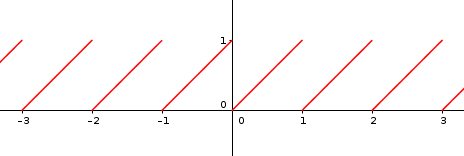
\includegraphics[width=0.5\textwidth]{immagini/esempio_serie_fourier.png}
\end{figure}
\\Osserviamo che nel caso la funzione presa in esame sia pari i coefficienti relativi alla parte dispari dello sviluppo, cioè i $b_n$, saranno tutti nulli, e viceversa, se la funzione è dispari, avremo che gli $a_n$, coefficienti relativi alla parte pari dello sviluppo, saranno tutti nulli.\\
Definiamo ora le somme parziali come la funzione:
$$S_N=a_0 + 2 \sum_{n=1} ^{N} \left[ a_n cos \left( \frac{2 \pi n}{b-a}x \right) + b_n sen \left( \frac{2 \pi n}{b-a}x \right) \right]$$
Quando si verifica che $S_N \to f$? Risostituendo le espressioni dei coefficienti $a_0$, $a_n$, $b_n$ e raccogliendo i fattori comuni, otteniamo otteniamo:
$$S_N=\frac{1}{b-a} \int_a ^b dy f(y) + 2 \sum_{n=1} ^{N} \left[ \frac{1}{b-a} \int_a ^b dy f(y) cos \left( \frac{2 \pi n}{b-a}y \right) cos \left( \frac{2 \pi n}{b-a}x \right) + \right.$$
$$\left. + \frac{1}{b-a} \int_a ^b dy f(y) sen \left( \frac{2 \pi n}{b-a}y \right) sen \left( \frac{2 \pi n}{b-a}x \right) \right]=$$
$$=\frac{1}{b-a} \int_a ^b dy f(y) \left\{ 1 + 2 \sum_{n=1} ^{N} \left[ cos \left( \frac{2 \pi n}{b-a}y \right) cos \left( \frac{2 \pi n}{b-a}x \right) + sen \left( \frac{2 \pi n}{b-a}y \right) sen \left( \frac{2 \pi n}{b-a}x \right) \right] \right\}=$$
$$=\frac{1}{b-a} \int_a ^b dy f(y) \left[ 1 + 2 \sum_{n=1} ^{N}  cos \left( \frac{2 \pi n}{b-a}(x-y) \right)\right] = \int_a ^b dy D_N(x-y) f(y)$$
dove abbiamo definito il \textbf{kernel di Dirichelet} $D_N$ come:
$$D_N=\frac{1}{b-a} \left[ 1 + 2 \sum_{n=1} ^{N}  cos \left( \frac{2 \pi n}{b-a}(x-y) \right)\right]$$
Una particolarità di tale operatore è che soddisfa l'equazione $ \int_a ^b dy D_N(x-y)=1$.
\subsection{Convergenza puntuale}
Se la funzione (sviluppata in serie di Fourier) $f$ è continua a meno di punti di discontinuità di prima specie tali per cui esistano le derivate da destra e da sinistra in tale punto, allora si verifica che $S_N \to f$ dove essa è continua, mentre converge nel ''punto medio'' dove $f$ presenta punti di discontinuità.\\
Se la funzione è molto liscia, allora i coefficienti della serie decresceranno molto rapidamente, altrimenti decrescono lentamente; questo ci porta a concludere c'è una relazione fra i coefficienti della serie di Fourier e le proprietà analitiche della funzione in esame.\\
Un'altra proprietà del kernel di Dirichelet è quella legata alla sua convergenza: infatti, per $N \to \infty$, abbiamo che il kernel $D_N(x-y) \to \delta (x-y)$ ripetuta infinite volte, poichè siamo in presenza di funzioni periodiche.\\
Per dimostrare che i coefficienti tendono ad annullarsi, scriviamo (detto $w=\frac{2 \pi}{b-a}$):
$$\int_a^b dx f(x) sen(wnx)=\int_a^b dx f(x) \left[\frac{d}{dx}\left(-\frac{cos(wnx)}{wn}\right)\right]=$$
$$=-\frac{f(x)cos(wnx)}{wn} + \int_a^b dx f'(x) \frac{cos(wnx)}{wn} \to 0 \text{ per } n \to \infty$$
Notiamo, infatti, che nel caso della funzione $f(x)cos(wnx)$, mediamo sia su valori positivi sia su valori negativi, e quindi quando $n$ è molto grande, abbiamo quasi il profilo della funzione ripetuto sia nella ''zona positiva'' sia nella ''zona negativa'' (sulle y). Per i $b_n$ procediamo in maniera simile.\\
A riguardo dell'annullamento dei coefficienti, risulta importante il seguente risultato dovuto a Riemann e Lebesgue:
\begin{teorema}
Se $f \in \cont^k([a;b])$, allora i coefficienti della serie di Fourier $a_n$, $b_n$ si annullano almeno come $\frac{1}{n^k}$ (per $n \to \infty$).
\end{teorema}
\subsection{Kernel di Fejer}
La teoria delle serie trigonometriche sviluppata da Lipot Fejer ci permette di provare la completezza degli spazi di Banach $\cont([- \pi ; \pi])$, $\L^1([- \pi ; \pi])$ e $\L^2 ([- \pi ; \pi])$. Questo ci assicura che qualsiasi funzione può essere approssimata con una combinazione finita di funzioni trigonometriche. \\
Una funzione $2 \pi$-periodica potrebbe ammettere serie di Fourier non convergente, e quindi non essere riprodotta come limite $N \to \infty$; a questo scopo, definiamo la somma di Fejer come la media aritmetica delle somme parziali, cioè:
$$\sigma _N= \frac{1}{N} \sum_{k=1} ^{N-1} S_k (x)= \int_{-\pi} ^{\pi} dt f(x+t) \Phi _N(t)$$
Dove $\Phi _N(t)$ è il \textbf{kernel di Fejer}, definito come:
$$\Phi _N(t)= \frac{1}{N} \sum_{k=1} ^{N-1} D_k (t)= \frac{1}{2 \pi} + \frac{1}{\pi} \sum_{k=1} ^{N-1} \left(1- \frac{k}{N} \right) cos(kt)= \frac{1}{2 \pi N} \frac{sen^2\left(\frac{Nt}{2}\right)}{sen^2\left(\frac{t}{2}\right)}$$
Tale scrittura ci permette di superare i problemi sopra esplicitati, e di approssimare la funzione come combinazione lineare di funzioni trigonometriche, senza ricorrere alla serie di Fourier.\\
Citiamo ora due teoremi, che non saranno qui dimostrati:
\begin{teorema}(Primo teorema di Fejer)\\
Se $f$ è reale continua e $2 \pi$-periodica, la successione di funzioni $\sigma _N$ converge uniformemente a $f$ in $\R$.
\end{teorema}
\begin{teorema}(Secondo teorema di Fejer)\\
Se $f \in \L^1([-\pi;\pi])$, la successione di somme di Fejer converge af $f$ in $\L^1([-\pi;\pi])$.
\end{teorema}
\section{Funzionali lineari e operatori aggiunti}
\begin{teorema}(Teorema di Riesz)\\
sia $F: \H \to \C$ un funzionale lineare continuo; allora esiste unico $x_F \in \H$ tale che $Fx=(x_F|x)$ $\forall x$ e $\|F\|=\|x_F\|$.
\end{teorema}
\begin{osservazione}
Per dimostrare questo teorema, esplicitiamo una proprietà del $\ker$ di un operatore. Sia $\hat{A} \in \mathcal{B}(\H)$, e sia $\H^*$ come definito in precedenza; allora l'insieme $\ker \hat{A}= \left\{ x: \, \hat{A}x=0 \right\}$ è chiuso. Infatti, presa una successione $x_n \in \ker \hat{A}$, e detto $x$ il limite di tale successione, per la continuità di $\hat{A}$ abbiamo che $\hat{A}x_n \to \hat{A}x$; ma allora, $\hat{A}x=0$, cioè $x \in \ker \hat{A}$.
\end{osservazione}
\begin{proof}
Nel caso banale, abbiamo che il $\ker F = \H$, cioè l'azione di $F$ su qualsiasi elemento $x$ è $Fx=0$; in questo caso, abbiamo che $x_F=0$.\\
Se invece il $\ker F$ non corrisponde con tutto lo spazio di Hilbert, possiamo scomporre $\H$ nella somma diretta di due sottospazi, $\ker F$ e $\ker F ^{\perp}$. Fissiamo ora un $y$ ortogonale all'insieme $\ker F$; per un $x$ generico, scegliamo $\lambda$ tale che $x+\lambda y \in \ker F$, cioè $F(x+\lambda y)=0$; risolvendo tale condizione, troviamo che $\lambda = -\frac{Fx}{Fy}$. La richiesta che $y$ non appartenga al $\ker F$ (è ortogonale ad esso) fa in modo che tale scrittura sia sempre ben posta. Possiamo quindi scrivere:
$$0=(y|x+\lambda y)=(y|x  -\frac{Fx}{Fy} y)=(y|x)  -\frac{Fx}{Fy} \|y\|^2 \implies Fx= \frac{Fy}{\|y\|^2} (y|x)= (x_F|x) \text{, dove } x_F=\frac{F^*y}{\|y\|^2} y$$
Per dimostrarne l'unicità, ipotizziamo che esistano due scritture equivalenti di questo tipo, $(x_F|x)$ e $(\tilde{x}|x)$, e che esse siano coincidenti $\forall x$; allora, abbiamo che:
$$0=(x_F|x) - (\tilde{x}|x)=(x_F - \tilde{x}|x) \, \, \forall x \implies x_F - \tilde{x}=0 \implies x_F = \tilde{x}$$
cioè la scrittura è unica.

Infine, dimostriamo l'identità delle norme:
$$|Fx|=|(x_P|x)| \leq \footnote{Applichiamo la disuguaglianza di Schwarz.} \|x_F\| \, \|x\| \implies \frac{|Fx|}{\|x\|} \leq \|x_F\| \implies \sup_{x, x \neq 0} \frac{|Fx|}{\|x\|} \leq \|x_F\|$$
quindi, preso $x=x_F$, abbiamo che $|Fx_F|=(x_F|x_F)=\|x_F\|^2$; dunque:
$$\frac{|Fx_F|}{\|x_F\|} =\frac{\|x_F\|^2}{\|x\|}= \|x_F\| \text{, cioè  } \|F\|=\|x_F\|$$
che è la tesi.
\end{proof}
Sia ora dato un operatore lineare limitato $\hat{A} \in \mathcal{B}(\H)$, il cui dominio è $\H$; il funzionale $(x|\hat{A} \cdot ): \H \to \C$ è lineare ed è limitato. Dimostriamone la limitatezza utilizzando il lemma di Schwatz:
$$|(x|\hat{A}y)|\leq \|x\| \, \|\hat{A}y\| \leq (\|x\| \, \|\hat{A}\|)\|y\|$$
dove la parentesi è una costante; abbiamo quindi dimostrato la limitatezza.
Possiamo applicare il teorema di Riesz al funzionale; abbiamo che $\forall x \in \H$ esiste un valore $\alpha_x$ tale che $(x|\hat{A}y)=(\alpha_x|y)$ $\forall y \in \H$. Preso un'altro valore $x'$, possiamo applicare lo stesso ragionamento, trovando un valore $\alpha_{x'}$; oltretutto, abbiamo che:
$$(x|\hat{A}y)+(x'|\hat{A}y)=(x+x'|\hat{A}y)=(\alpha_{x+x'}|\hat{A}y)$$
dove l'ultimo passaggio è possibile per il teorema si Riesz; però i primo membro è anche uguale a $(\alpha_x+\alpha_{x'}|\hat{A}y)$, cioè l'associazione $x \mapsto \alpha_x$ è lineare. Chiameremo tale associazione \textbf{operatore aggiunto}, e si indica come $\hat{A}^{\dagger} x= \alpha_x$.
\begin{teorema}
Sia $\hat{A} \in \mathcal{B}(\H)$; allora esiste $\hat{A}^{\dagger} \in \mathcal{B}(\H)$ tale che:
$$(x|\hat{A}y)=(\hat{A}^{\dagger}x|y)$$
$$\|\hat{A}\|=\|\hat{A}^{\dagger}\|$$
\end{teorema}
\begin{proof}
La linearità l'abbiamo dimostrata in precedenza; ci manca da dimostrarne la limitatezza:
$$\| \hat{A}^{\dagger} x \|^2=(\hat{A}^{\dagger}x|\hat{A}^{\dagger}x)=(x|\hat{A} \hat{A}^{\dagger} x) \leq  \|x\| \, \|\hat{A} \hat{A}^{\dagger} x \| \leq \|x\| \, \|\hat{A}\| \, \|\hat{A}^{\dagger} x \|$$
negli ultimi due passaggi sono stati sfruttati in ordine il lemma di Schwarz e la limitatezza di $\hat{A}^{\dagger}$;  allora abbiamo che:
$$\| \hat{A}^{\dagger} x \| \leq \|\hat{A}\| \, \|x \| \text{ } \forall x$$
e quindi $\hat{A}^{\dagger}$ è limitato, cioè $\hat{A}^{\dagger} \in \mathcal{B}(\H)$; oltretutto, abbiamo che $\|\hat{A}^{\dagger}\| \leq \|\hat{A}\|$.\\
Allo stesso modo, possiamo scrivere:
$$\| \hat{A}y \|^2=(\hat{A}y|\hat{A}y)=(\hat{A}^{\dagger} \hat{A} y|y) \leq  \|y\| \, \|\hat{A}^{\dagger} \hat{A} y \| \leq \|y\| \, \|\hat{A^{\dagger}}\| \, \|\hat{A} y \| \implies \|\hat{A}\| \leq \|\hat{A}^{\dagger}\|$$
Confrontando questo e il risultato precedente, otteniamo:
$$\|\hat{A}^{\dagger}\| \leq \|\hat{A}\| \leq \|\hat{A}^{\dagger}\| \implies \|\hat{A}\| = \|\hat{A}^{\dagger}\|$$
che è la nostra tesi.
\end{proof}
\clearpage
Lo spazio $\mathcal{B}(\H)$ è chiuso rispetto all'operazione $\dagger: \hat{A} \mapsto \hat{A}^{\dagger}$; le proprietà di tale operazione sono:
\begin{itemize}
\item $(\hat{A}^{\dagger})^{\dagger}= \hat{A}$
\item $( \lambda \hat{A})^{\dagger}= \overline{\lambda} \hat{A}^{\dagger}$
\item $(\hat{A} + \hat{B})^{\dagger}=\hat{A}^{\dagger} + \hat{B}^{\dagger}$
\item $(\hat{A} \hat{B})^{\dagger}=\hat{B}^{\dagger} \hat{A}^{\dagger}$
\end{itemize}
Sia dato un'operatore $\hat{A}$; esso è invertibile se è iniettivo, cioè se , qualora si abbia $\hat{A}x=\hat{A}x'$, allora $x=x'$. La linearità infatti implica che il $\ker$ dell'operatore si riduce al solo $0$; infatti, se risolviamo $\hat{A}(x-x')=0$, otteniamo che per iniettività si deve avere $x-x'=0$.\\
Cerchiamo ora una relazione fra un operatore e il suo aggiunto:
$$(Im \hat{A})^{\perp} = \left\{x \in \H : \, (x|\hat{A}y)=0 \, \forall y \in \H \right\} = \left\{x \in \H : \, (\hat{A} ^{\dagger}x|y)=0 \, \forall y \in \H \right\}=$$
$$=\left\{x \in \H : \hat{A}^{\dagger} x=0 \right\}= \ker \hat{A}^{\dagger}$$
Quindi $\ker \hat{A}^{\dagger}$ è un'insieme chiuso perchè è uguale a $(Im \hat{A})^{\perp}$, che è un'insieme chiuso. Possiamo quindi scrivere:
$$\H= \ker \hat{A} \oplus (\ker \hat{A})^{\perp}=(Im \hat{A})^{\perp} + \overline{Im \hat{A}^{\dagger}}$$
E, dato che l'uguaglianza vale termine a termine, possiamo sommare un termine di $\ker$ e un termine di $Im$ (non a caso); questo è importante quando dobbiamo risolvere un'equazione del tipo $\hat{A}x=y$: infatti, se siamo in uno spazio finito-dimensionale, abbiamo delle condizioni che devono essere soddisfatte per poter discutere la risolubilità (ad esempio, l'invertibilità della matrice). Se invece siamo in uno spazio $\infty$-dimensionale, ci chiediamo se $y \in Im \hat{A}$.\footnote{Alternativamente, possiamo utilizzare il metodo di Fredom, secondo il quale se $\ker \hat{A}^{\dagger}=0$ allora esiste una soluzione.}
\begin{definizione}
Un'operatore $\hat{A} \in \mathcal{B}(\H)$ si dice \textbf{autoaggiunto} se $\hat{A}=\hat{A}^{\dagger}$, cioè se vale che:
$$(\hat{A}x|y)=(x|\hat{A}^{\dagger}y) \, \, \forall x, y \in \H$$
\end{definizione}
Un esempio di operatore autoaggiunto che abbiamo già visto in precedenza è il proiettore ortogonale; infatti avevamo visto che fra le proprietà di tale operatore c'era proprio l'essere autoaggiunto; inoltre, detto $Im \hat{P}$ sottospazio di proiezione, abbiamo che nel caso in cui tale sottospazio abbia dimensione finita, vale che $\tr \hat{P}=\dim Im \hat{P}$.
\begin{definizione}
Lo scalare $\lambda \in \C$ si dice \textbf{autovalore proprio} dell'operatore $\hat{A}$ se esiste un elemento $u \in \H$ tale che $\hat{A} u = \lambda u$. Nel caso in cui $\hat{A}$ sia autoaggiunto, allora $\lambda$ è reale.\\
L'insieme degli  autovalori di un operatore è detto \textbf{spettro puntuale} dell'operatore e si indica con $\sigma_P (\hat{A})$.
\end{definizione}
Siano $\lambda , \mu \in \sigma_P (\hat{A})$, cioè siano essi due autovalori dell'operatore $\hat{A}$; se $\lambda \neq \mu$, allora si ha che $(u|v)=0$, dove $u$ e $v$ sono gli autovalori relativi rispettivamente a $\lambda$ e $\mu$. Questo ci dive che possiamo scomporre uno spazio di Hilbert come somma ortogonale  dello spazio generato dagli autovettori (che, come appena visto, sono ortogonali fra loro) e il suo spazio ortogale:
$$\H=\H_P \oplus \H_P ^{\perp}=\H_P \oplus \H_C$$
Nel caso dei proiettori, abbiamo $\H_C=\varnothing$.
\section{Operatori unitari}
Definiamo l'operatore unitario $\hat{U}$ come quell'operatore tale che sia una biezione e che rispetti l'uguaglianza fra norme:
$$\|\hat{U}x\|=\|x\| \, \, \forall x$$
Altre proprietà degli operatori unitari sono:
\begin{itemize}
\item Il prodotto di operatori unitari è unitario.
\item $\ker \hat{U}= \{0\}$
\item Vale che $(\hat{U}x|\hat{U}y)=(x|y)$; da questa proprietà ricaviamo che un'operatore unitario e il suo aggiunto commutano; infatti, per la definizione di aggiunto possiamo scrivere:
$$(\hat{U}x|\hat{U}y)=(\hat{U}^{\dagger} \hat{U} x|y)$$
e, sottraendo il secondo membro dell'equazione di partenza, otteniamo:
$$([\hat{U}^{\dagger} \hat{U} - \mathbb{I}]x|y)=0 \implies \hat{U}^{\dagger} \hat{U} = \mathbb{I}$$
e alla stessa maniera ricaviamo $ \hat{U} \hat{U}^{\dagger} = \mathbb{I}$; mettendo insieme le due condizioni (che valgono $\forall x,y$), si ottiene che il commutatore fra l'operatore e il suo aggiunto è nullo, cioè commutano.
\item Gli autovalori stanno tutti sulla circonferenza unitaria; infatti, detto $\lambda$ autovalore relativo all'autovettore $x$, per l'identità delle norme abbiamo:
$$\|x\|=\|\hat{U}x\|=\|\lambda x\|=|\lambda| \, \|x\| \implies |\lambda|=1$$
\end{itemize}
Abbiamo visto che, dato un operatore $\hat{A} \in \mathcal{B}(\H)$, possiamo sempre ricavarne l'esponenziale $e^{z \hat{A}}$, con $z \in \C$ che è a sua volta un'operatore limitato. Sviluppando in serie, possiamo definire la funzione $S_N(z)$, cioè le somme parziali dello sviluppo in serie nella variabile $z$. saranno della forma:
$$S_N(z)= \sum_{k=0} ^N \frac{(z \hat{A})^k}{k!} \to e^{z \hat{A}} \text{ per } N \to \infty$$
A questo punto, possiamo dimostrare che per gli operatori vale che $e^{(z_1+z_2) \hat{A}}=e^{z_1 \hat{A}} e^{z_2 \hat{A}}$ utilizzando le somme parziali; scriviamo:
$$S_N(z_1+z_2)=\sum_{k=0} ^N \frac{[(z_1+z_2) \hat{A}]^k}{k!} = \footnote{Sfruttiamo lo sviluppo tramite binomio di Newton.} \sum_{k=0} ^N \frac{ \hat{A}^k}{k!} \sum_{j=0} ^N \frac{k!}{j! (k-j)!} z_1^j z_2 ^{k-j}=$$
$$=\sum_{j=0} ^N \frac{z_1^j}{j!} \sum_{k=j} ^N \frac{z_2 ^{k-j}}{(k-j)!} \hat{A}^k =\sum_{j=0} ^N \frac{z_1^j}{j!} \sum_{k=0} ^{N-j} \frac{z_2 ^k}{k!} \hat{A}^{k+j}= \sum_{j=0} ^N \frac{(z_1 \hat{A})^j}{j!} \sum_{k=0} ^{N-j} \frac{(z_2 \hat{A})^k}{k!} = S_N(z_1) S_N(z_2)$$
e, nel limite di $N \to \infty$, abbiamo la tesi.\\
Nel caso in cui $\hat{A}$ sia autoaggiunto, possiamo definire l'esponenziale $e^{it\hat{A}}$, con $t \in \R$; tale operatore esponenziale è un'operatore unitario, e quindi commuta con il suo aggiunto. Infatti, detto $\hat{U}$ l'operatore esponenziale, si ha:
$$\hat{U}^{\dagger} (t)= \left(e^{it\hat{A}}\right)^{\dagger}=e^{-it\hat{A}^{\dagger}}=\hat{U}(-t)$$
e dunque, il prodotto $\hat{U}^{\dagger} \hat{U}$ dà l'identità, e la stessa cosa scambiando i fattori. L'operatore $i \hat{A}$ (dove $\hat{A}$ e come definito in precedenza) è detto \textbf{operatore antiautoaggiunto}, poichè il suo aggiunto è il suo opposto, cioè è autoaggiunto a meno di un segno.\\
L'insieme di operatori $\hat{U} (t)$ è un gruppo a un parametro (che è $t$) di operatori unitari, con continuità forte nell'origine, cioè:
$$\lim_{t \to 0} \| \hat{U}(t) x - x \|_{\H}=0$$
La matrice che genera tale gruppo di operatori è detta \textbf{generatore del gruppo a un parametro}.
\begin{teorema}
Sia $\hat{U} (t)$ un gruppo a un parametro di operatori unitari fortemente continuo. Allora esiste un'operatore autoaggiunto $\hat{H}$, in generale non limitato, tale che:
$$\hat{U}(t)=e^{-it \hat{H}}$$
Si ha inoltre che il dominio di tale operatore è:
$$\mathcal{D} (\hat{H})= \left\{x \in \H \text{ : } \exists \lim_{t \to 0} \frac{e^{-it\hat{H}} x - x}{-it} \right\}$$
\end{teorema}
Sia dato l'operatore $\hat{A}$ a valori in $\H$; abbiamo definito l'operatore aggiunto $\hat{A}^{\dagger}$ come quell'operatore tale per cui $(x|\hat{A}y)=(\hat{A}^{\dagger} x|y)$ $\forall x \in \mathcal{D}({\hat{A}^{\dagger}})$, $\forall y \in \mathcal{D}({\hat{A}})$. In quale occasione possiamo trovare l'operatore aggiunto? Solo nel caso in cui il dominio di tale operatore sia della forma:
$$\mathcal{D}({\hat{A}^{\dagger}})=\left\{ x \in \H \text{ : } \forall y \in \mathcal{D}({\hat{A}}) \, \exists ! \tilde{x} \text{ : } (x|\hat{A}y)=(\tilde{x}|y) \right\}$$
Una volta caratterizzata in questa maniera il dominio, diremo che $\tilde{x}=\hat{A}^{\dagger} x$.\\
Ragioniamo sulla richiesta di unicità: supponiamo che, fissato $x$, esistano $\tilde{x}$ e $x'$ tali che $(\tilde{x}|y)=(x|\hat{A}y)$ e $(x'|y)=(x|\hat{A}y)$ $\forall y \in \mathcal{D}(\hat{A})$; sottraendo membro a membro le due uguaglianze, otteniamo:
$$(\tilde{x} - x'|y)=0 \, \, \forall y \in \mathcal{D}(\hat{A})$$
cioè $(\tilde{x}-x') \in (\mathcal{D}(\hat{A}))^{\perp}$. La richiesta di unicità ci permette di concludere che $\tilde{x}=x'$, cioè che $(\mathcal{D}(\hat{A}))^{\perp} = \left\{0\right\}$, cioè che $\overline{\mathcal{D}(\hat{A})}= \H$. Quindi l'operatore deve essere \textbf{densamente definito}, cioè per ogni elemento dello spazio di Hilbert è limite di una successione di elementi di $\hat{A}$.\\
Adesso dimostriamo che, dato $\hat{A} \in \mathcal{B}(\H)$,  vale la relazione $\| \hat{A}^{\dagger} \hat{A} \|= \| \hat{A} \|^2$; utilizzando la proprietà della norma tale per cui $\| \hat{A} \hat{B} \| \leq \| \hat{A} \| \, \| \hat{B} \|$, scriviamo:
$$\| \hat{A}^{\dagger} \hat{A} \| \leq \|\hat{A}^{\dagger}\| \, \|\hat{A}\|= \|\hat{A}\| \, \|\hat{A}\| = \|\hat{A}\|^2$$
Inoltre, sfruttando la disuguaglianza di Schwarz, possiamo scrivere:
$$\| \hat{A}x\|^2=(\hat{A}x|\hat{A}x)=(\hat{A}^{\dagger} \hat{A}x|x) \leq \| \hat{A}^{\dagger} \hat{A}\| \, \|x\|$$
e, prendendo il sup, otteniamo:
$$\|\hat{A}\| = \sup_{x \neq 0} \frac{\|\hat{A}x\|}{\|x\|} \leq \|\hat{A}^{\dagger} \hat{A}\|^{\frac{1}{2}}$$
unendo le due condizioni, dimostriamo la tesi.\\
Possiamo definire la norma di un'operatore in altro modo:
$$\|\hat{A}\|=\sup_{\|x\|=1} |(x|\hat{A}x)|$$
\clearpage
\section{Spazi di Schwarz}
A Schwarz si deve l'introduzione di due spazi: lo \textbf{spazio di Schwarz}, cioè lo spazio delle funzioni $\cont^{\infty}$ a decrescenza rapida, indicato nella forma $\S(\R)$, e lo spazio $\mathscr{D}(\R)$, cioè lo spazio delle funzioni $\cont^{\infty}$ a supporto compatto; notiamo che lo spazio $\mathscr{D}$ è contenuto nello spazio $\S$.\\
Inoltre, a partire da questi due spazi, possiamo definirne altri due: lo spazio delle \textbf{distribuzioni temperate} $\S'(\R)$ e lo spazio delle distribuzioni $\mathscr{D}'(\R)$; in questo caso, invece, abbiamo che lo spazio $\S'$ è contenuto nello spazio $\mathscr{D}'$.\\
Una proprietà fondamentale dello spazio di Schwarz $\S$ è quella di essere invariante per la trasformata di Forier, cioè tale operatore, che definiremo poco più avanti, manda $\S$ in se stesso; inoltre, lo spazio $\S$ è sottoinsieme dello spazio $\L^2$ e la sua chiusura (nella norma di $\L^2$) è proprio lo spazio $\L^2$.\\
Il contributo di Gelfrand è molto importante nello studio di questi spazi; infatti egli introdusse le cosìddette \textbf{funzioni generalizzate} (come ad esempio la delta di Dirach), che permettono di trattare distribuzioni con strumenti pensati per le funzioni.
\\
\\
Prima però di passare allo studio delle distribuzioni, trattiamo più approfonditamente  i concetti appena introdotti; prima di tutto, diamo una definizone di \textbf{decrescenza rapida}:
\begin{definizione}
Una funzione $f$ si dice a \textbf{decrescenza rapida} se, $\forall m,n \geq 0$, esiste finita la quantità:
$$\|f\|_{m,n} = \sup_{x \in \R} |x^m (D^n f)(x)|$$
dove abbiamo indicato con $D^n$ l'operazione di derivata $n$-esima, cioè $D^n=\frac{d^n}{dx^n}$.
\end{definizione}
La decrescenza rapida mi permette quindi di fare in modo che tale quantità non esploda ad infinito qualsiasi valore io scelga per le costanti $n$ e $m$. Funzioni di questo tipo sono per esempio $e^{-x^2}$ e i polinomi di Hermite. Notiamo che l'operazione $\| \cdot \|_{m,n}$ definisce una \textbf{famiglia di seminorme}, poichè rispetta le seguenti proprietà:
\begin{itemize}
\item $\| \phi_1 + \phi_2 \|_{m,n} \leq \| \phi_1\|_{m,n} + \|\phi_2\|_{m,n}$
\item $\| \lambda \phi \|_{m,n} = | \lambda | \, \| \phi \|_{m,n}$
\end{itemize}
Lo spazio $\cont(\R)$ è lo spazio delle funzioni continue che si annullano ad $\infty$; esso è uno spazio di Banach, dove la norma è definita come:
$$\|f\|= \sup_x |f(x)|$$
Si verifica che $\S \subset \cont$. Un'altra inclusione importante per lo studio dello spazio di Schwarz è $\S \subset \L^1$; detto ciò, presa una funzione $\phi \in \S$, abbiamo che:
$$\| \phi \|_1 = \int_{- \infty} ^{+\infty} dx | \phi (x) |= \int_{- \infty} ^{+\infty} dx | \phi (x) | \frac{1+x^2}{1+x^2} \leq \sup_x | \phi (x) (1+x^2)| \int_{- \infty} ^{+\infty} dx \frac{1}{1+x^2}=$$
$$=\sup_x | \phi (x) (1+x^2)| \pi  \leq \left( \| \phi \|_{0,0} + \| \phi \|_{2,0} \right) \pi$$
Allo stesso modo, possiamo dimostrare che $\S \subset \L^p$:
$$\| \phi \|_p ^p = \int_{- \infty} ^{+\infty} dx | \phi (x) |^p = \int_{- \infty} ^{+\infty} dx | \phi (x) |^{p-1} | \phi (x) | \leq \| \phi \|_{0,0} \int_{- \infty} ^{+\infty} dx | \phi (x) |^{p-1} \leq \dots \leq \| \phi \|_{0,0} ^{p-1} \, \| \phi \|_1$$
Definiamo ora la convergenza in $\S(\R)$:
\begin{definizione}
Una successione $\phi_r$ converge a $\phi$ in $\S$ se $\| \phi_r - \phi \|_{m,n} \to 0$ $\forall m,n$.
\end{definizione}
\clearpage
Per far sì che lo spazio sia completo, ci rimane da introdurre la nozione di successione di Cauchy:
\begin{definizione}
Una successione è di Cauchy se
$$\forall \epsilon >0 \, \, \exists N_{\epsilon , m,n} \text{ : }\|\phi_r -\phi_s \|_{m,n} < \epsilon \, \, \forall r,s > N_{\epsilon , m,n} \text{, con }m,n=0,1 \dots$$
\end{definizione}
Ora quindi possiamo enunciare il seguente teorema:
\begin{teorema}
Lo spazio $\S(\R)$ è completo.
\end{teorema}
Quando sono completi, questi spazi non sono più detti spazi di Banach, ma \textbf{spazi di Frechet}.
Nella definizione di successione di Cauchy, riscriviamo la norma come da definizione, cioè $\| \phi_r - \phi_s \| = \sup_{x \in \R} |x^m D^n (\phi_r - \phi_s)|$. Notiamo che, nel caso in cui $m=n=0$, allora la convergenza in $\S$ coincide con la convergenza per funzioni reali a variabili reali; quindi  $\phi_r$ è una successione di Cauchy in $\cont(\R)$, cioè converge alla funzione $\psi_{0,0} \in \cont(\R)$. Generalizzando per ogni coppia di $m,n$, abbiamo che $x^m D^n \phi_r$ è una successione di Cauchy nello spazio $\cont(\R)$, cioè converge alla funzione $\psi_{m,n} \in \cont(\R)$; si dimostra che $\psi_{m,n}=x^m D^n \psi_{0,0}$.
\\
Passiamo ora a trattare gli operatori sullo spazio $\S$:
\begin{itemize}
\item \textbf{Operatore di moltiplicazione $\hat{Q}$}: tale operatore è definito in $\S$ a valori in $\S$ ed è continuo; la sua azione sulla funzione $\phi \in \S$ è:
$$(\hat{Q} \phi)(x)=x \phi(x)$$
Dimostriamo che la norma in $\S$ di tale operatore è finita, cioè che $\hat{H}\phi \in \S$:
$$\sup_x |x^m D^n (\hat{Q} \phi)(x)|=\sup_x |x^m D^n (x \phi)|= \sup_x |x^m D^{n-1} \phi + x^{m+1} D^n \phi| \leq$$
$$\leq \sup_x |x^m D^{n-1} \phi| + \sup_x |x^{m+1} D^n \phi|= \| \phi \|_{m,n-1} + \| \phi \|_{m+1,n}$$
Quindi, poichè le due seminorme sono quantità finte, abbiamo che anche la seminorma dell'operatore è finita e dunque $\hat{Q} \phi \in \S$. Dimostriamo ora la continuità dell'operatore; data la linearità di $\hat{Q}$, ci basta dimostrarne la continuità nell'origine. Data una successione $\phi_r$ che converge a $0$ in $\S$ per $r \to \infty$, abbiamo che $\hat{Q} \phi_r \to 0$ in $\S$; infatti, passando alle seminorme, abbiamo che la seminorma $\| \hat{Q} \phi \|_{m,n}$ è minorata dalla somma di due seminorme della funzione $\phi_r$ e, dato che la condizione di annullamento di $\phi_r$ equivale a dire che $\| \phi_r \|_{m,n} \to 0$ $\forall m,n$, abbiamo che le due seminorme tendono ad annullarsi nel limite per $r \to \infty$, e dunque anche l'operatore applicato a $\phi_r$ tende a $0$.
\item \textbf{Operatore $\hat{P}$}: anch'esso definito in $\S$ a valori in $\S$ e continuo, ha azione descritta da:
$$\hat{P} \phi = -i D \phi$$
dove ricordiamo che la $D$ indica l'operazione di derivazione; l'operatore risulta invertibile, poichè si ha che $\ker \hat{P} = \left\{ 0 \right\}$: infatti la derivata di $\phi$ si annulla solo nel caso in cui $\phi$ sia costante e, dato che siamo nello spazio $\S$, non può che essere $\phi = 0$.
\end{itemize}
\section{La trasformata di Fourier}
Definiamo su $\S$ due operatori lineari:
$$\left( \F \phi \right) (k) = \int_{-\infty} ^{+\infty} \frac{dx}{\sqrt{2 \pi}} e^{-ikx} \phi (x)$$
$$\left( \F^{-1} \phi \right) (k) = \int_{-\infty} ^{+\infty} \frac{dx}{\sqrt{2 \pi}} e^{ikx} \phi (x)=\left( \F \phi \right) (-k)$$
dove $k$ è un parametro definito in $\R$.

La prima è detta \textbf{trasformata di Fourier}, la seconda \textbf{antitrasformata di Fourier}. Osserviamo che entrambe sono definite in $\S$ a valori in $\S$ e $\F \phi \in \cont^{\infty}$ (possiamo portare la derivata all'interno dell'integrale e otteniamo che $x^n \phi \in \S$); verifichiamo quindi che $\| \F \phi \|_{m,n} < \infty$ $\forall m,n$:
$$x^m D_x ^n \left( \F \phi \right) (x) = x^m \int_{-\infty} ^{+\infty} \frac{dk}{\sqrt{2 \pi}} \left( D_x ^n e^{-ikx} \right) \phi (k) = x^m \int_{-\infty} ^{+\infty} \frac{dk}{\sqrt{2 \pi}} (-ik)^n e^{-ikx} \phi (k) =\footnote{Possiamo portare dentro l'integrale $x^m$, poichè stiamo integrando su $k$, e lo vediamo come derivata $m$-esima (rispetto a $k$) dell'esponenziale.}$$
$$= \int_{-\infty} ^{+\infty} \frac{dk}{\sqrt{2 \pi}} \frac{(-ik)^n}{(-i)^m} \left( D^m _k e^{-ikx} \right) \phi (k) =\footnote{Integramo per parti $m$-volte; possiamo ignorare i termini di bordo, poichè la funzione $\phi$ è a decrescenza rapida, e quindi batte qualsiasi potenza.} (-1)^m (-i)^{n-m} \int_{-\infty} ^{+\infty} \frac{dk}{\sqrt{2 \pi}} e^{-ikx} D_k ^m \left( k^n \phi (k) \right)$$
L'operazione di derivazione ci darà al più $m+1$ termini del tipo $x^{\alpha} D^{\beta} \phi$, con $\alpha = n,n-1, \dots ,n-m$ e $\beta=0,1, \dots ,m$; quindi possiamo scrivere:
$$\left|x^m \left(D^n \F \phi \right) (x) \right| \leq \sum_{\alpha, \beta} \int_{-\infty} ^{+\infty} \frac{dk}{\sqrt{2 \pi}} | k^{\alpha} \phi^{\beta} (k) | \frac{1+k^2}{1+k^2} = \pi \Sigma_N [\phi]$$
dove il termine $ \Sigma_N [\phi]$ indica una somma finita di seminorme di $\phi$; quindi abbiamo che la quantità $\| \F \phi \|_{m,n}$ è finita per ogni coppia di valori $m,n$.
\\
\\
Abbiamo detto che la trasformata di fourier è un'operatore lineare che manda $\S$ in $\S$; si ha inoltre che $\F$ è un'operatore continuo, cioè se applicato ad una successione convergente restituisce una successione convergente. Anche in questo caso come per l'operatore di moltiplicazione ci basta  dimostrare la continuità nell'origine, cioè dimostrare la seguente implicazione in $\S$:
$$\phi_r \to 0 \implies \| \F \phi_r \| \to 0$$
Tutte le proprietà enunciate per la trasformata di Fourier valgono anche per l'antitrasformata; adesso, mostriamo che effettivamente i due operatori, come suggerisce la scrittura, sono uno l'inverso dell'altro:
\begin{teorema}(Teorema di inversione per la trasformata di Fourier)\\
L'inverso della trasformata di Fourier $\F$ è l'antitrasformata $\F^{-1}$, cioè $\F \o \F^{-1}= \F^{-1} \o \F= \mathbb{I}$; in forma integrale:
$$ \int_{-\infty} ^{+\infty} \frac{dk}{\sqrt{2 \pi}} e^{-ikx}\left( \F \phi \right) (k) =  \int_{-\infty} ^{+\infty} \frac{dk}{\sqrt{2 \pi}} e^{ikx} \left( \F^{-1} \phi \right) (k) = \phi(x)$$
\end{teorema}
Per dimostrare il teorema, introduciamo prima un lemma che ci sarà molto utile:
\begin{lemma}
sia definito l'operatore $\hat{E_{\epsilon}} (x)= e^{- \epsilon x^2}$; allora abbiamo che $\hat{E_{\epsilon}} \phi \in \S$ e il suo limite in $\S$ per $\epsilon \to 0^+$ è $\phi$.
\end{lemma}
\begin{proof}
Dobbiamo dimostrare che la norma della funzione è finita, cioè che $\sup_x |x^m D^n (e^{- \epsilon x^2} \phi (x))| < \infty$ $\forall m,n$; equivalentemente, possiamo dimostrare che $\sup_x |x^m D^n (e^{- \epsilon x^2} \phi (x)- \phi(x))| \to 0$ per $\epsilon \to 0$ $\forall m,n$.
$$\lim_{\epsilon \to 0} \| \hat{E_{\epsilon}} \phi - \phi \|_{m,n}= \lim_{\epsilon \to 0} \sup_x \left[ (1-e^{- \epsilon x^2})|x^m D^n  \phi (x)|\right]$$
dove possiamo maggiorare il coefficiente $(1-e^{- \epsilon x^2})$ nella seguente maniera:
$$1-e^{- \epsilon x^2} \left\{\begin{matrix} =0 & x=0 \\ \leq 2 \epsilon x^2 & x \neq 0 \end{matrix} \right.$$
e quindi nel limite di $\epsilon \to 0$ la norma si annulla sempre.
\end{proof}
Dunque, se $\hat{E_{\epsilon}} \phi$ tende a $0$ nel limite per $\epsilon \to 0$, allora, per la continuità della trasformata e dell'antitrasformata, abbiamo che $\F^{-1} \left(\hat{E_{\epsilon}}\left(\F \phi \right) \right) \to \F^{-1} \F \phi$ in $\S$; possiamo utilizzare questa proprietà per dimostrare che $\F^{-1} \F \phi = \phi$ o, equivalentemente, che $\F^{-1} \F \phi - \phi = 0$.\\
Abbiamo che:
$$\F ^{-1} \hat{E_{\epsilon}} \F \phi = \int_{-\infty} ^{+\infty} \frac{dk}{\sqrt{2 \pi}} e^{ikx} e^{-\epsilon k^2} \int_{-\infty} ^{+\infty} \frac{dy}{\sqrt{2 \pi}} e^{-iky} \phi (y)$$
Cambiando ordine di integrazione, otteniamo:
$$\int_{-\infty} ^{+\infty} dy \phi (y) \int_{-\infty} ^{+\infty} \frac{dk}{2 \pi} e^{-ik(y-x) -\epsilon k^2} = \int_{-\infty} ^{+\infty} dy \phi (y) \int_{-\infty} ^{+\infty} \frac{dk}{2 \pi} e^{- \epsilon \left( k + \frac{y-x}{2 \epsilon} \right)^2  -\frac{(y-x)^2}{4 \epsilon}} =$$
$$= \int_{-\infty} ^{+\infty} dy \phi (y) e^{ -\frac{(y-x)^2}{4 \epsilon}} \frac{1}{2 \pi} \frac{\sqrt{\pi}}{\sqrt{\epsilon}} =  \int_{-\infty} ^{+\infty} dy \phi (y) k_{\epsilon} (x-y)$$
Dove abbiamo abbiamo definito il kernel dell'equazione del calore:
$$ k_{\epsilon} (x-y) = \frac{1}{2 \sqrt{ \pi \epsilon}} e^{ -\frac{(y-x)^2}{4 \epsilon}}$$
Notiamo che, per $\epsilon \to 0$, tale kernel tende alla $\delta (x-y)$; inoltre, abbiamo che il kernel è normalizzato, cioè $ \int_{-\infty} ^{+\infty} dx k_{\epsilon} (x)=1$. Ora, ci rimane da dimostrare che:
$$\lim_{\epsilon \to 0}  \int_{-\infty} ^{+\infty} dy \left( \phi (y) - \phi (x) \right) k_{\epsilon} (x-y)=0$$
Per farlo, prendiamo il modulo e maggioriamo:
$$|\int_{-\infty} ^{+\infty} dy \left( \phi (y) - \phi (x) \right) k_{\epsilon} (x-y)| \leq \int_{-\infty} ^{+\infty} dy | \phi (y) - \phi (x) | \, |k_{\epsilon} (x-y)| \leq$$
$$ \leq \int_{-\infty} ^{+\infty} dy |\phi' (\xi_{x,y})| \, |x-y| \frac{1}{2 \sqrt{ \pi \epsilon}} e^{ -\frac{(y-x)^2}{4 \epsilon}} \leq \footnote{Eseguiamo un cambio di variabili $z=x-y$.} \sup_z |\phi' (\xi_{x,y})| \int_{-\infty} ^{+\infty} dz |z|  \frac{1}{2 \sqrt{ \pi \epsilon}} e^{ -\frac{(y-x)^2}{4 \epsilon}}$$
Dunque, abbiamo che:
$$|\F^{-1} \hat{E_{\epsilon}} \F \phi - \phi| \leq 2 \| \phi \|_{0,1} \int_0 ^{+\infty} dz \frac{z}{2 \sqrt{ \pi \epsilon}} e^{ -\frac{(y-x)^2}{4 \epsilon}}= \footnote{Altro cambio di variabili; in questo caso, scriviamo $z= \sqrt{\epsilon} t$.} 2 \| \phi \|_{0,1}  \frac{\sqrt{\epsilon}}{2 \sqrt{\pi}} \int_0 ^{+\infty} dt \, t \,  e^{ -\frac{t^2}{4}}$$
che, nel limite per $\epsilon \to 0$, tende a 0.
\subsection{Proprietà della trasformata di Fourier}
Abbiamo introdotto la trasformata $\F$ e l'antitrasformata $\F^{-1}$ come operatori definiti in $\S$ a valori in $\S$; oltretutto, tramite il teorema di inversione, abbiamo visto che $\F \o \F^{-1}=\mathbb{I}$. Altre proprietà utili di quest'operatore sono:
\begin{itemize}
\item L'operatore $\F$ elevato al quadrato si comporta come l'operatore parità, cioè si ha che $(\F^2 \phi )(x)=\phi(-x)$; infatti, per dimostrarlo basta dire che $(\F^2 \phi )(x)=(\F^{-1} \F \phi)(-x)= (\mathbb{I} \phi)(-x)= \phi(-x)$
\item Valgono le seguenti identità fra operatori:
$$\F \hat{Q}=-\hat{P}\F$$
$$\hat{Q} \F= \F \hat{P}$$
Dimostriamo la seconda; la prima si dimostra in modo analogo. Vale che:
$$(\hat{Q} \F \phi)(x)=x(\F \phi)(x) = x \int_{-\infty}^{+\infty} \frac{dk}{\sqrt{2 \pi}}e^{-ikx} \phi(k)=  \int_{-\infty}^{+\infty} \frac{dk}{\sqrt{2 \pi}} i \left( \frac{d}{dk} e^{-ikx} \right) \phi(k)$$
a questo punto, integriamo per parti; i termini di bordo si annullano, e ci rimane:
$$(\hat{Q} \F \phi)(x)=-i \int_{-\infty}^{+\infty} \frac{dk}{\sqrt{2 \pi}}e^{-ikx} \phi'(k)=(\F (-i \phi'))(x)=(\F \hat{P} \phi)(x)$$
\item $\left[ \hat{Q}^2 + \hat{P}^2 , \F \right]=0$
\item $(\F u_n)(x)= (-i)^n u_n (x)$, cioè la trasformata di Fourier di una funzione di Hermite è una funzione di Hermite; dunque le funzioni di Hermite sono autovettori della trasformata di Fourier relativi agli autovalori $(-i)^n$. %Per dimostrare questo fatto, si trova la funzione generatrice degli $u_n$, che sarà nella forma:
%$$h(t,x)=\sum_{n=0}^{\infty} \frac{t^n}{\sqrt{n!}} \frac{1}{\sqrt{n! 2^n \sqrt{\pi}}} e^{\frac{x^2}{2}} H_n(x)$$
%notiamo che 
\item $(\phi|\F \psi)=(\F^{-1} \phi|\phi)$; se sosituiamo la $\phi$ con $\F \xi$, otteniamo che:
$$(\F \xi | \F \psi )=(\xi|\psi) \text{ } \forall \phi, \psi, \xi \in \S(\R)$$
cioè abbiamo che la trasformata di Fourier si comporta come un operatore unitario. Dimostriamo questa proprietà:
$$(\phi | \F \psi)= \int_{-\infty} ^{+\infty} dx \overline{\phi (x)} \left(\F \psi \right) (x)= \int_{-\infty} ^{+\infty} dx \overline{\phi (x)}  \int_{-\infty} ^{+\infty} \frac{dk}{\sqrt{2 \pi}} e^{-ikx} \psi(k)=$$
$$=\int_{-\infty} ^{+\infty} \frac{dk}{\sqrt{2 \pi}} \left[ \int_{-\infty} ^{+\infty} dx \overline{\phi (x)} \, \overline{e^{ikx}}  \right] \psi(k) =  \int_{-\infty} ^{+\infty} dk \overline{\left( \F^{-1} \phi \right) (k)} \psi(k)=(\F^{-1} \phi | \psi)$$
Inoltre, grazie al teorema dell'inversione, possiamo scrivere:
$$\phi(x)=\left(\F^{-1} \F \phi \right) (x) = \int_{-\infty} ^{+\infty} dk \frac{e^{ikx}}{\sqrt{2 \pi}} \left(\F \phi \right) (x) =  \int_{-\infty} ^{+\infty} dk \frac{e^{ikx}}{\sqrt{2 \pi}} \tilde{\phi} (k)$$
dove abbiamo che $\tilde{\phi} (k)=  \int_{-\infty} ^{+\infty} dx \frac{e^{-ikx}}{\sqrt{2 \pi}} \phi(x)$.
\item Possiamo dimostrare la completezza della base dei polinomi di Hermite in $\L^2 (\R)$; infatti:
$$(u_n|u_m)= \delta_{nm} \text{, con la normalizzazione data da }\frac{1}{\sqrt{n! 2^n \sqrt{\pi}}}$$
Verifichiamo ora che $(u_n|f)=0 \, \forall n \implies f=0$ q.o.; la condizione è equivalente a richiedere che $(H_t|f)=0 \, \forall t$, dove ricordiamo che $H_t$ è la funzione generatrice dei polinomi di Hermite. Svolgendo i calcoli, otteniamo:
$$ \int_{-\infty} ^{+\infty} \frac{dx }{\sqrt{2 \pi}} e^{-ikx - \frac{1}{2} x^2} f(x)=0 \, \, \forall k$$
attraverso la disuguaglianza di Schwarz è possibile verificare che $f \, e^{-\frac{1}{2}x^2} \in \L^1 (\R)$, dunque possiamo farne la trasformata di Fourier; dato che $\ker \F = \{0\}$ in $\L^1 (\R)$, deve essere che $f \, e^{-\frac{1}{2}x^2} = 0$ q.o. e quindi la base dei polinomi di Hermite è completa.
\end{itemize}

\subsection{Il prodotto di convoluzione}
Ci proponiamo di rappresentare attraverso una funzione $g(x)$ l'integrale $\int_{-\infty} ^{+\infty} dy \, k(x-y) \, f(y)$, dove $x$ è assegnato; a questo proposito, negli spazi $\S$ viene introdotto il \textbf{prodotto di convoluzione} fra due elementi di $\S$, definito come:
$$\left(\phi \ast \psi \right) (x) = \int_{-\infty} ^{+\infty} dy \, \phi(x-y) \, \psi(y)$$
Le proprietà di tale operazione sono:
\begin{itemize}
\item $\phi \ast \psi = \psi \ast \phi$, cioè è commutativo.
\item Gode della proprietà distributiva, cioè $\phi \ast (\psi_1 + \psi_2)=(\phi \ast \psi_1) + (\phi \ast \psi_2)$.
\item Se $\phi, \psi \in \S$, allora anche il loro prodotto di convoluzione $(\phi \ast \psi) \in \S$.
\item $\F (\phi \ast \psi) = \sqrt{2 \pi} \left(\F \phi \right) \left(\F \psi \right)$
\begin{proof}
$$(\F (\phi \ast \psi))(x)=\int_{-\infty} ^{+\infty} \frac{dk}{\sqrt{2 \pi}} (\phi \ast \psi) (k)= \int_{-\infty} ^{+\infty} \frac{dk}{\sqrt{2 \pi}} e^{-ikx} \, \int_{-\infty} ^{+\infty} dy \, \phi(k-y) \, \psi(y)=$$
$$=\int_{-\infty} ^{+\infty} dy \, \psi(y) e^{-ixy} \, \int_{-\infty} ^{+\infty} \frac{dk}{\sqrt{2 \pi}} \phi(k-y) e^{-ikx +ixy}=$$
$$= \int_{-\infty} ^{+\infty} dy \, \psi(y) e^{-ixy} \, \int_{-\infty} ^{+\infty} \frac{dk}{\sqrt{2 \pi}} \phi(k-y) e^{-ix(k-y)}=$$
$$=\int_{-\infty} ^{+\infty} dy \, \psi(y) e^{-ixy} \, \int_{-\infty} ^{+\infty} \frac{dk'}{\sqrt{2 \pi}} \phi(k') e^{-ik'x} = \sqrt{2 \pi} (\F \psi) (x) \, (\F \phi)(x)$$
\end{proof}
\item Gode della proprietà associativa, cioè $(\phi \ast(\psi \ast \gamma))=((\phi \ast \psi)\ast \gamma)$
\end{itemize}
Inoltre, ''pasticciando'' la qurta proprietà, otteniamo che:
$$(\F \phi) \ast (\F \psi)= \sqrt{2 \pi} \F (\phi \psi)$$
\section{Teoria delle distribuzioni}
Trattiamo ora l'insieme $\S'(\R)$ o, come lo abbiamo chiamato precedentemente, lo \textbf{spazio delle distribuzioni temperate}; appartengono a questo spazio tutti i funzionali lineari sequenzialmente continui su $\S(\R)$, cioè:
$$f: \S(\R) \to \C \text{ lineare, quindi tale che } f(\phi_1 + \lambda \phi_2)=f(\phi_1) + \lambda f (\phi_2)$$
$$\text{tali che se } \phi_r \to 0 \text{ in } \S \implies f \phi_r \to 0 \text{ in }\C$$
Una condizione sufficiente per dimostrare la sequenziale continuità di un funzionale è che il suo modulo sia maggiorabile da una combinazione finita di seminorme della funzione a cui è applicato; per fare un esempio semplice, si richiede che $|f \phi| \leq c \|\phi\|_{n,m}$. Si nota infatti che, scrivendo $|f \phi_r| \leq c \|\phi_r\|_{n,m}$, si ha che per $\phi_r \to 0$ anche la seminorma si annulla e dunque $f \phi_r \to 0$.
\\
\\
L'azione dei funzionali regolari e delle distribuzioni regolari è della forma ''integrale con'', cioe:
$$f \phi=\int_{-\infty} ^{+\infty} dx \, f(x) \, \phi(x)$$
Dunque, si richiede che $f$ sia una funzione localmente integrabile (dunque integrabile su qualsiasi insieme compatto del dominio) e a crescenza al più algebrica, cioè sia tale che $\exists c,n>0$ tali che $|f(x)| \leq c(1+|x|^n)$. 
\clearpage
L'azione di una distribuzione sulla generica funzione $\phi$ è indicata con:
$$f \phi =(f|\phi)$$
Nel caso di una distribuzione regolare, questa dicitura coincide con l'operazione di integrazione $\int_{\R} f(x) \phi(x) dx$; vale inoltre:
$$|f \phi| = \left| \int_{\R} dx \, f(x) \phi(x) \right| \leq c \, \int_{\R} dx \, (1+|x|^n) |\phi(x)| \frac{1+x^2}{1+x^2} \leq c \, \sup_{x \in \R} \left[ (1+|x|^n) |\phi(x)| (1+x^2) \right] \phi$$
che è la somma di quattro seminorme; dunque il valore di $|f \phi|$ esiste finito.
\subsection{Convergenza di distribuzioni}
sia $f_n \in \S'(\R)$ una successione; diciamo che $f_n \to f$ se 
$$\lim_{n \to \infty} f_n \phi =f \phi \text{ o, equivalentemente } \lim_{n \to \infty} (f_n|\phi) =(f|\phi) \, \, \forall \phi \in \S(\R) $$
Un particolare tipo di distribuzione estremamente utile è la \textbf{delta di Dirach} $\delta_x$, la cui azione sulla generica $\phi \in \S$ è $(\delta_x|\phi)=\phi(x)$.
\begin{osservazione}
Per analogia con le distribuzioni, possiamo scrivere $(\delta_x|\phi)=\int_{-\infty} ^{+\infty} dy \, \delta(x-y) \phi(y)$, dove però la delta di Dirach non è una vera e propria funzione; le funzioni di questo genere prendono il nome di \textbf{funzioni generalizzate}.
\end{osservazione}
Alcuni esempi di distribuzioni che tendono alla deta di Dirach sono:
\begin{itemize}
\item $\frac{\epsilon}{\pi} \frac{1}{(x-a)^2 + \epsilon^2}$, con $\epsilon>0$; questa espressione definisce una \textbf{famiglia di lorentziane} centrate in $x=a$ e di altezza $\frac{1}{\epsilon}$. Diciamo che tale famiglia, per $\epsilon \to 0$, tende alla $\delta_a$ in $\S'$; infatti, vale che:
$$\lim_{\epsilon \to 0^+} \int_{-\infty} ^{+\infty} dx \frac{\epsilon}{\pi} \frac{1}{(x-a)^2 + \epsilon^2} \phi(x)= \phi(a) \, \, \, \forall \phi \in \S$$
\item $\frac{1}{\sqrt{\pi \epsilon}} e^{ -\frac{1}{\epsilon} (x-a)^2}$; dimostriamo che è vero, cioè che vale:
$$\lim_{\epsilon \to 0^+} \int_{-\infty} ^{+\infty} dx \frac{1}{\sqrt{\pi \epsilon}} e^{ -\frac{1}{\epsilon} (x-a)^2} \phi(x)=\phi(a)$$
che equiavale a chiedere che:
$$\lim_{\epsilon \to 0^+} \int_{-\infty} ^{+\infty} dx \frac{1}{\sqrt{\pi \epsilon}} e^{ -\frac{1}{\epsilon} (x-a)^2}\left( \phi(x)-\phi(a) \right) =0$$
maggioriamo allora l'integrale:
$$\left| \int \dots \right| \leq \frac{1}{\sqrt{\pi \epsilon}} \int_{-\infty} ^{+\infty} dx e^{ -\frac{1}{\epsilon} (x-a)^2}\left| \phi(x)-\phi(a) \right| \leq \frac{1}{\sqrt{\pi \epsilon}} \sup_{\xi} |\phi'(\xi)| \int_{-\infty} ^{+\infty} dx e^{ -\frac{1}{\epsilon} (x-a)^2} |x-a|$$
svolgendo l'integrale gaussiano, otteniamo che nel limite di $\epsilon \to 0$ il nostro integrale tende ad annullarsi, cioè la nostra tesi.
\item $\frac{1}{2 \epsilon} \chi_{[a-\epsilon;a+\epsilon]}$; in questo caso, possiamo operare una similitudine con il teorema della media.
\end{itemize}
Un'altra distribuzione importante che vediamo è la \textbf{Theta di Heaviside} $\theta_a$, definita come:
$$\theta_a (x) =\theta(x-a)=\left\{ \begin{matrix} 1 & x>a \\ 0 & x<a \end{matrix} \right.$$
\clearpage
Vediamo ora un esempio concreto dell'utilità di porci in $\S'$. Sia $f_n(x)=cos(nx)$ e sia richiesto di calcolare il $\lim_{n \to \infty} f_n(x)$: normalmente, studiare questo limite non avrebbe senso, ma nello spazio $\S'$ possiamo calcolarlo:
$$(f_n|\phi)=\int_{-\infty} ^{+\infty} dx \, cos(nx) \phi(x)=\footnote{Integriamo per parti}\int_{-\infty} ^{+\infty} dx \, \frac{sen(nx)}{n} \phi'(x)$$
ora, possiamo maggiorare:
$$\left|(f_n|\phi)\right| \leq \frac{1}{n} \int_{-\infty} ^{+\infty} dx \, |\phi'(x)| \to 0 \text{ nel limite per } n \to \infty$$
\subsection{Derivata di una distribuzione}
Sia data una distribuzione regolare $f \in \S(\R)$ derivabile; la sua derivata è la distribuzione $f'$, e vale che:
$$(f'|\phi)=\int_{\R} f'(x) \phi(x) dx=\footnote{Anche qui integriamo per parti; notiamo che, per come è fatta $\phi$ (è a decrescenza rapida), il termine di bordo si annulla.} -\int_{\R} f(x) \phi'(x) dx= -(f|\phi')$$
Dunque possiamo definire una relazione fra una distribuzione e la sua derivata:
\begin{definizione}
La derivata di una distribuzione $f \in \S$ è la distribuzione $f'$ tale che $\forall \phi$ valga:
$$(f'|\phi) \equiv -(f|\phi')$$
\end{definizione}
Come esempio, calcoliamo la derivata della Theta di Heaviside:
$$(\theta'_a|\phi)=-(\theta_a|\phi')=- \int_a ^{+\infty} \phi'(x)dx= \phi(a)=(\delta_a|\phi)$$
scopriamo allora che la derivata della Theta di Heaviside è la delta di Dirach.
\subsection{Trasformata di Fourier di una distribuzione}
Come per la derivata, cerchiamo una relazione fra la distribuzione di partenza e la sua trasformata di Fourier; dunque, data $f \in \S(\R)$, vale che:
$$(\F f|\phi)=\int_{-\infty} ^{+\infty} dk \, \left( \F f \right) (k) \, \phi(k)=\int_{-\infty} ^{+\infty} dk \, \left[ \frac{dx}{\sqrt{2 \pi}} e^{-ikx} f(x) \right] \, \phi(k)=$$
$$=\int_{-\infty} ^{+\infty} dx \,f(x) \left[ \frac{dk}{\sqrt{2 \pi}} e^{-ikx} \phi(k) \right] = \int_{-\infty} ^{+\infty} dx \,f(x) \left( \F \phi \right) (x) =(f|\F \phi)$$
dunque arriviamo alla definizione della trasformata di Fourier di una distribuzione:
\begin{definizione}
La trasformata di Fourier di una distribuzione è uguale alla distribuzione applicata all'operatore di trasformata, cioè vale che:
$$(\F f|\phi) \equiv (f|\F \phi)$$
\end{definizione}
Per esempio, valutiamo la trasformata di Fourier della delta di Dirach; scriviamo:
$$(\F \delta_a|\phi)=(\delta_a|\F\phi)=\left( \F \phi \right) (a)= \int_{- \infty} ^{+\infty} \frac{dx}{\sqrt{2 \pi}} e^{-iax} \phi(x)$$
In particolare, nel caso in cui $a=0$, abbiamo che $\F \delta_0 = \frac{1}{\sqrt{2 \pi}}$.
\clearpage
Scriviamo le proprietà della trasformata di Fourier in $\S'$:
\begin{itemize}
\item $\forall f_1, f_2 \in \S'$ e $\forall \lambda \in \C$ vale che $\F(f_1 + \lambda f_2)=\F f_1 + \lambda \F f_2$
\item $\F$ è invertibile con inversa $\F^{-1}$
\item $\F$ è continuo ($\F:\S' \to \S$ con continuità), cioè se prendiamo $f_n$ successione in $\S'$ tale che essa tenda a 0 per $n \to \infty$, abbiamo che la sua frasformata di Fourier $\F f_n$ rispetta le stesse proprietà, cioè tende a 0 in $\S'$; da questa proprietà, ricaviamo inoltre che $\forall \phi$ si ha che:
$$(f_n|\phi) \to 0 \iff (f_n | \F \phi) \to 0$$
Dunque, utilizzando come esempio una distribuzione presa in considerazione in precedenza, abbiamo che in $\S'$ la condizione $\frac{\epsilon}{\pi} \frac{1}{(x-a)^2 + \epsilon^2} \to \delta_a$ (nel limite di $\epsilon \to 0$) implica che la trasformata di Fourier di una famiglia di lorentziane tende (nello stesso limite) alla trasformata di Fourier della delta di Dirach centrata in $x=a$ ($\F \delta_a$).
\end{itemize}
Proviamo dunque a calcolare la trasformata di Fourier della theta di Heaviside:
$$(\F \theta_a|\phi)=(\theta|\F \phi)=\int_a ^{+ \infty} dx \left(\F \phi \right) (x)= \int_a ^{+ \infty} dx \int_{- \infty} ^{+ \infty} \frac{dk}{\sqrt{2 \pi}} e^{-ikx} \phi(x)$$
Dato che in $\S'$ si ha che $\lim_{\epsilon \to 0} e^{-\epsilon x} \theta(x-a)= \theta(x-a)$, possiamo aggiungere un contributo $e^{-\epsilon x}$ all'integrale poichè per la continuità della trasformata di Fourier è conservata la condizione:
$$\lim_{\epsilon \to 0} \left(\F (e^{-\epsilon x} \theta_a) \right) (x)=\left(\F \theta_a \right) (x)$$
Allora si ottiene che:
$$(\F \theta_a|\phi)=\lim_{\epsilon \to 0} \int_a ^{+ \infty} dx \, e^{-\epsilon x} \int_{- \infty} ^{+ \infty} \frac{dk}{\sqrt{2 \pi}} e^{-ikx} \phi(k)=\footnote{Con il nuovo contributo introdotto, possiamo cambiare ordine di integrazione.}$$
$$=\lim_{\epsilon \to 0} \int_{- \infty} ^{+ \infty} dk \, \phi(k) \int_a ^{+ \infty}  dx \, \frac{e^{-x(\epsilon + ik)}}{\sqrt{2 \pi}}=\lim_{\epsilon \to 0} \int_{- \infty} ^{+ \infty} dk \, \phi(k) \int_a ^{+ \infty}  dx \, h_{\epsilon,k} (x)=\lim_{\epsilon \to 0} (h_{\epsilon,k}(x)|\phi)$$
dunque la trasformata di Fourier della theta di Heaviside è:
$$\left(\F \theta_a \right) (k)=\frac{e^{-(\epsilon + ik)}}{\sqrt{2 \pi}(\epsilon +ik)} \text{ (dove $\epsilon \to 0$)}$$
\\
\\
La trasformata di Fourier di una funzione $f$ è data da:
$$\left( \F f \right) (k)=\int_{- \infty} ^{+ \infty} \frac{dx}{\sqrt{2 \pi}} e^{-ikx} f(x) \text{ con } k \in \R$$
Notiamo che possiamo maggiorarne il modulo con:
$$\left| \left( \F f \right) (k) \right|= \left| \int_{- \infty} ^{+ \infty} \frac{dx}{\sqrt{2 \pi}} e^{-ikx} f(x)\right|= \int_{- \infty} ^{+ \infty} \frac{dx}{\sqrt{2 \pi}}\left|f(x) \right| = \frac{1}{\sqrt{2 \pi}} \|f\|_1$$
quindi se la funzione è integrabile non solo ne esiste la trasformata di Fourier, ma essa è anche limitata. L'operatore $\F$ manda dunque lo spazio $\L^1(\R)$ nello spazio delle funzioni limitate (q.o.).
\\
\\
Calcoliamo ora la trasformata di Fourier della funzione caratteristica $\chi_{[a;b]}$; abbiamo che vale:
$$\left( \F \chi_{[a;b]} \right) (k)= \int_a ^b dx\, \frac{e^{-ikx}}{\sqrt{2 \pi}}= \frac{1}{\sqrt{2 \pi}} \frac{1}{-ik} \left(e^{-ikb} - e^{-ika} \right)$$
possiamo ora raccogliere il fattore $e^{-\frac{ika}{2}-\frac{ikb}{2}}$, ottenendo:
$$\left( \F \chi_{[a;b]} \right) (k)=\frac{1}{\sqrt{2 \pi}} \frac{1}{-ik} e^{\frac{-ik}{2}(a+b)} \left(e^{\frac{ika}{2}-\frac{ikb}{2}} - e^{-\frac{ika}{2}+\frac{ikb}{2}} \right)=$$
$$=\frac{1}{\sqrt{2 \pi}} \frac{1}{-ik} e^{\frac{-ik}{2}(a+b)} 2i \, sen\left(\frac{k}{2} (a-b) \right)= - \frac{1}{\sqrt{2 \pi}} \frac{2}{k} e^{\frac{-ik}{2}(a+b)} sen\left(\frac{k}{2} (a-b) \right)$$
Dunque, $ \F \chi_{[a;b]}$ è limitata, continua e tende a $0$ per $k \to \infty$. Le stesse proprietà valgono per ogni combinazione lineare finita di funzioni caratteristiche, cioè per tutte le funzioni semplici. \footnote{Una funzione $f:\R^n \to \R$ si dice \textbf{semplice} se assume in numero dinito di valori $\{c_1, \dots, c_n \} \subset \R$ tutti diversi fra di loro ($c_i \neq c_j$ se $i \neq j$).}
\begin{teorema}(Teorema di Riemann-Lebesgue)\\
Sia $f \in \L^1(\R)$; allora $\F f$ è una funzione limitata, continua e che si annulla ad $\infty$.
\end{teorema}
\begin{proof}
Se $f \in \L^1(\R)$, allora esiste una successione $\sigma_n$ che converge a $f$ in $\L^1(\R)$; allora vale che:
$$\left| \left( \F f - \F \sigma_n \right) (k) \right|=\left| \left( \F (f - \sigma_n \right) (k) \right| \leq  \frac{1}{\sqrt{2 \pi}} \|f - \sigma_n \|_1$$
e, per $n \to \infty$, abbiamo che $\|f - \sigma_n \|_1 \to 0$.\\
Dunque $\F \sigma_n$ è una successione di funzioni continue che converge uniformemente a $\F f$, che quindi risulta essere a sua volta continua.
\end{proof}




















\end{document}